\documentclass[sn-mathphys,Numbered]{sn-jnl}

\usepackage{graphicx}%
\usepackage{multirow}%
\usepackage{amsmath,amssymb,amsfonts}%
\usepackage{amsthm}%
\usepackage{mathrsfs}%
\usepackage[title]{appendix}%
\usepackage{xcolor}%
\usepackage{textcomp}%
\usepackage{manyfoot}%
\usepackage{booktabs}%
\usepackage{algorithm}%
\usepackage{algorithmicx}%
\usepackage{algpseudocode}%
\usepackage{listings}%
\usepackage{caption}%
\theoremstyle{thmstyleone}%
\newtheorem{theorem}{Theorem}%  
\newtheorem{proposition}[theorem]{Proposition}% 
\theoremstyle{thmstyletwo}%
\newtheorem{example}{Example}%
\newtheorem{remark}{Remark}%
\theoremstyle{thmstylethree}%
\newtheorem{definition}{Definition}%
\raggedbottom

\begin{document}

\title[Adaptive Hybrid Model for Enhanced Stock Market Predictions Using Improved VMD and Stacked Informer]{Adaptive Hybrid Model for Enhanced Stock Market Predictions Using Improved VMD and Stacked Informer}

\author[1]{\fnm{Jianan} \sur{Zhang}}\email{zjaqifei@ieee.org}

\author*[2]{\fnm{Hongyi} \sur{Duan}}\email{\texttt{dann\_hiroaki@ieee.org}}

\affil[1]{\orgdiv{School of Mathematica}, \orgname{Shanghai University of Finance and Economics University}, \orgaddress{\street{Wuchuan Street}, \city{Yangpu District}, \postcode{200437}, \state{Shanghai}, \country{China}}}

\affil[2]{\orgdiv{Faculty of Electronic and InformationEngineering}, \orgname{Xi’an Jiaotong University}, \orgaddress{\street{West Xianning Road}, \city{Xi’an}, \postcode{710049}, \state{Shannxi}, \country{China}}}


\abstract{This paper introduces an innovative adaptive hybrid model for stock market predictions, leveraging the capabilities of an enhanced Variational Mode Decomposition (VMD), Feature Engineering (FE), and stacked Informer integrated with an adaptive loss function. Through rigorous experimentation, the proposed model, termed Adam+GC+enhanced informer (We name it VMGCformer), demonstrates significant proficiency in addressing the intricate dynamics and volatile nature of stock market data. Experimental results, derived from multiple benchmark datasets, underscore the model's superiority in terms of prediction accuracy, responsiveness, and generalization capabilities over traditional and other hybrid models. The research further highlights potential avenues for optimization and introduces future directions to enhance predictive modeling, especially for small enterprises and feature engineering.}

\keywords{Stock Market Predictions, Adaptive Hybrid Model, Variational Mode Decomposition, Stacked Informer, Feature Engineering}

\maketitle

\section{Introduction}\label{sec1}
Financial markets play a pivotal role in global economic activities, and their operations and dynamic evolutions are intricately linked to a myriad of chaotic and complex factors, including economic configurations, seasonal components, and the international milieu \cite{tsay2005analysis} \cite{mandelbrot2010mis}. As the economy progresses and financial markets expand continuously, time series analysis in finance has become indispensable \cite{brockwell2002introduction}. This analytical approach has significantly advanced the understanding of market dynamics, refined intelligent decision-making processes, and bolstered developments in forecasting investment returns \cite{huang1998empirical}\cite{mandelbrot2010mis}. Consequently, it has garnered immense scholarly attention, leading to abundant research contributions in this domain.

In stark contrast to conventional time series prediction endeavors characterizing various scientific domains—such as the temporal allocation mechanisms associated with wind energy integration \cite{huang2022wind}, the granular analysis of protracted energy consumption patterns in architectural structures \cite{li2023improving}, or the intricate forecasting of load dynamics within thermal frameworks \cite{gong2022load}—the sphere of financial time series forecasting is imbued with an elevated level of complexity and unpredictability. This intricacy is accentuated, especially when the temporal projection is extrapolated over extended horizons or when faced with the advent of unanticipated exogenous shocks \cite{lee2023financial}\cite{jerez2020effects}. Yet, even within such a convoluted milieu, advancements have been palpable, courtesy of a myriad of innovative methodologies. These encompass the integration of sophisticated multi-source multi-instance learning paradigms \cite{zhang2018stock}, rigorous exploration and juxtaposition of an array of deep learning architectures \cite{kurani2023comprehensive}, innovative techniques that transmute traditional time series data into visually interpretable images \cite{sezer2018algorithmic}, and the avant-garde strategies leveraging models like ChatGPT to refine decision-making paradigms \cite{zaremba2023chatgpt}.

In the field of financial econometrics, particularly within the realm of stock predictions, historical literature suggests that numerous scholars have constructed various forecasting models based on econometric and statistical theories. For instance, Robert Engle, while investigating UK inflation rates, introduced the Autoregressive Conditional Heteroscedasticity (ACH) method\cite{engle1982autoregressive}. This method was later refined and extensively utilized as the ARCH approach\cite{bollerslev1986generalized}. Additionally, David A. Hsieh, when forecasting the fluctuations of five foreign exchange rates, adopted and enhanced statistical models with time-varying mean and variance\cite{hsieh1988statistical}.

With the rapid expansion of financial markets and the explosive growth of the economy in the 21st century, correspondingly, an increasing number of statistical-based financial time series forecasting models have been proposed and continuously refined. In 2004, RG Brown presented the ARIMA model\cite{brown2004smoothing}, which subsequently found widespread application in the forecasting of both stock and futures markets. Its derivatives include models such as AR, VAR, ARDL, ARCH, GARCH, MIDAS, and other generalized variants\cite{wang2022asian}. When stock price movements tend to be linear, these models have demonstrated commendable performances in assessing stock prediction risks\cite{wang2020time} and forecasting returns\cite{herwartz2017stock}. However, for stocks exhibiting frequent fluctuations and influenced by multiple variables, the efficacy of these models for predictions remains a topic of contention.


To address this challenge, with the advent of artificial intelligence, numerous foundational machine learning models and methods (e.g., CNN, ANN, LSTM, GNN, Informer, BP, SVM, etc.) have been progressively incorporated into the forecasting of financial and stock time series. Notably, the primary areas of optimization and research are ensemble methods based mainly on stacking\cite{pomponi2021structured}, network structure fusion rooted in combined parameter pruning\cite{tung2018clip}\cite{yang2016integrated}, and decomposition-reconstruction approaches based on VMD and EMD\cite{alfonso2020stock}\cite{bukhari2020fractional} \cite{buyukcsahin2019improving}.



It is noteworthy that hybrid models have demonstrated significant potential in stock market forecasting. For instance, the model developed by Qiu et al., which integrates RNN, LSTM, and GRU techniques, has exhibited remarkable performance\cite{qiu2020novel}. Jin and colleagues incorporated investor sentiment and leveraged deep learning with attention mechanisms to further enhance accuracy\cite{jin2020stock}. Moreover, studies have combined convolutional neural networks with LSTM, among other models, to construct more comprehensive forecasting systems\cite{lu2021cnn}\cite{chen2022china}\cite{guo2021mrc}. In recent years, with the dominance of the Transformer architecture in the machine learning realm and the introduction of the Informer model tailored for long-term time series forecasting with the Transformer\cite{zhou2021informer}, numerous researchers have embarked on stock predictions using hybrid models based on either the Transformer or the Informer. Notably, Zhang et al. proposed an attention network based on the Transformer architecture to capture the temporal characteristics of financial data, underscoring the intricacies of stock forecasting\cite{zhang2022transformer}.

In light of the significant accomplishments and potential avenues for enhancement achieved by hybrid models in financial time series forecasting, we seek to further optimize in the following dimensions: enhancing the model's sensitivity to volatile data, ensuring sustained performance in long-term time series forecasting, and elevating the prediction accuracy. Consequently, we introduce a model amalgamating Adam, GC, and an enhanced version of Informer, which we christen as VMGCformer.

The subsequent organization of this paper is as follows: In the section\ref{sec2}, we provide a comprehensive review of the latest advancements in hybrid models for stock and other financial time series forecasting. In the section\ref{sec3}, we delve into the research methodologies and the process of model construction utilized in this study. The section\ref{sec4} presents our feature engineering workflow, along with the experimental execution and results. The concluding section\ref{sec5} encapsulates the findings of this research, placing emphasis on potential avenues for further refinement.

\section{Related works}\label{sec2}
In this paragraph we present a brief overview of the different fusion models proposed and innovated in the field of financial time series forecasting and stock prediction, as well as their recent progress in practical applications
\subsection{hybrid of Machine Learning and Econometrics}\label{sec2.1}

With the rise of machine learning and the high degree of sophistication and refinement of traditional econometric models, the fusion of machine learning and econometrics is also a major research direction in financial time-series forecasting.Kim and Won used a hybrid model that incorporates a long-short-term memory network (LSTM) and a generalized autoregressive conditional heteroskedasticity model (GARCH) to study the volatility of stock prices\cite{ kim2018forecasting}, and their results show that this hybrid model has a significant improvement in forecasting accuracy. Meanwhile, Yang and Lin apply the empirical mode decomposition (EMD) technique and combine it with ARIMA and support vector regression (SVR) for more accurate financial time series forecasting\cite{yang2016integrated}

\subsection{Multi-Hybrid Model Based on Machine Learning Multi-Module Optimization}\label{sec2.2}

Hybrid modeling is not limited to the fusion of econometric and machine learning models, but in recent years, the most widely adopted and researched is the fusion of different deep learning or machine learning. For example, Luo et al. not only fused multiple linear and nonlinear models, but also integrated advanced machine learning techniques such as recurrent neural networks (RNN) to achieve accurate prediction of the direction of the FTSE 100 closing price in the face of the non-stationary nature of stock data. \cite{luo2021hybrid}This multi-technology fusion approach breaks through the limitations of a single model and provides a new perspective for the analysis of complex financial time series. Further, inspired by quantum computing, Wang et al. proposed a model \cite{du2019container} combining periodic empirical mode decomposition (PEEMD) and quantum neural network (QNN), which opens up new possibilities for financial time series forecasting.

\subsection{Diversity and Wide Application of Hybrid Models}\label{sec2.3}

The diversity and flexibility of hybrid models make them highly applicable in a variety of financial markets, and their continuous research and wide application have achieved great results and progress. The more typical ones, such as Iftikhar et al. in the day-ahead price forecasting of Brent crude oil, demonstrate the potential application of hybrid models in different financial products\cite{iftikhar2023forecasting}. Also for example, Wei Y L utilized the Adaptive Network Fuzzy Inference System (ANFIS) model to achieve excellent forecasting results on the Taiwan Stock Exchange Weighted Equity Index (TAIEX) and Hang Seng Stock Index (HSI)\cite{wei2016hybrid}. Meanwhile, other researchers such as Rubio and Alba\cite{rubio2022forecasting}, Liu et al.\cite{li2020fractional} and Singh et al.\cite{singh2021soft} have also successively proposed various hybrid models, which have achieved remarkable results in reducing forecasting errors and improving forecasting accuracy.

\section{Overview of Research Methodology}\label{sec3}

\subsection{Data Processing}\label{subsec1}

\subsubsection{Data Indexing}\label{subsubsec1}

In our study, we procured stock price data for China National Petroleum Corporation (CNPC) from the official records of the Shanghai Stock Exchange, with the stock code sh.601857. The dataset encompasses stock fluctuations from November 6, 2007, to March 21, 2023, with a granularity of 48 data points per day. We constructed our dataset using four distinct metrics: opening and closing prices for each time frame, along with the highest and lowest prices within that period, resulting in 716164 data entries. We allocated the initial 90\% of the data as the training set and designated the final 10\% as the test set. All prices are denominated in Renminbi (RMB). The specifics are illustrated in the subsequent Fig\ref{dataset}

\begin{figure}[h]
    \centering
    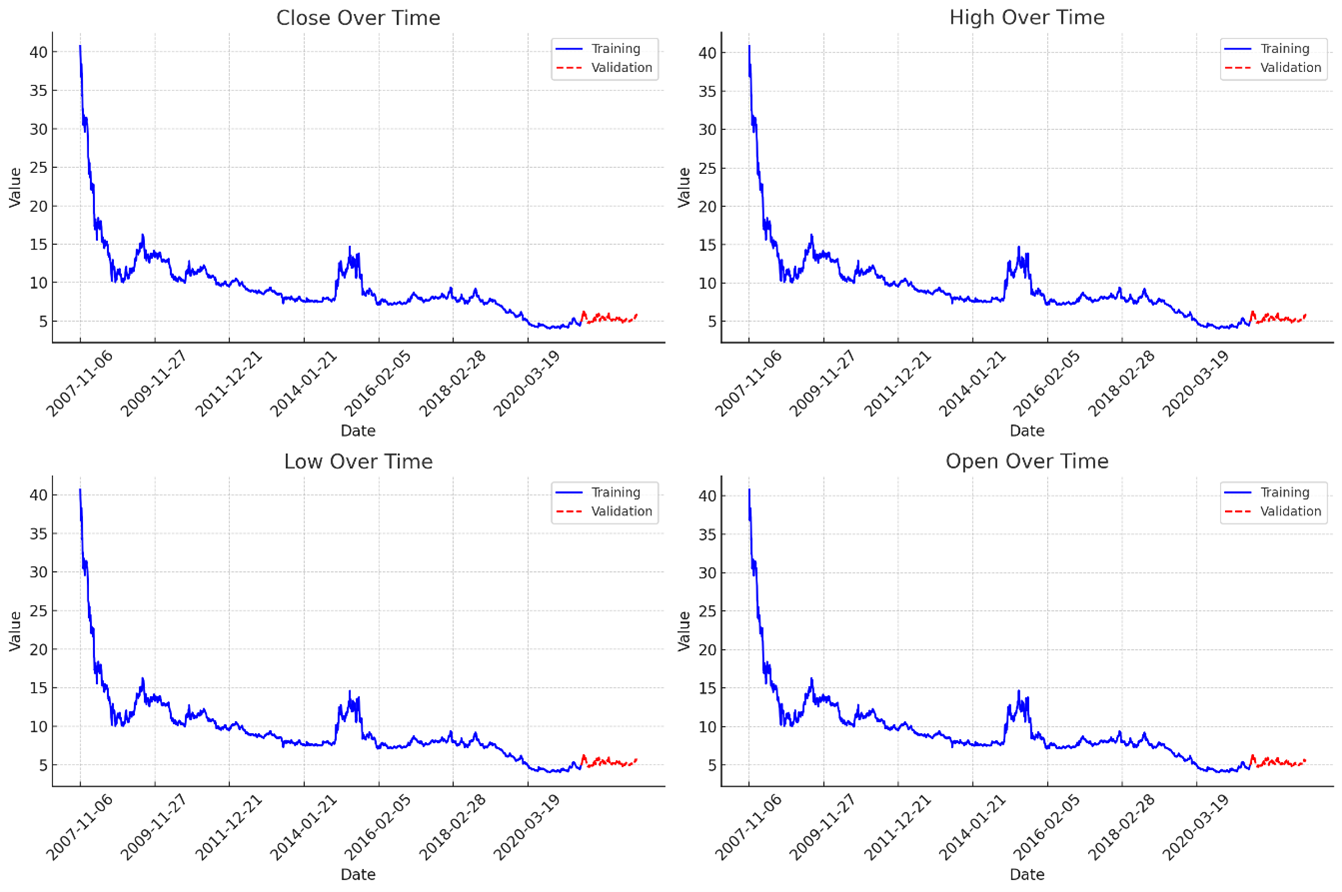
\includegraphics[width=1\textwidth]{pngs/dataset.png}
    \caption{ Data set}
    \label{dataset}
\end{figure}

Then we meticulously selected a total of 29 indicators. These are bifurcated into fundamental and technical types, encompassing 8 and 21 metrics respectively.Fundamental Indicators:
\begin{itemize}
    \item Opening price
    \item Closing price
    \item Peak price within the designated period
    \item Trough price within the same interval
    \item Trading volume in Stock (unit specification contingent on the context)
    \item Aggregate trading volume
    \item Weighted price 
    \item Discrepancy between the highest and lowest prices
\end{itemize}

In the realm of Technical Indicators, our choices were informed by the seminal works of references \cite{kara2011prediction}, \cite{guresen2011using}, and \cite{achelis2005technical}. A more detailed tabulation of these indicators will be provided in the subsequent Table \ref{tab_1}.



\begin{table}[h]
\caption{Features Used in this Model}\label{tab_1}%
\begin{tabular}{@{}ccc@{}}
\toprule
Feature name & Number of lags/window size  & Number of features \\
\midrule
Open, Close, High, Low     & 1   & 4    \\
Weighted Price     & 2   & 2    \\
Volume(Stock), Volume(Currency)     & 1   & 2    \\
High - Low   & 1   & 2    \\
Return    & from 1 to 5   & 5    \\
Correlation MA5 and MA30   & 1   & 1    \\
Sum3, Sum5    & 5,3   & 2    \\
Sum5 - Sum3    & 1   & 1   \\
RSI(6, 14)    & 6,14   & 2    \\
Rate of change    & 9,14   & 2   \\
Williams R    & 1   & 1    \\
CCI & 1 & 1   \\
DEMA & 1 & 1 \\
\botrule
\end{tabular}
\end{table}

The indicators encompass a diverse set of financial metrics, each designed to encapsulate various facets of stock price dynamics. This includes five distinct return rates with different lag intervals, a weighted moving average, correlation coefficients between weighted moving averages at various lags, cumulative prices over different timeframes, and other relevant metrics. To elucidate on select indicators:
The \textit{Average True Range (ATR)} is computed as:
\begin{equation}
ATR = MA(TR,N)
\end{equation}
where \(MA(TR,N)\) is the moving average of \(TR\) over \(N\) periods, effectively representing the average price over the last \(N\) intervals. The true range at the \(t^{th}\) period, \(TR_t\), is given by:
\begin{equation}
TR_{t} = \max(High_t - Low_t, High_t - Close_{t-1}, Close_{t-1} - Low_{t})
\end{equation}
Here, \(High\), \(Low\), and \(Close\) denote the highest, lowest, and closing prices for the period, respectively.
The \textit{Relative Strength Index (RSI)} is defined as:
\begin{equation}
RSI = 100 - \frac{100}{1 + \frac{MA(U,N)}{MA(D,N)}}
\end{equation}
When the price exhibits an upward or downward movement, the following conditions apply:
\begin{align}
U_t &= Close_t - Close_{t-1}, \quad D = 0 \\
D_t &= Close_t - Close_{t-1}, \quad U = 0
\end{align}
For the \textit{Price Return}, the formula is:
\begin{equation}
Return_{i_{t}} = Close_t - Close_{t-i}
\end{equation}
The \textit{Rate of Change (ROC)} is given by:
\begin{equation}
ROC_{i_{t}} = 100 \times \left( \frac{Close_{t}}{Close_{t-i}} - 1 \right)
\end{equation}
Additionally, the \textit{Stochastic Oscillator}, which gauges momentum in the Bitcoin price, is calculated as:


\begin{equation}
K = 100\frac{Close-Low}{High-Low}
\end{equation}
\begin{equation}
\text{Stochastic oscillator} = MA(K,N)
\end{equation}

Lastly, the \textit{CCI (Commodity Channel Index)}, reflecting average price deviation, measures the mean deviation degree given a fixed price interval. It is formulated as:
\begin{align}
CCI &= \frac{TP - MC}{MD \times 0.015} \\
TP &= \frac{1}{3} (High + Low + Close) \\
MC &= MA(Close, N) \\
MD &= MA(MC - Close, N)
\end{align}





\subsubsection{Data Manipulation}\label{subsubsec2}

Taking into account the inherent volatility of stock prices in their chronological series, a differencing method was employed. Fig \ref{adf} and Table \ref{tab_2} representations elucidate the dataset's autocorrelation. Parallelly, the Augmented Dickey-Fuller (ADF) unit root test was executed, validating the series' stability post differencing.
\begin{figure}[h]
    \centering
    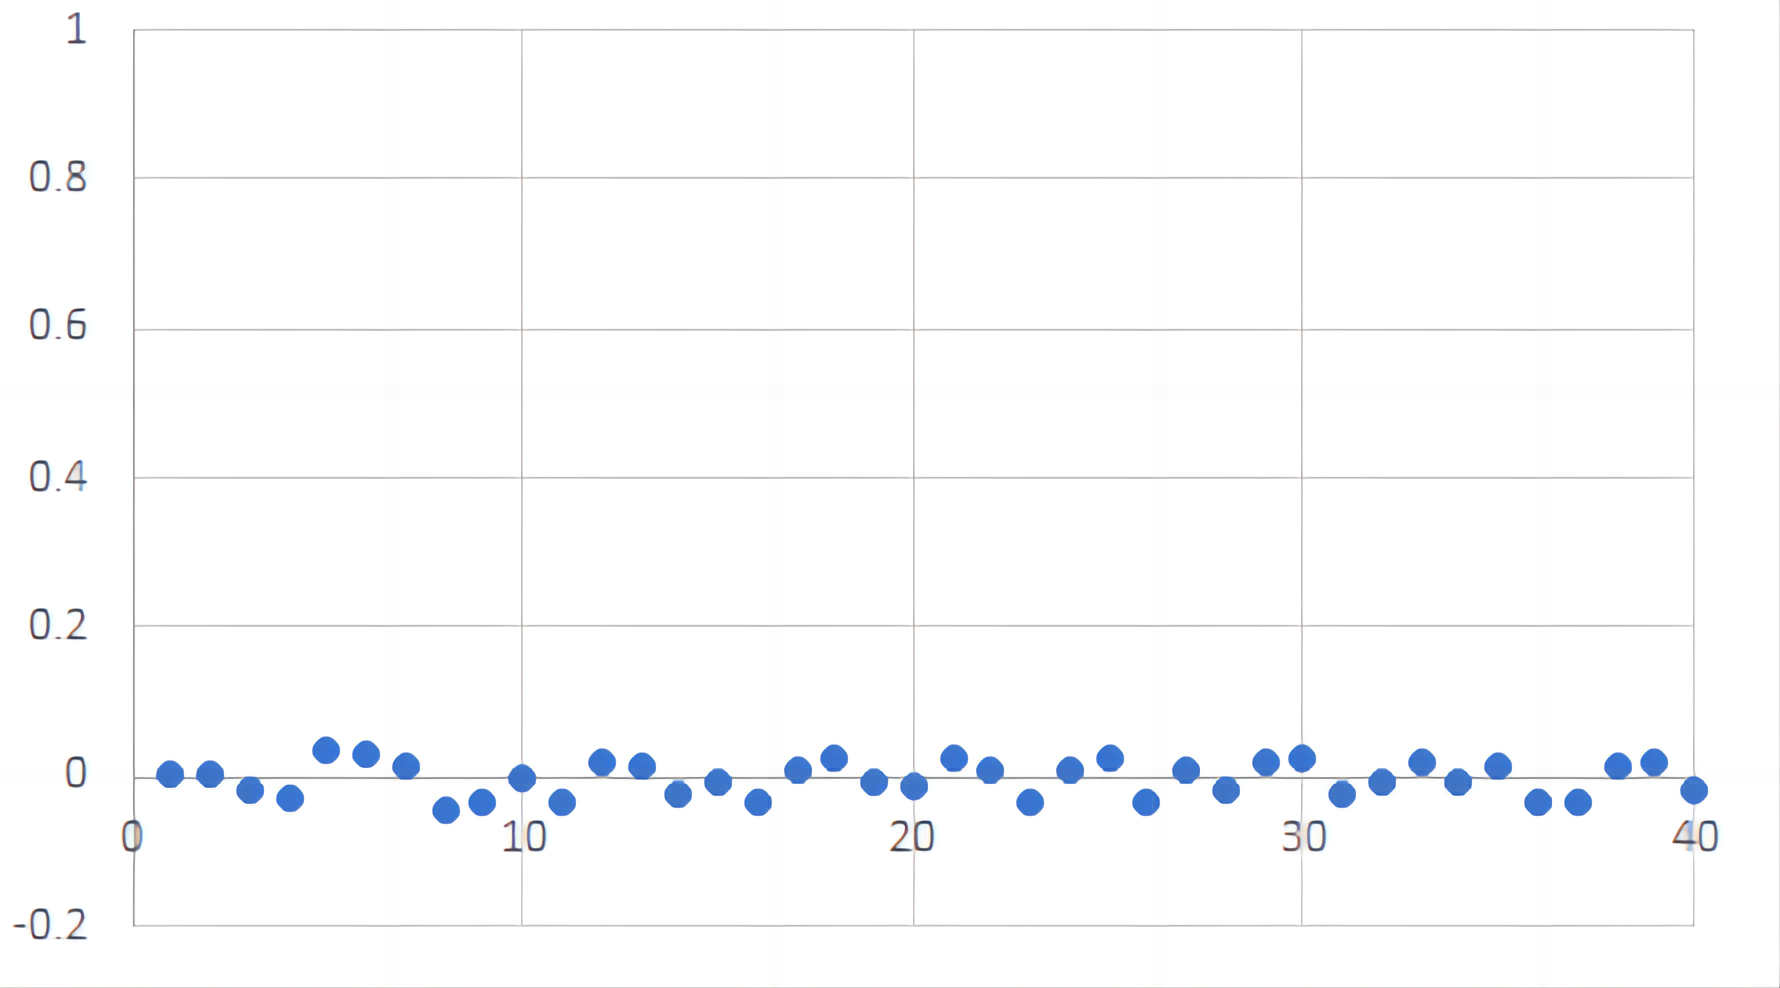
\includegraphics[width=0.5\textwidth]{pngs/adf.png}
    \caption{ Autocorrelation Graph}
    \label{adf}
\end{figure}

\begin{table}[h]
\centering
\caption{ADF Nnit Root Test}\label{tab_2}%
\begin{tabular}{@{}cc@{}}
\toprule
$Dickly-Fuller$ & -19.329573 \\
$p-value$ & 0.000000 \\
\bottomrule
\end{tabular}
\end{table}


A comprehensive descriptive statistical analysis was undertaken on all indicators, and both the raw and differenced data sets were subjected to the ADF examination. All differenced metrics successfully met the test criteria.

Given the heightened complexity inherent to stock prices, the natural logarithm of the terminal prices was extracted, followed by first-order differencing. The corresponding formula is presented as:

\begin{align}
new\: close_i=log(\cfrac{close_i}{close_{i-1}})
\end{align}
To enhance the efficiency of our neural network model, we standardized the 29 indicators. The calculation formula is:
\begin{align}
new\: value_i=\cfrac{value_i-E(value)}{\sqrt{D(value)}}
\end{align}
Where \( E(value) \) and \( D(value) \) represent the expected value and variance of the indicator, respectively.



\subsection{Model Architecture and Building}\label{subsec2}
In the process of constructing our stock price prediction model, a series of advanced methodologies were adopted to ensure both accuracy and robustness in forecasting. Initially, the VMD-MIC model was employed for feature decomposition and extraction, ensuring that clear and meaningful information is derived from intricate datasets. Subsequently, Fuzzy Entropy was applied for feature engineering, further refining the feature extraction process and enhancing the model's generalization capabilities. For the prediction phase, we utilized the stacked Informer framework, an amalgamation of various techniques, adept at capturing the dynamic fluctuations in stock prices with precision. To accurately assess the model's performance, a Dynamic Loss Function was designed, and in tandem with the Enhanced GC + Adam Optimizer, the model is fine-tuned to ensure optimal prediction outcomes in practical applications.

\subsubsection{VMD-MIC Model Framework}\label{subsec1}

Variance Mode Decomposition (VMD) is a sophisticated data decomposition technique, facilitates the transformation of time-domain financial sequences into the frequency domain\cite{dragomiretskiy2013variational}. This transformation yields a set of \( K \) intrinsic mode functions (IMFs). The foundational step in this procedure entails formulating the variational constraint equation:

\begin{equation}
\left\{\begin{array}{l}
\min \left\{\sum_{K=1}^K\left\|\partial_t\left[\left(\delta(t)+\frac{i}{\pi t}\right) * u_K(t)\right] e^{-i w_K t}\right\|_2^2\right\} \\
\text { s.t. } \sum_{K=1}^K u_K=x(t)
\end{array}\right.
\end{equation}

Here, \( x(t) \) denotes the financial data sequence. The terms \( w_K \) and \( u_K \) respectively represent the central frequency and band components of the \( k \)-th IMF. The impulse function is represented by \( \delta(t) \), while \( \partial t \) indicates the derivative with respect to time. The convolution operation (*) signifies the convolution computation in this context.

For a more tractable representation, the variational constraint equation is restructured using the Lagrange function \( \lambda(t) \) and the penalty factor \( \alpha \):

\begin{equation}
\begin{aligned}
L\left(\left\{u_K\right\},\left\{w_K\right\}, \lambda\right) &= \alpha \sum_{K=1}^K \left\| \partial_t \left[ \left( \delta(t) + \frac{i}{\pi t} \right) * u_K(t) \right] e^{-i w_K t} \right\|_2^2 \\
&+ \left\| x(t) - \sum_{K=1}^K u_K(t) \right\|_2^2 \\
&+ \left\langle \lambda(t), x(t) - \sum_{K=1}^K u_K(t) \right\rangle
\end{aligned}
\end{equation}
This reformulation alleviates the constraints, rendering the problem more manageable. The optimal solution is then determined using the Alternating Direction Method of Multipliers (ADMM), a renowned optimization technique. The iterative steps are as follows:

\begin{equation}
\begin{gathered}
\hat{u}_K^{n+1}(w)=\frac{\hat{x}(w)-\sum_{i \neq K} \hat{u}_j(w)+(\hat{\lambda}(w) / 2)}{1+2 \alpha\left(w-w_K\right)^2} \\
\end{gathered}
\end{equation}
\begin{equation}
\begin{gathered}
w_K^{n+1}=\frac{\int_0^{\infty} w\left|\hat{u}_K^{n+1}(w)\right|^2 d w}{\int_0^{\infty}\left|\hat{u}_K^{n+1}(w)\right|^2 d w}
\end{gathered}
\end{equation}
Following this sequence, the primary financial data sequence is decomposed into \( K \) distinct sub-series.

While VMD is underpinned by a robust mathematical framework and adept at disentangling complex signal components, it's constrained by the need for predetermined decomposition parameters. This requirement can compromise the fidelity of the decomposition. To address these limitations, this study proposes an amalgamation of VMD with the Mutual Information Coefficient (MIC)\cite{lin2022using}. This integration determines the optimal number of decompositions, \( K \), enhancing the decomposition's adaptability.

The degree of decomposition is judiciously determined via the MIC value between the original sequence, denoted as \( y \), and its reconstructed counterpart, \( y_0 \). A \( MICyy0 \) value closer to one indicates a higher fidelity in the VMD decomposition, translating to minimal information loss and an optimal decomposition result.


\subsubsection{Fuzzy Entropy approach}\label{subsec2}

Fuzzy Entropy (FE) serves as a prominent technique tailored for assessing the complexity inherent in temporal series, offering a profound insight into the intricacies of the data structure \cite{chen2009measuring}. A salient feature of FE is its adaptive nature, which allows for a seamless evolution in accordance with changes in its prescribed parameters. This adaptability confers upon FE a robust defense mechanism against noise-induced perturbations, ensuring its integrity even in the presence of external disturbances.

For a time series of length \( n \), the FE algorithm is seamlessly integrated within the framework governed by fuzzy membership functions. This methodological integration results in the subsequent formulation:
\begin{align}
D(x) = e^{-\ln(2)\left(\frac{x}{r}\right)^{2}}
\end{align}
Here, \( r \) represents the similarity tolerance, and \( x \) is equated to \( d^{m}_{ij} \), the distance between vectors that reconstruct the time series in an \( m \)-dimensional phase space. For \( i, j = 1, 2, \ldots, n - m + 1 \), taking an average over each \( i \) in \( D^{m}_{ij} \) produces the average similarity function:
\begin{equation}
\phi^m(r) = \frac{1}{N-m+1} \sum_{i=1}^{N-m+1}\left(\frac{1}{N-m} \sum_{j=1, j \neq i}^{N-m+1} D_{i j}^m\right)
\end{equation}
Subsequently, the FE can be expressed as:
\begin{equation}
FuzzyEn(m, r, n) = \ln\left(\frac{\Phi{}^{m}(r)}{\Phi{}^{m+1}(r)}\right)
\end{equation}

\subsubsection{stacked Informer structure}\label{subsec3}

In many practical applications, accurate prediction of long sequence time series (LSTF) is paramount, especially in the context of financial time series forecasting. Such predictions offer crucial early warnings for financial markets, ensuring their stability and safety. Commonly employed models, such as Recurrent Neural Networks (RNNs), Long Short-Term Memory (LSTM), and Transformers, have been applied in forecasting tasks\cite{vaswani2017attention}\cite{selvin2017stock}\cite{ye2019river}. However, due to architectural constraints, their performance in LSTF scenarios leaves room for improvement. Several studies \cite{zhou2021informer}\cite{pascanu2013difficulty} have indicated that the inherent design of these models struggles to capture long-range dependencies between inputs and outputs, limiting their effectiveness in LSTF tasks.

To address this challenge, Zhou et al. introduced a novel LSTF model based on the Transformer architecture, termed "Informer" \cite{zhou2021informer}. Compared to traditional approaches, the Informer boasts notable advantages:

\noindent (1) It incorporates the probSparse self-attention mechanism, significantly enhancing sequence alignment capabilities.

\noindent (2) Leveraging self-attention distillation techniques, the model effectively reduces the number of stacked layers, thereby improving its efficiency in processing long sequences.

\noindent (3) By employing a generative decoder, it is capable of predicting a substantial number of time series in a single forward pass, markedly accelerating inference speed.

The Informer framework is a sophisticated deep learning construct that primarily incorporates stacked self-attention layers. Intrinsically, this model adheres to the encoder-decoder paradigm, as depicted in Figure \ref{informer}.

\begin{figure}[h]
    \centering
    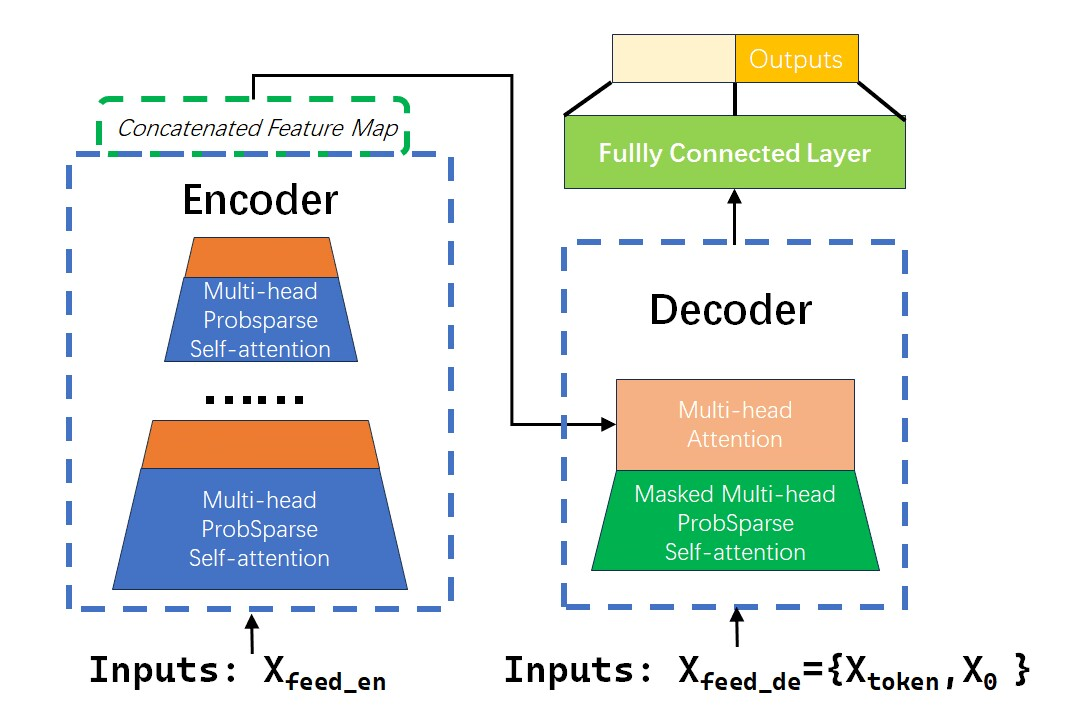
\includegraphics[width=0.6\textwidth]{pngs/informer.png}
    \caption{ Informer Model Structure}
    \label{informer}
\end{figure}
For a designated time \( t \), the model's input is characterized as:
\begin{align}
x^{t} = \lbrace x_{1}^{t}, \dots, x^{t}_{L_{x}} | x_{i}^{t} \in \mathbb{R}^{d_{x}} \rbrace
\end{align}
Simultaneously, the anticipated output of the model is defined as:
\begin{align}
y^{t} = \lbrace y_{1}^{t}, \dots, y^{t}_{L_{y}} | y_{i}^{t} \in \mathbb{R}^{d_{y}} \rbrace
\end{align}
The conventional self-attention mechanism operates via the \( (Query, Key, Value) \) triplet. This mechanism executes the scaled dot product of these inputs in the following manner:
\begin{align}
A(Q, K, V) = \text{Softmax}\left(\frac{QK^T}{\sqrt{d}}\right) V
\end{align}
Wherein \( Q, K, V \) are matrices of dimension \( \mathbb{R}^{L \times d} \).The probabilistic representation of the self-attention coefficient, for the \( i-th \) Query, is articulated as:
\begin{align}
A(q_i, K, V) = \mathbb{E}_{p(k_j | q_i)}\left[v_j\right]
\end{align}

While the inherent time complexity of the self-attention operation stands at \( O(L^2) \), empirical studies indicate that its resultant probability distribution assumes a long-tailed configuration. By strategically concentrating on select dot product pairings, computational demands can be optimized with minimal accuracy concessions. To actualize this, the Informer model introduces the ProbSparse self-attention mechanism. The sparsity evaluation for the \( i-th \) Query is formulated as:
\begin{align}
M(q_i, K) = \ln \sum_{j=1}^{L_K} e^{\frac{q_i k_j^T}{\sqrt{d}}} - \frac{1}{L_K} \sum_{j=1}^{L_K} \frac{q_i k_j^T}{\sqrt{d}}
\end{align}
The primary term signifies the log-sum-exp operation of the dot products between \( q_i \) and all Keys, while the latter term represents their average. Through the implementation of ProbSparse sampling, the self-attention operation's time complexity is efficiently reduced to \( O(L\log L) \).

In the encoder phase, the Informer employs Self-attention Distilling to accentuate the dataset's salient features. This methodology not only prioritizes predominant features but also fosters an improved self-attention feature mapping for ensuing layers. The transition process from layer \( j \) to \( j+1 \) is represented as:
\begin{align}
X_{j+1}^t = \text{MaxPool}\left(\text{ELU}\left(\text{Conv1d}\left(X_{j}^{t}\right)_{AB}\right)\right)
\end{align}
Here, the \( [·]_{AB} \) notation embodies operations such as multihead ProbSparse computations.

The decoder segment of the Informer adopts a traditional structure, incorporating a pair of consistent multi-head self-attention layers. The input vector for this phase is expressed as:
\begin{equation}
X_{\text{feed\_de}}^t = \text{Concat}\left(X_{\text{token}}^t, X_0^t\right) \in \mathbb{R}^{\left(L_{\text{token}} + L_y\right) \times d_{\text{model}}}
\end{equation}
Utilizing Masked Multihead Attention within this layer, the Informer model sidesteps potential autoregressive scenarios. The model's conclusive predictions are conveyed through a densely connected layer, with the mean square error (MSE) serving as the loss function.


In the realm of long-term time series forecasting, numerous established models exist. Yet, achieving high-precision predictions remains a formidable challenge. To better capture long-range dependencies in time series and enhance forecast accuracy, we introduce an innovative framework: the Stacked Informer Structure.

As illustrated in the Fig \ref{sinformer}, we depict the stacked architecture, an enhanced and tiered rendition of the multilayer Informer network. Within the context of the Stacked Informer Structure, consider the original long time series data input, denoted as \( L \). This sequence \( L \) undergoes an initial halving (to \( L/2 \)), followed by a subsequent division into quarters (to \( L/4 \)). The input \( L \) is then processed through a series of three attention blocks and two convolution layers. Similarly, the \( L/2 \) sequence traverses two attention blocks and one convolution layer, while the \( L/4 \) sequence passes through a singular attention block. Ultimately, features extracted from all three \( L/8 \) dimensional sequences are amalgamated to forge an integrated feature map, which is subsequently channeled to the decoding module.
\begin{figure}[h]
    \centering
    \includegraphics[width=1\textwidth]{pngs/sinformer.png}
    \caption{ Proposed Stacked Structure of network}
    \label{sinformer}
\end{figure}
The primary objectives underscoring this stacked architectural configuration are twofold: first, to effectively distill intrinsic temporal features present in the input long time-series sequence; and second, to bolster the robustness and resilience of the forecasted fault sequence output. To achieve these dual aims, the Stacked Informer Structure incorporates a multi-scale input representation, where distinct temporal scales are processed through varied pathways. This ensures the model's capability to capture diverse features across different temporal scales, thereby enriching the information provision in long-term forecasting tasks. Moreover, by integrating features from varied scales into a cohesive feature map, the model effectively considers interactions and dependencies across scales. For each scale, attention blocks are employed to capture long-range dependencies in the input sequence. The design of these attention blocks is rooted in the Transformer architecture, renowned for its efficacy in capturing long-range dependencies. Additionally, convolution layers are deployed to distill local features, which are subsequently amalgamated with outputs from the attention blocks. In essence, through the adoption of the Stacked Informer Structure, we can adeptly capture intricate patterns and dependencies within long time series, culminating in more precise predictions.

\subsubsection{Dynamic Loss Function}\label{subsec4}

The adaptive loss function, a novel approach to loss function formulation, was pioneered in the work of Barron \cite{barron2019general}. This approach integrates a continuous parameter signifying robustness into the traditional loss function. Throughout the optimization phase of model training, this dynamic loss function refines the robustness parameters in tandem with the loss minimization procedure, enhancing prediction precision. The generalized loss function is mathematically described as:
\begin{equation}
f(z, \beta, c) = \frac{|\beta-2|}{\beta}\left(\left(\frac{(z / c)^2}{|\beta-2|}+1\right)^{\beta / 2}-1\right)
\end{equation}

In this formulation, the variable \(z\) quantifies the residual between observed and predicted values. The positive scalar \(c > 0\) adjusts the curvature of the quadratic component at \(x = 0\), while \(\beta\) serves as the adaptable parameter steering robustness.

A detailed examination of the equation reveals that the behavior of the adaptive loss function is intricately tied to variations in \(\beta\). Different settings of \(\beta\) manifest in the loss function as:
\begin{equation}
L(z, \beta, c) = 
\begin{cases}
\frac{1}{2}(z / c)^2 & \text{if } \beta=2 \\
\log \left(\frac{1}{2}(z / c)^2+1\right) & \text{if } \beta=0 \\
\sqrt{(z / c)^2+1}-1 & \text{if } \beta=1 \\
1-\exp \left(-\frac{1}{2}(z / c)^2\right) & \text{if } \beta=-\infty \\
\frac{|\beta-2|}{\beta}\left(\left(\frac{(z / c)^2}{|\beta-2|}+1\right)^{\beta / 2}-1\right) & \text{otherwise}
\end{cases}
\end{equation}

It is noteworthy that this adaptive loss function is versatile, enveloping a spectrum of loss functions such as Mean Squared Error (MSE), Cauchy, Charbonnier, and Welsch. This versatility is attributed to the modulation of the \(\beta\) parameter, which grants the flexibility to customize the loss function per specific modeling needs.

Incorporating such a loss function into long-term time series forecasting models can be advantageous. Its adaptability allows for nuanced error handling, potentially leading to improved model robustness and sensitivity to various data patterns, especially in scenarios with non-Gaussian noise or outliers.


\subsubsection{ GC-Enhanced Adam Optimizer}\label{subsec5}

Optimization strategies are of paramount importance in the effective and efficient training of Deep Neural Networks (DNNs). While traditional optimizers such as Stochastic Gradient Descent (SGD) and Adam have been widely adopted in DNNs, this work incorporates the novel Gradient Centralization (GC) technique into the Adam optimizer, aiming to further enhance its efficacy.

The GC technique was pioneered by Yong et al. in 2020 \cite{yong2020gradient}. Unlike other methods that modify the learning rates or adaptively adjust weights, GC directly acts upon the gradients by centralizing them, effectively making their mean values zero. One can draw parallels between GC and projected gradient descent, though the former operates within the constraints of a specific loss function. This centralization is believed to foster a more stable and efficient training process.

Given a weight vector \( \mathbf{w} \), with corresponding gradients denoted as \( \nabla w_i L \) (where \( i \) spans from 1 to \( N \)), the GC operator, \( \phi_{\text{GC}} \), is formally defined as:

\begin{equation}
\phi_{\text{GC}}\left(\nabla_{w_i} L\right) = \nabla_{w_i} L - \mu \nabla w_i L
\end{equation}
Here, 
\begin{equation}
\mu \nabla_{w_i} L = \frac{1}{M} \sum_{j=1}^M W_{i, j} L
\end{equation}
Where \( M \) denotes the dimensionality, and \( L \) is the objective function. The essence of this formulation is the subtraction of the computed mean of column vectors in the weight matrix from each individual column vector, achieving gradient centralization.

For a more matrix-oriented representation, one can express the aforementioned operation as:
\begin{equation}
\phi_{\text{GC}}\left(\nabla_W L\right) = P \nabla_W L, \quad P = I - e e^T
\end{equation}
In this formulation, \( \mathbf{W} \) is the weight matrix, \( \mathbf{P} \) is the projection matrix that lies within the hyperplane defined by a normal vector in the weight space, and \( \mathbf{P} \nabla \mathbf{W} L \) is the gradient projected onto said hyperplane. Once the centralized gradient \( \phi_{\text{GC}}(\nabla \mathbf{W} L) \) is obtained, it can be seamlessly used for weight matrix updates.

One potential enhancement to consider when employing GC with Adam or other adaptive optimizers is the careful tuning of hyperparameters. While GC aims to stabilize the training process, the adaptive nature of optimizers like Adam means that they adjust learning rates based on past gradient moments. Combining these two methodologies might necessitate a recalibration of hyperparameters to achieve optimal results.

\subsubsection{ The Overall Framework of the Prediction Model}\label{subsec5}

Given the intrinsic volatility of financial sequence data, the present research proposes a holistic predictive framework that synergistically integrates five pivotal components: VMD-MIC, Fuzzy Entropy (FE), a stacked Informer structure, a dynamic loss function, and a GC-enhanced Adam optimizer as shown in the Fig\ref{all}.

\begin{figure}[h]
    \centering
    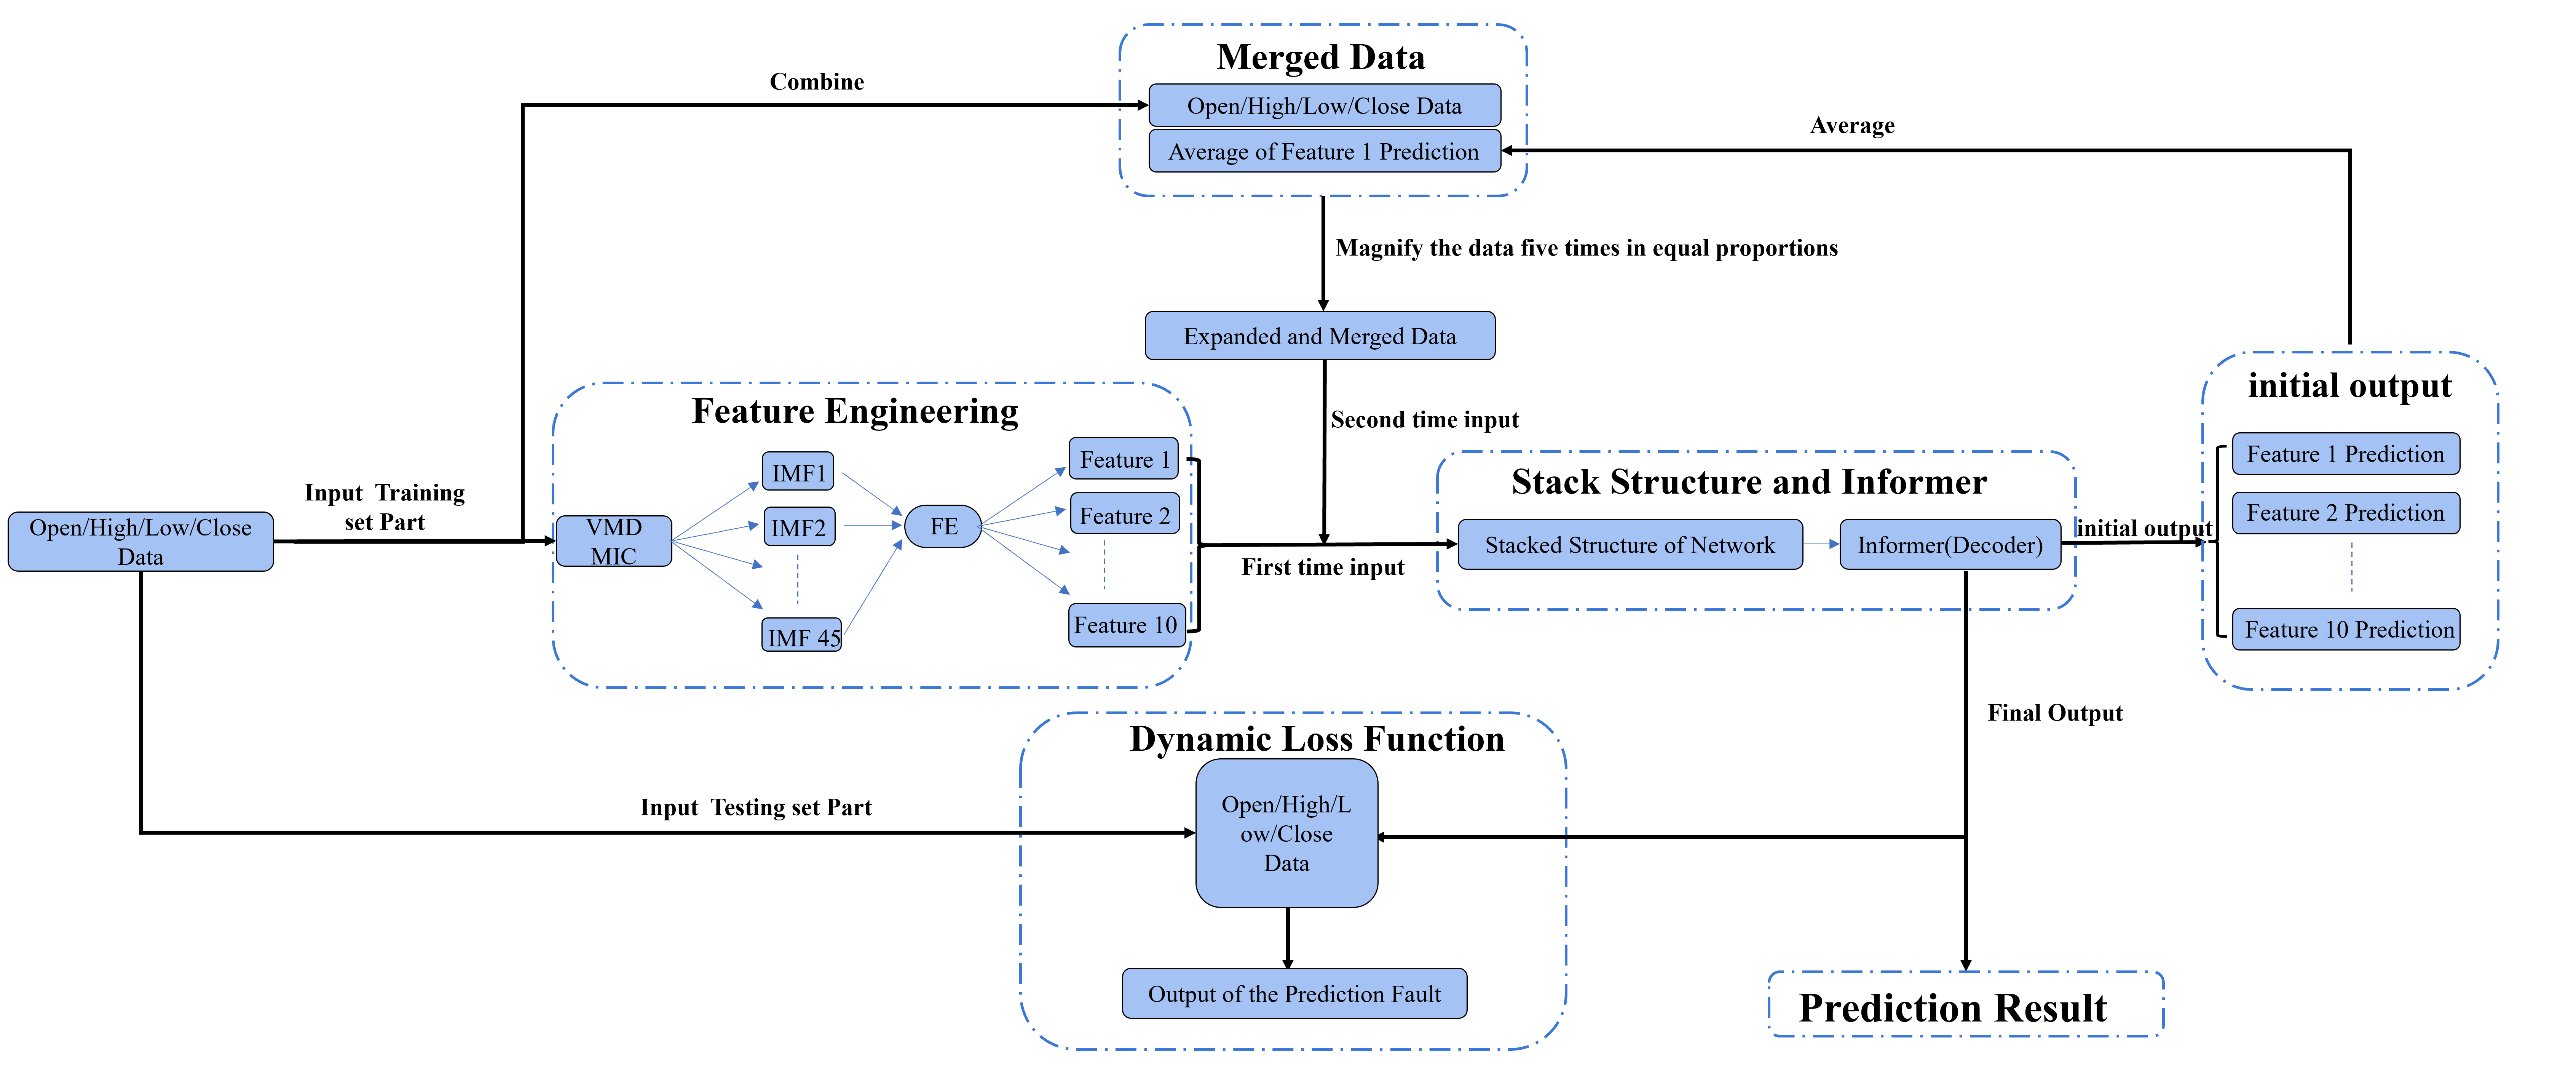
\includegraphics[width=0.95\textwidth]{pngs/all.png}
    \caption{ Overall Framework of the Prediction Model}
    \label{all}
\end{figure}

\begin{enumerate}
\item \textbf{Data Decomposition with VMD-MIC}: 
At the inception of our data preprocessing, the original financial data, comprising 29 unique features, is subjected to Variance Mode Decomposition (VMD), resulting in a series of K Intrinsic Mode Functions (IMFs). The VMD-MIC method stands out for its ability to transform time-domain financial sequences into the frequency domain, offering a nuanced perspective on the inherent patterns of the data.
    
\item \textbf{Complexity Measurement via Fuzzy Entropy}:
Post decomposition, the Fuzzy Entropy (FE) technique is employed to gauge the complexity of each individual IMF. This quantification not only provides insights into the intricacies of the data structure but also facilitates the amalgamation of IMFs that bear similar characteristics, leading to the generation of reconstructed components.
    
\item \textbf{Feature Selection and Input Preparation}:
Leveraging the MIC algorithm, salient features are meticulously selected from the processed data. These curated features serve as the foundation upon which the subsequent predictive modeling is constructed.
    
\item \textbf{Prediction with Stacked Informer}:
The heart of our framework is the stacked Informer structure. Built upon advanced architectures like Long Short-Term Memory (LSTM) and Transformers, this model is specifically tailored for long sequence time series forecasting, ensuring impeccable accuracy.
    
\item \textbf{Optimization via GC-Enhanced Adam}:

As we delve into the training phase, the GC-enhanced Adam optimizer comes into play. By incorporating the novel Gradient Centralization technique, this optimizer promises rapid convergence and robust model performance, setting it apart from traditional optimization methods.
\end{enumerate}

To synthesize the outputs from the various components, a weighted ensemble approach is adopted. Specifically, the outputs are combined using a weighted average, where the weights are determined based on each model's performance on a validation set. This ensures that models with superior performance have a more significant influence on the final prediction, providing a refined forecasting curve that captures the intricate nuances of financial time series.

\subsection{ Evaluation indicators}\label{subsec3}
The mean absolute error (MAE), mean square error (MSE), root mean square error (RMSE), and coefficient ofdetermination (R2) are used as indicators for the prediction performance of
our VMGCformer and all the other models. The formulas of each indicators are as follow:
\begin{equation}
MAE = \frac{1}{N} \sum_{t=1}^N \left| q_{\text{true}}(t) - q_{\text{pred}}(t) \right|
\end{equation}
\begin{equation}
MSE={\frac{1}{N} \sum_{t=1}^N\left(q_{\text {true }}(t)-q_{\text {pred }}(t)\right)^2} 
\end{equation}
\begin{equation}
RMSE=\sqrt{\frac{1}{N} \sum_{t=1}^N\left(q_{\text {true }}(t)-q_{\text {pred }}(t)\right)^2} 
\end{equation}
\begin{equation}
R^2=1-\frac{\sum_{t=1}^N\left(q_{\text {true }}(t)-q_{\text {pred }}(t)\right)^2}{\sum_{t=1}^N\left(q_{\text {true }}(t)-\bar{q}\right)^2}
\end{equation}



\section{Feature extraction and experimental results}\label{sec4}
\subsection{Experimental environment and configuration}\label{subsubsec1}
Regarding the experimental configuration, our comprehensive investigations are carried out utilizing a computer system endowed with dual NVIDIA GeForce RTX 4090 GPUs, accompanied by an Intel Xeon E5-2650 v3 @2.3GHz CPU and a robust 128GB RAM. The operational environment is governed by the Ubuntu22 operating system, while the deep learning framework employed throughout our endeavors remains PyTorch.

\subsection{Feature decomposition and feature engineering}\label{subsubsec1}
\subsubsection{Determination of K Value and decomposition of features}\label{subsubsec1}
The \textit{VMD-MIC} method enhances the conventional \textit{VMD} approach by utilizing the computation of the \textit{MICyy0} metric. When the original stock dataset is input into the \textit{VMD-MIC} framework, it is decomposed into \( K \) intrinsic mode functions (IMFs). Figure \ref{MICYY} illustrates the relationship between various \( K \) values and their corresponding \textit{MICyy0} results. 

\begin{figure}[h]
    \centering
    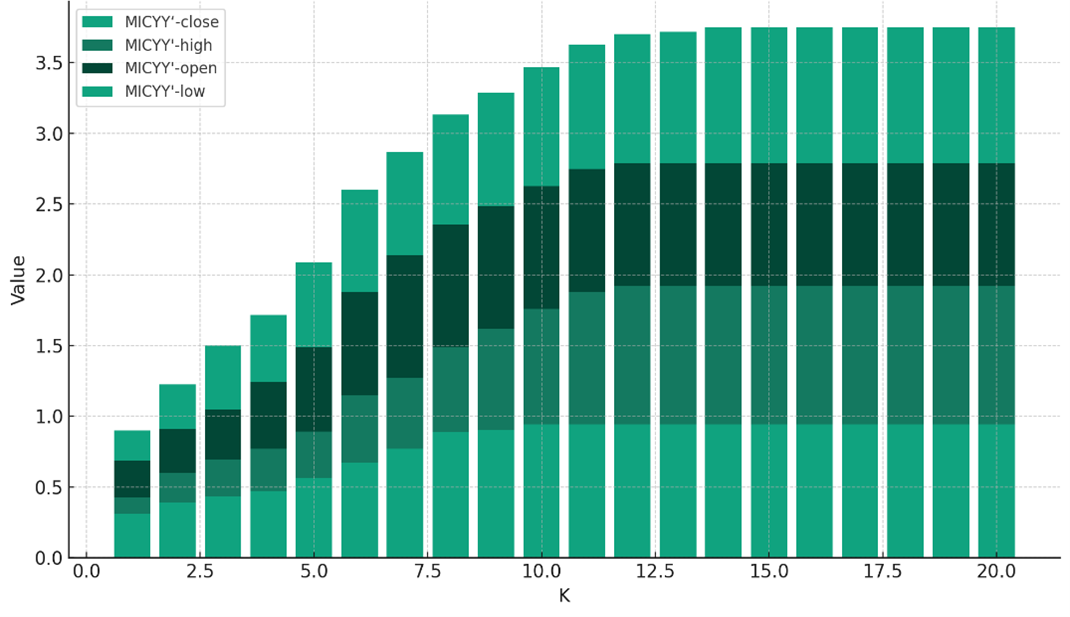
\includegraphics[width=0.75\textwidth]{pngs/MICYY.png}
    \caption{ Relationship Between Different $K$s and Their Corresponding \textit{MICyy0}}
    \label{MICYY}
\end{figure}


Notably, the \textit{MICyy0} metric remains relatively stable for \( K = 8, 10, 12 \) and \( 15 \). Based on this observation, we make the following selection of K values as shown in the Table\ref{tab_3}:

\begin{table}[h]
\caption{Selection of K Values}\label{tab_3}%
\begin{tabular}{@{}ccc@{}}
\toprule
indicator & the selection of K for corresponding indicator  \\
\midrule
Open      & 15    \\
Close    & 10    \\
High        & 12    \\
Low      & 8    \\
\botrule
\end{tabular}
\end{table}


Based on this premise, we have delineated the IMF values for the four features: close, high, low, and open prices, post-decomposition at varying \( k \) values as depicted in Fig\ref{IMF}. Correspondingly, we also present their associated Power Spectral Density (PSD) values in Fig\ref{PSD}. It is discerned that with the incremental growth of \( k \) values, their respective trends largely converge. By conducting an in-depth evaluation of the dominant frequencies in these IMF curves, we can discern the efficiency of the \textit{VMD-MIC} technique in ensuring precise IMF separation.

\begin{figure}[h]
    \centering
    \includegraphics[width=1\textwidth]{pngs/IMF.png}
    \caption{ The Decomposition Results For Each Feature: IMFs Values for Each k.}
    \label{IMF}
\end{figure}
\begin{figure}[h]
    \centering
    \includegraphics[width=1\textwidth]{pngs/PSD.png}
    \caption{ The Dcomposition Results For Each Feature: Power Spectral Density (PSD) for Each Corresponding IMFs.}
    \label{PSD}
\end{figure}


\subsubsection{Dimensionality reduction operation of features}\label{subsubsec2}

The original stock dataset was decomposed into intrinsic mode functions (IMFs) with allocations of 10 for close, 12 for high, 8 for low, and 15 for open values. Direct integration of these sub-sequences into the predictive model could exacerbate computational overhead. To address this, we employed Feature Extraction (FE) to quantitatively assess the intricacy of the IMFs, subsequently reconstituting them based on their complexity profiles. Through rigorous research, parameters m = 3 and r = 0.3std were delineated as optimal, striking a balance between model accuracy and computational efficiency. The corresponding visualization in Fig \ref{FE} elucidates the FE values for each IMF.
\begin{figure}[h]
    \centering
    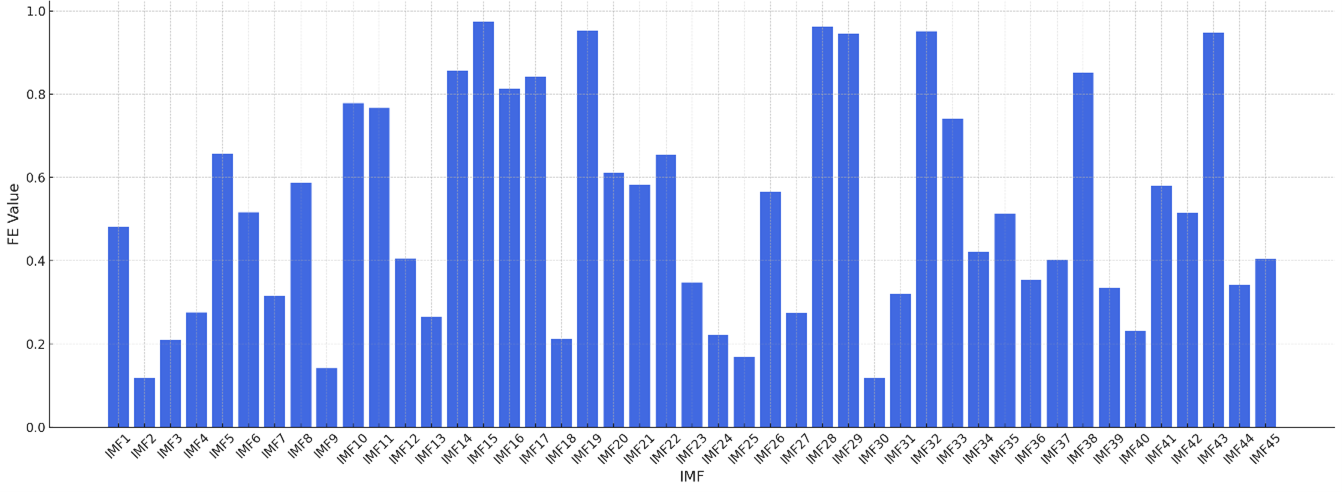
\includegraphics[width=0.9\textwidth]{pngs/FE.png}
    \caption{ FE Values for 45 IMFs}
    \label{FE}
\end{figure}




Upon categorization of IMFs by FE value intervals (e.g., 0.0-0.1, 0.1-0.2, etc.), we crafted new composite elements founded on these FE metrics as shown in the Table \ref{tab_4}.

\begin{table}[h]
\caption{New Composite Elements Founded FE Metrics}\label{tab_4}%
\begin{tabular}{@{}ccc@{}}
\toprule
New feature grouping & FE Value range & 
Selection of IMFn (value of n)  \\
\midrule
New feature1     & [0.0,0.1]   & none \\
New feature2     & (0.1,0.2]   & 2,9,25,30 \\
New feature3     & (0.2,0.3]   & 3,4,13,18,24,27,40 \\
New feature4     & (0.3,0.4]   & 7,23,31,36,37,39,44,45 \\
New feature5     & (0.4,0.5]   & 1,12,34 \\
New feature6     & (0.5,0.6]   & 6,8,21,26,35,41,42 \\
New feature7     & (0.6,0.7]   & 5,20,22 \\
New feature8     & (0.7,0.8]   & 10,11,33 \\
New feature9     & (0.8,0.9]   & 14,16,17,38 \\
New feature10    & (0.9,1.0]   & 15,19,28,29,32,43 \\

\botrule
\end{tabular}
\footnotetext{Note2: $\text{new feature}N  = \cfrac{\displaystyle\sum_{\text{selected } N} \text{IMF} N}{V}$,$V$ is the total number of selected IMFs.}
\end{table}



\subsubsection{Feature extraction and selection based on correlation}\label{subsubsec3}

In our endeavor to efficiently extract the residual 25 indicator features, we discerned that the computational efficacy and generalizability of the model could be enhanced by excluding certain irrelevant or redundant attributes from the primary dataset. Consequently, we adopted the Maximal Information Coefficient (MIC) methodology to scrutinize the interrelations between the remaining 25 stock features and each component, extracting quintessential characteristics of each element through their MIC values. The confusion matrix for MIC is depicted in the subsequent Heatmap of Features (Fig \ref{Heat Map}).
\begin{figure}[h]
    \centering
    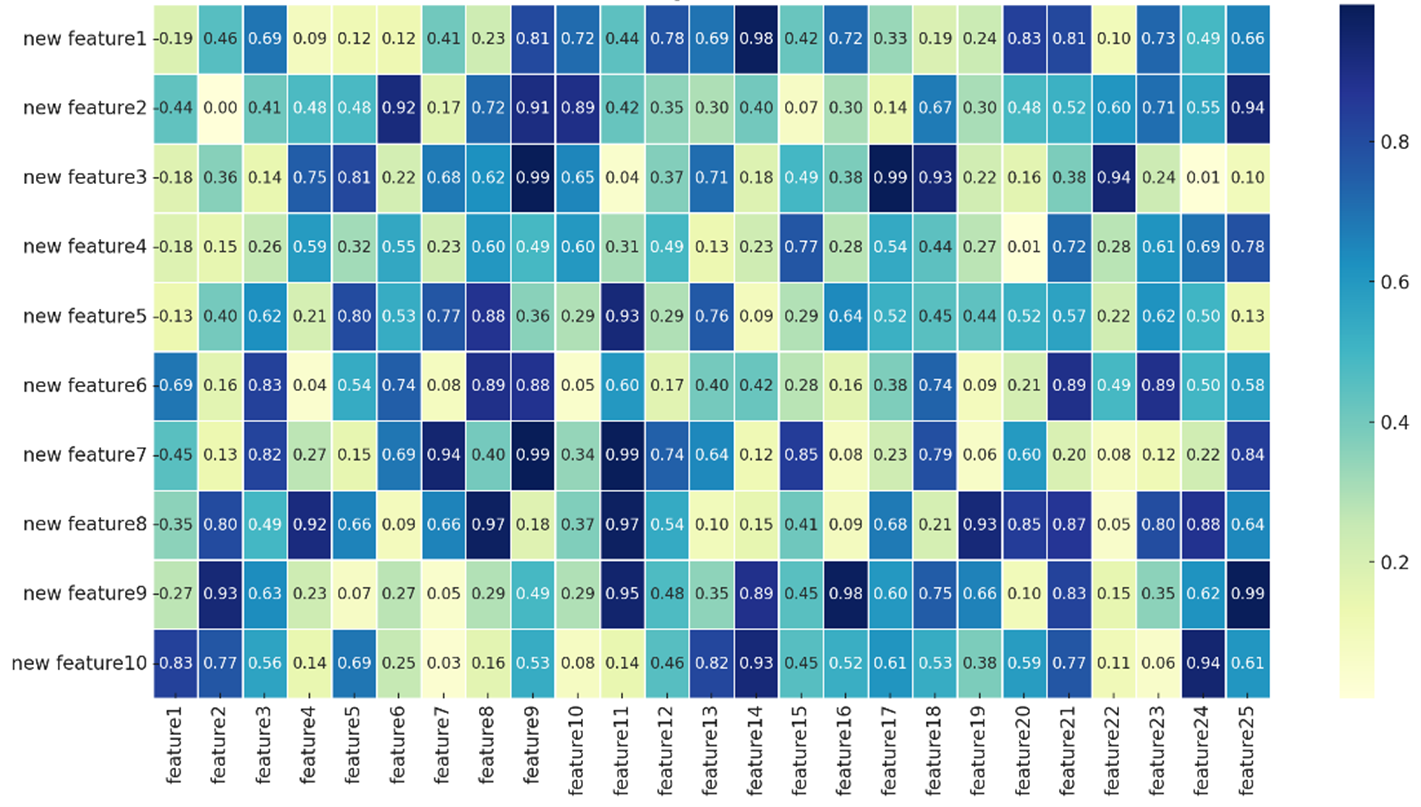
\includegraphics[width=1\textwidth]{pngs/Heat Map.png}
    \caption{ Heatmap For Features}
    \label{Heat Map}
\end{figure}

From the ensuing visualization, it's palpable that each element manifests distinct influential characteristics, encapsulating both holistic correlations and nuanced local attributes. In pursuit of curating features that bear the utmost correlation with the input variables, we instituted an MIC threshold of 0.8 for each component. The outcomes of this selective input feature determination are delineated in the Table \ref{tab_5} below.

\begin{table}[h]
\caption{Selection of Reconstructed Feature Values Based On Heatmap}\label{tab_5}%
\begin{tabular}{@{}ccc@{}}
\toprule
New feature grouping & 
Included New Feature M (M value) & 
Included Feature N (N value)  \\
\midrule
New feature1 reconstruct  & 1  & 2,3,7,9,10,11,12,13,14,15,16,20,21,23,24,25 \\
New feature2 reconstruct  & 2  & 3,4,5,6,8,9,10,11,14,18,20,31,22,23,24,25 \\
New feature3 reconstruct  & 3  & 4,5,7,8,9,10,13,15,17,18,22 \\
New feature4 reconstruct  & 4  & 4,6,8,9,10,12,15,17,18,21,23,24,25 \\
New feature5 reconstruct  & 5  & 2,3,5,6,7,8,11,13,16,17,18,19,20,21,23,24,25 \\
New feature6 reconstruct  & 6  & 1,3,5,6,8,9,11,13,14,18,21,22,23,24,25 \\
New feature7 reconstruct  & 7  & 3,6,7,8,9,11,12,13,15,18,20,25 \\
New feature8 reconstruct  & 8  & 2,3,4,5,7,8,11,12,15,17,19,20,21,23,24,25 \\
New feature9 reconstruct  & 9  & 2,3,9,11,12,14,15,16,17,18,19,21,24,25 \\
New feature10 reconstruct & 10 & 1,2,3,5,9,12,13,14,15,16,17,1820,21,24,25 \\
\botrule
\end{tabular}
\footnotetext{Note1: The features corresponding to all areas greater than 0.4 in the heatmap are selected into the corresponding group.}
\footnotetext{Note2: $\text{new feature}N \text{reconstruct} = \frac{\text{New Feature} M}{V} +\cfrac{\displaystyle\sum_{\text{selected } N} \text{Feature} N}{V}$,$V$ is the total number of selected parameters.}
\end{table}




\subsection{Model parameter configuration}\label{subsubsec1}
In this section, we delineate the rationale behind the selection of our model's parameters. After rigorous experimentation and meticulous debugging, we have judiciously chosen a set of parameters that optimally enhances the predictive capabilities of our model. The salient parameters integral to our model's architecture are delineated in Table \ref{tab_parameters}.

\begin{table}[h]
\caption{Model Parameters Configuration}\label{tab_parameters}%
\centering
\begin{tabular}{@{}cc@{}}
\toprule
\textbf{Parameter} & \textbf{Value} \\
\midrule
Input sequence length & 200 \\
Prediction sequence length & 64-128 \\
Num of encoder layers & 8 \\
Num of decoder layers & 10 \\
Input size of encoder & 5-1 \\
Input size of decoder & 5-1 \\
Num of heads & 8 \\
Dimension of model & 512 \\
Probsparse attention factor & 3.8 \\
Early stopping patience & 10 \\
Dropout & 0.2 \\
Epochs & 150 \\
\bottomrule
\end{tabular}
\end{table}


\subsection{Experiments and results}\label{subsubsec1}
In the experimental segment of this investigation, we integrated ten previously extracted features into our model, procuring predictions for these ten features. Subsequently, we computed their average and amalgamated this mean value with one of the four financial metrics: "open", "high", "low", or "close". The consolidated data was then linearly amplified by a factor of five and re-input into our model to forecast the aforementioned financial indicators. This procedure is graphically delineated in the architecture presented in Fig. \ref{arche}. We then input the results into Laoo Function to calculate the error.

\begin{figure}[h]
    \centering
    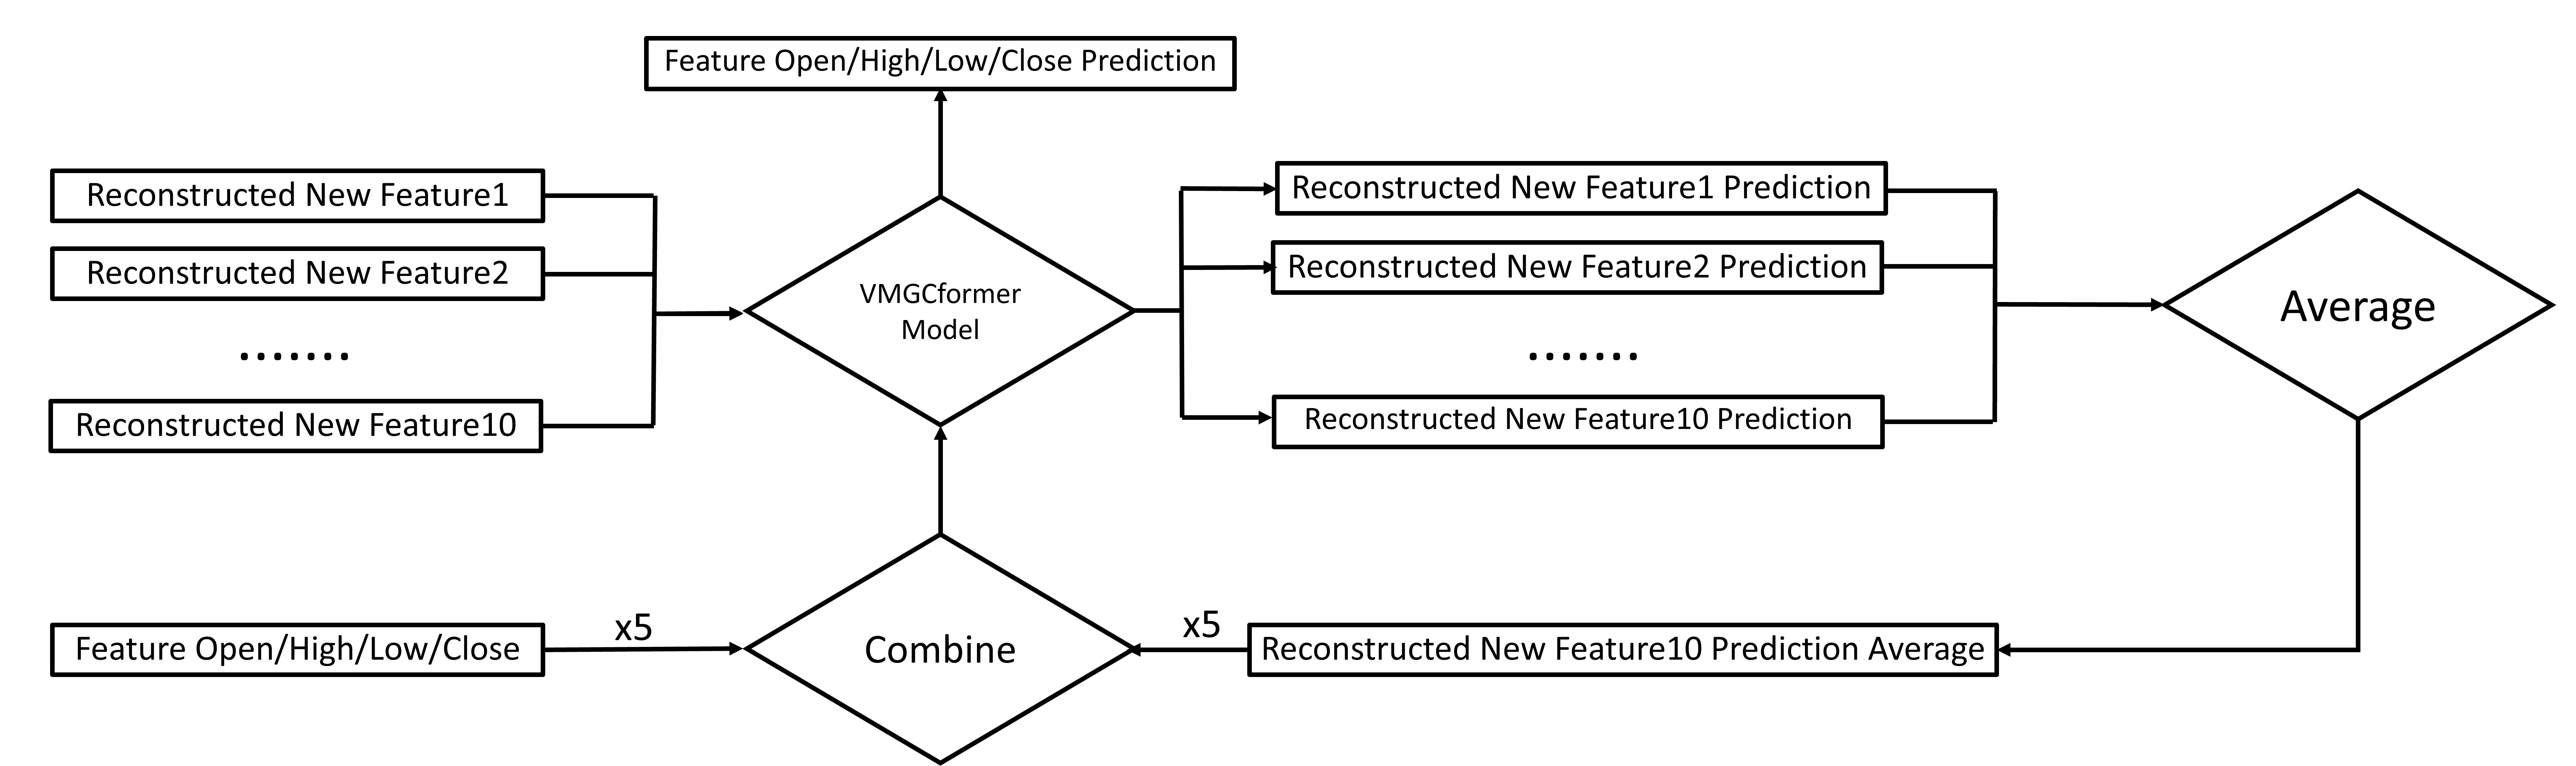
\includegraphics[width=1\textwidth]{pngs/arche.png}
    \caption{Structure of The Experiment}
    \label{arche}
\end{figure}

To evaluate the superiority of each module within the model as well as its overall performance, we conducted ablation studies and comparative experiments. Furthermore, to assess the generalizability and robustness of our model, we performed stability tests on several additional stocks. Due to space constraints, we presented only the prediction results for the "open" indicator in the ablation studies, selected the "high" indicator for the comparative experiments, and showcased the "low" indicator in the stability tests. The indicators chosen typically demonstrated median predictive performance in their respective experiments, a selection approach designed to minimize potential biases arising from random factors.

\subsubsection{Ablation Experiment}\label{subsubsec1}

The objective of the ablation study is to verify whether the intricate hybrid model enhances prediction accuracy in comparison to simpler composite models and standalone models. The benchmark models we selected include Adam+GC+enhanced informer (In the ablation study, for ease of description and comparison, we refer to VMGCformer as Adam+GC+enhanced informer) , Adam+GC+informer, Adam+enhanced informer, and Adam+informer. The corresponding parameters were obtained via grid search methods, where the robustness parameter \( \beta \) is adaptively adjusted by the Adam optimizer. Specific parameters are detailed in the Table \ref{tab_parameters}. Both the encoder and the decoder have input sizes equivalent to the number of input variables of the model.

As depicted in Fig. \ref{loss}, the training outcomes for the four models are presented. It is evident that the forecasting approach utilizing Adam+GC+informer consistently achieves stability more rapidly and attains the lowest error rates on both the training and test sets, aligning with our initial expectations.

\begin{figure}[h]
    \centering
    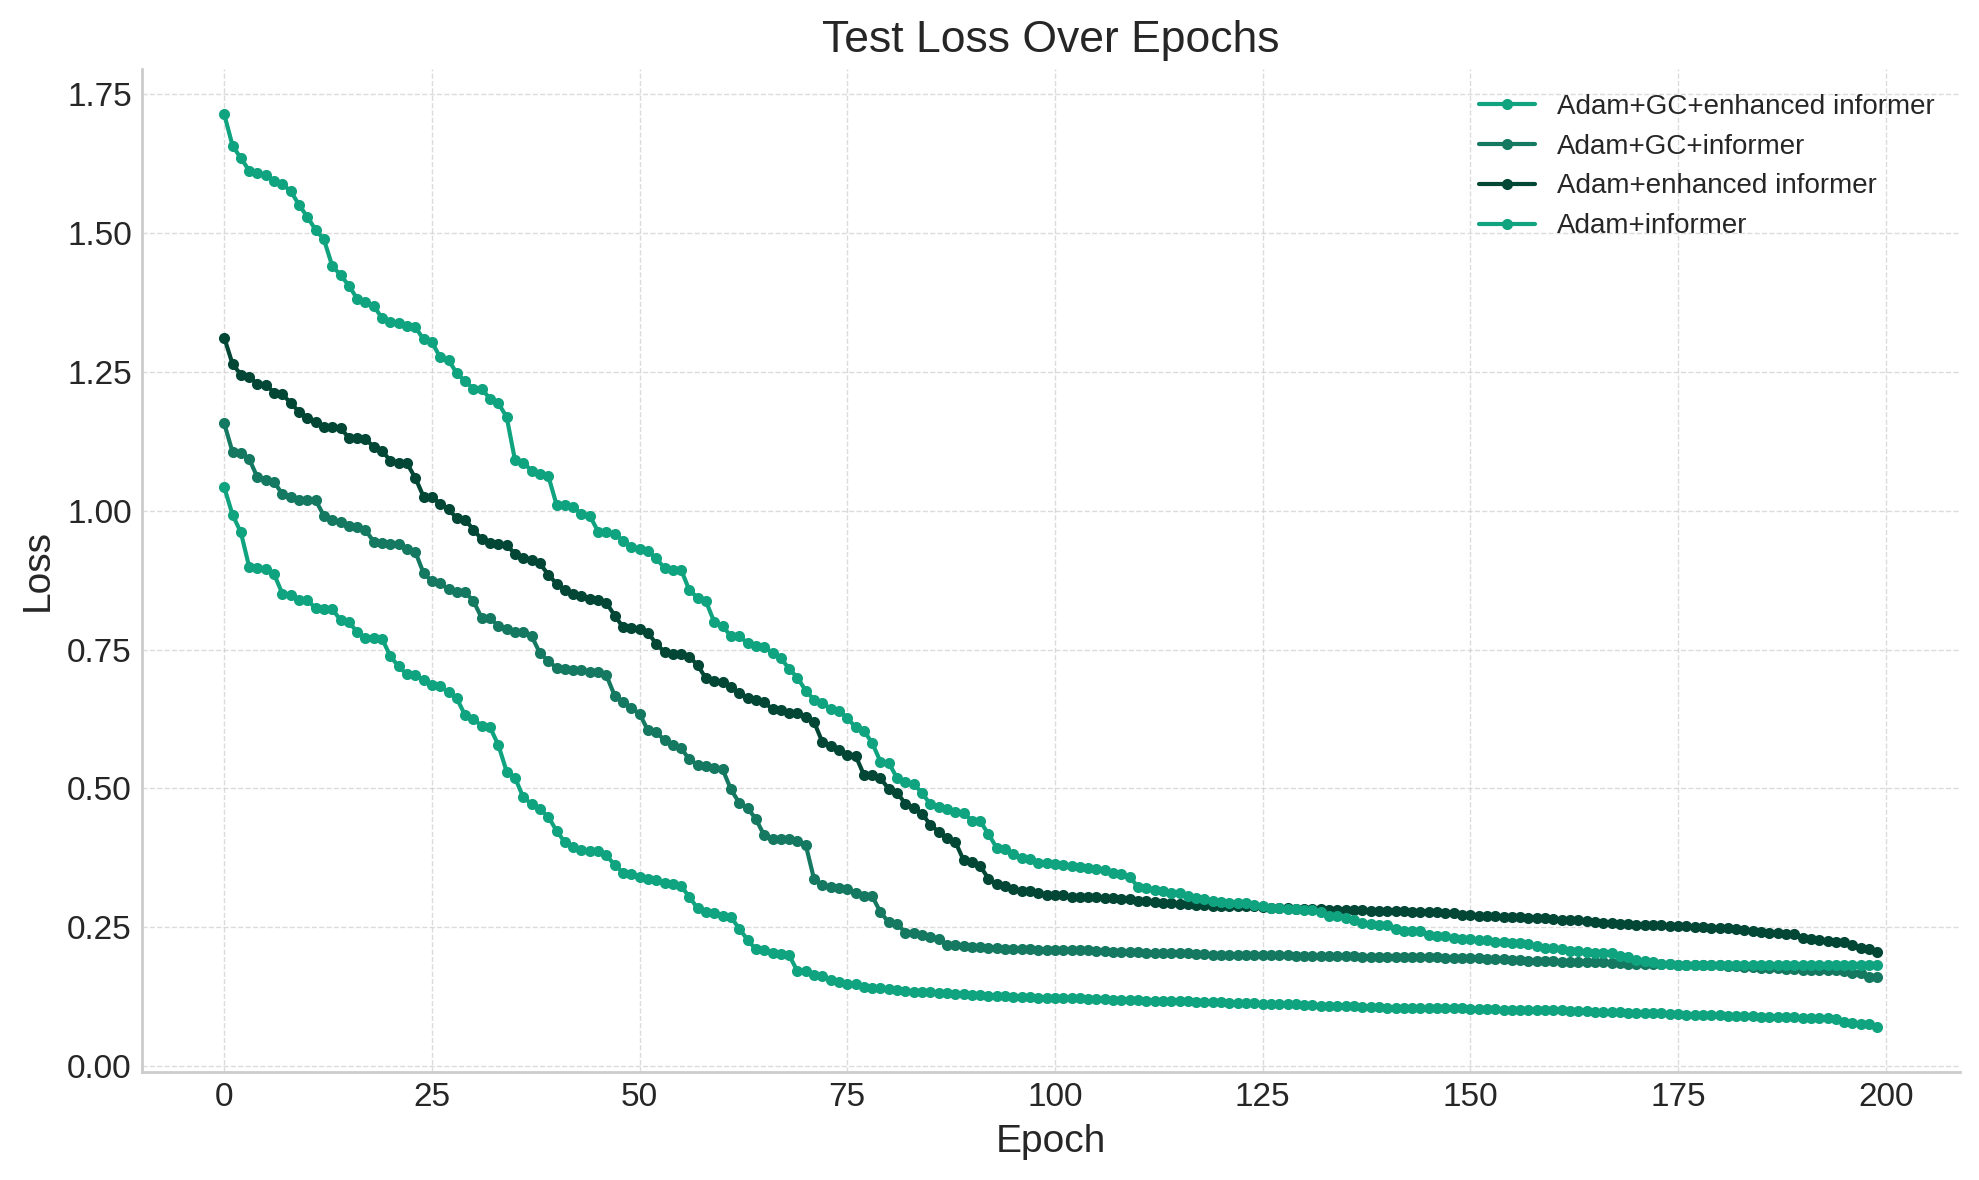
\includegraphics[width=0.7\textwidth]{pngs/loss.png}
    \caption{ Traning Results For Each Model}
    \label{loss}
\end{figure}

Within the prediction results of the ten features, the Adam+GC+enhanced informer demonstrated superior performance in terms of accuracy and robustness against drastic feature value fluctuations, as illustrated in Fig. \ref{features}.
\begin{figure}[h]
    \centering
    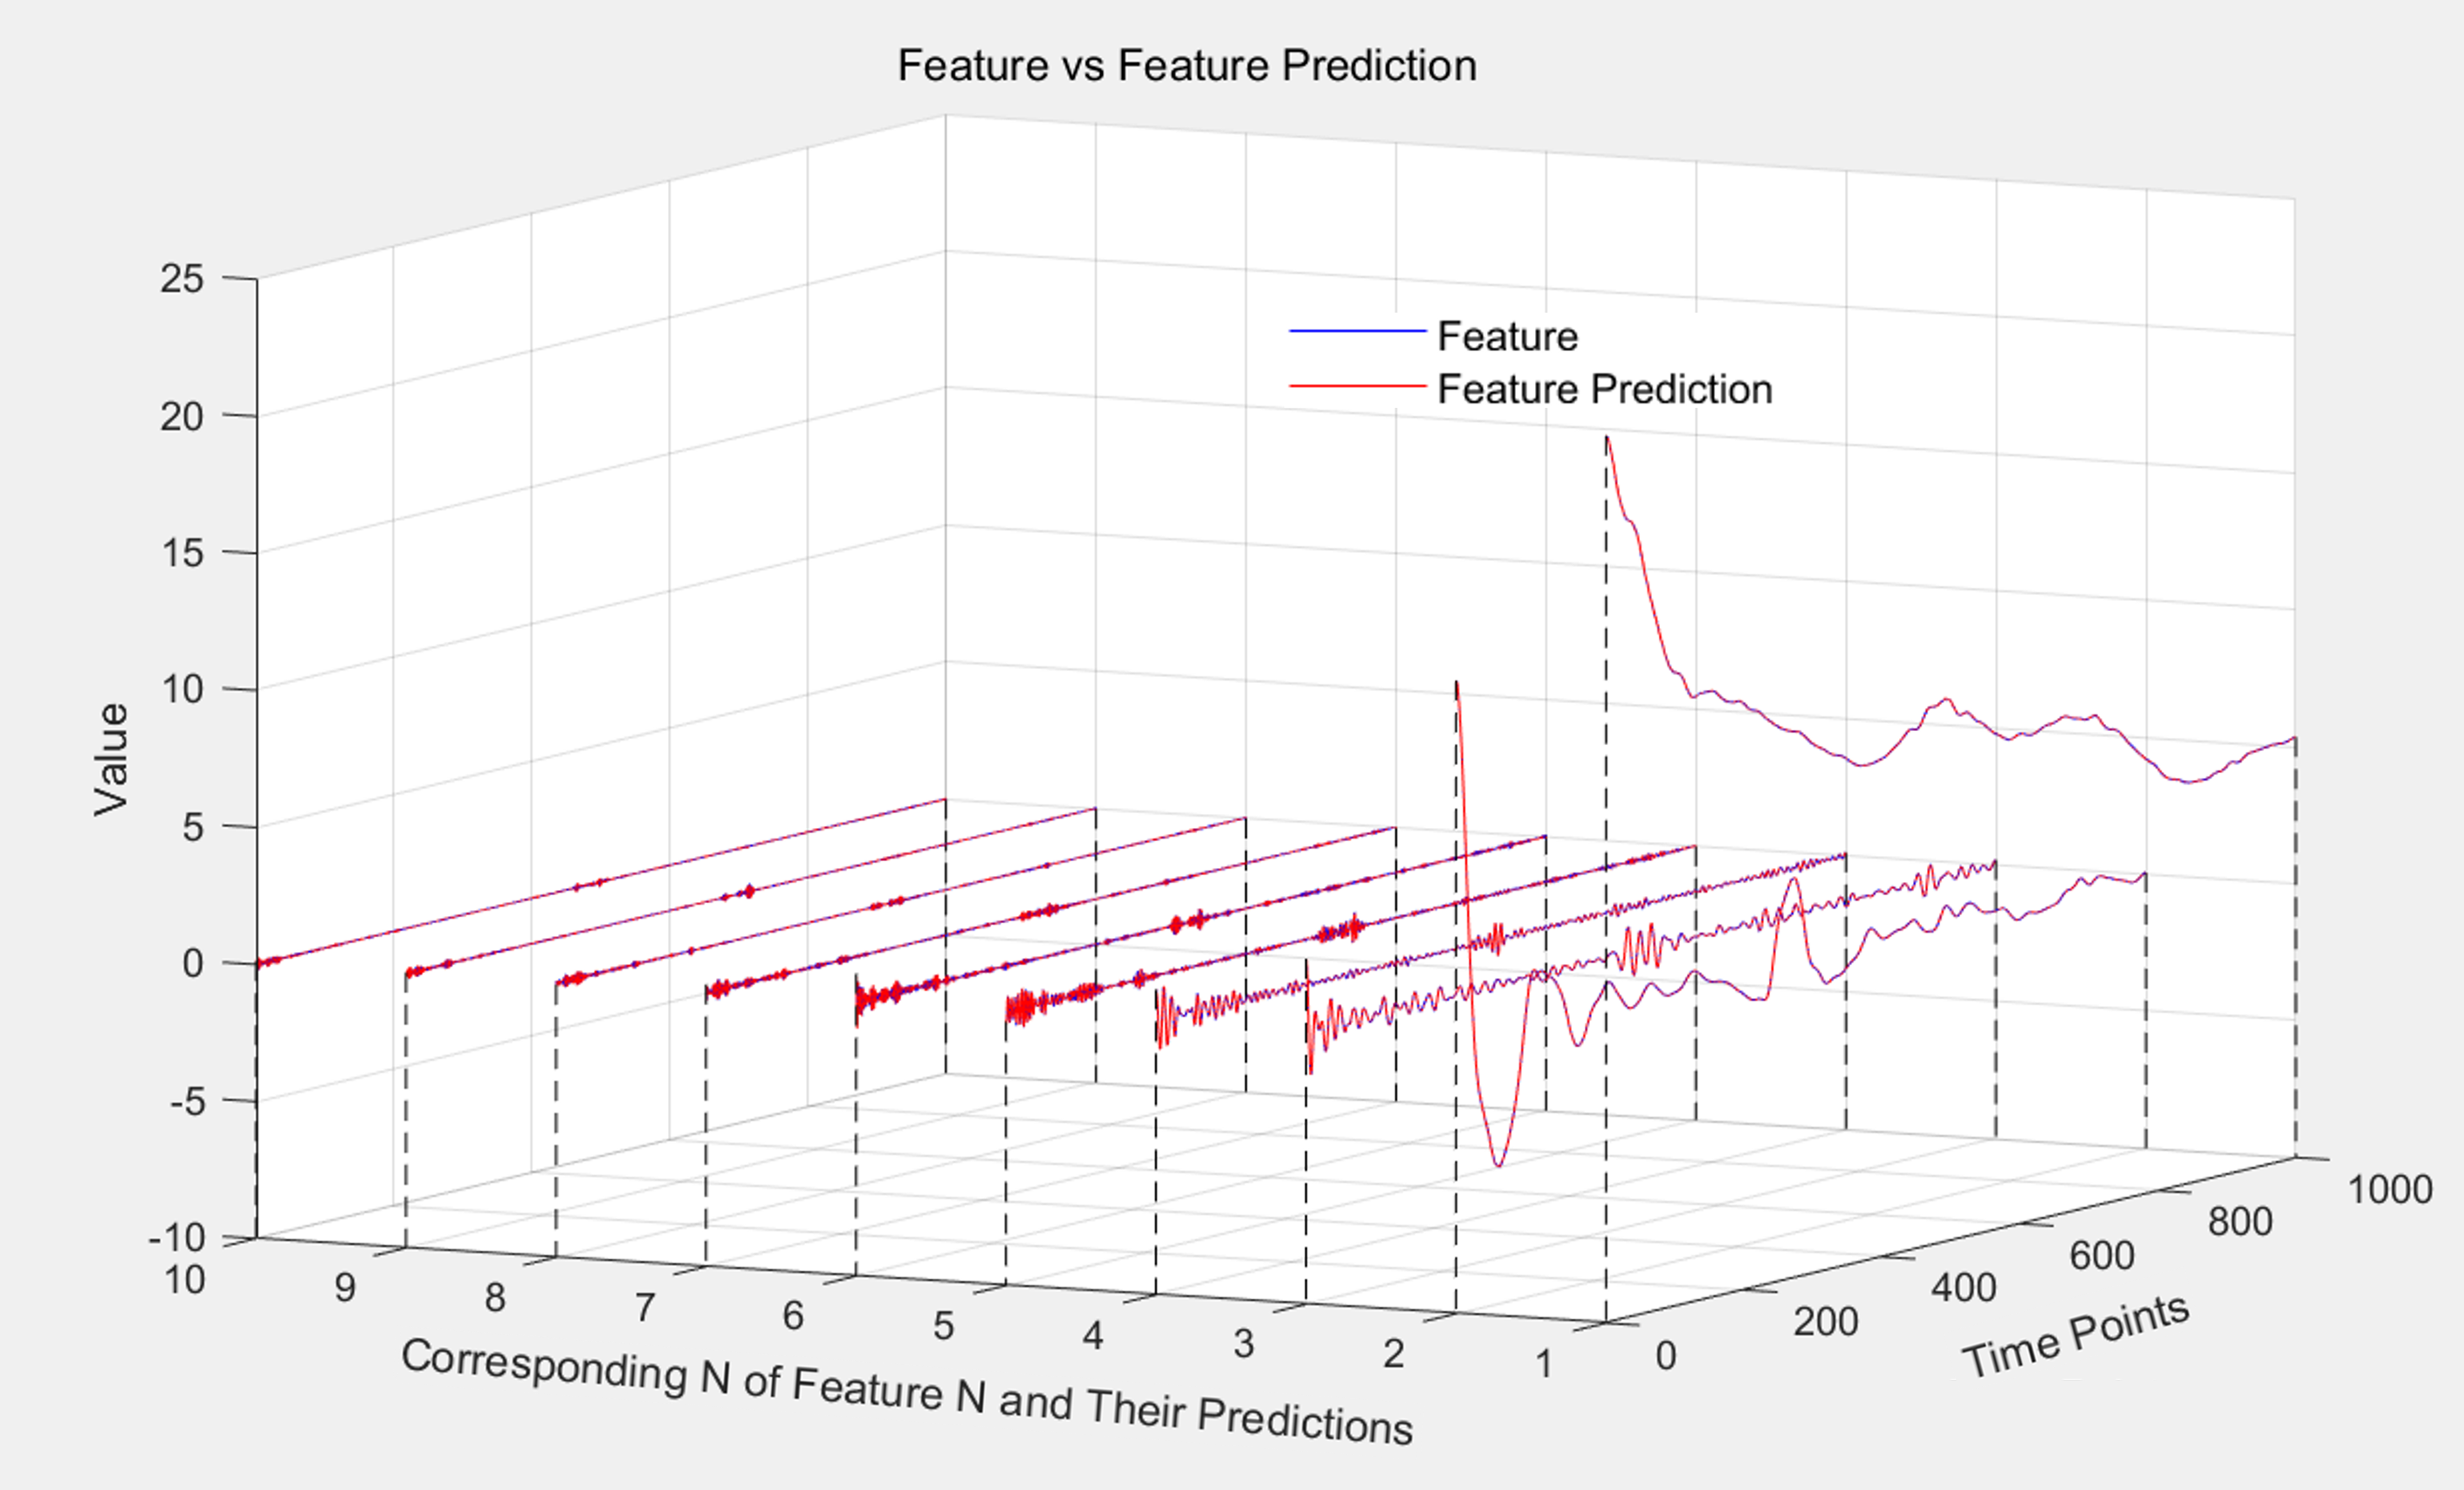
\includegraphics[width=1\textwidth]{pngs/features.png}
    \caption{ Prediction Results For Each Feature}
    \label{features}
\end{figure}
In the endeavor to predict the four financial indicators: "open", "low", "high", and "close", and to visually represent the outcomes, a comprehensive portrayal of the model's predictive prowess was imperative. To this end, all data points in the results were uniformly divided into 200 segments, chronologically, with each segment comprising 89 data points. A single data point was randomly selected from each segment to ensure a representative sample of the dataset's overall characteristics. Utilizing this methodology, the ablation study results for the "open" indicator, based on four distinct models, are displayed on the left side of Fig. \ref{disso}. Moreover, for time intervals in the overall results exhibiting significant fluctuations, a similar visualization strategy was employed, partitioning them into 200 segments, as shown on the right side of Fig. \ref{disso}.

\begin{figure}[h]
    \centering
    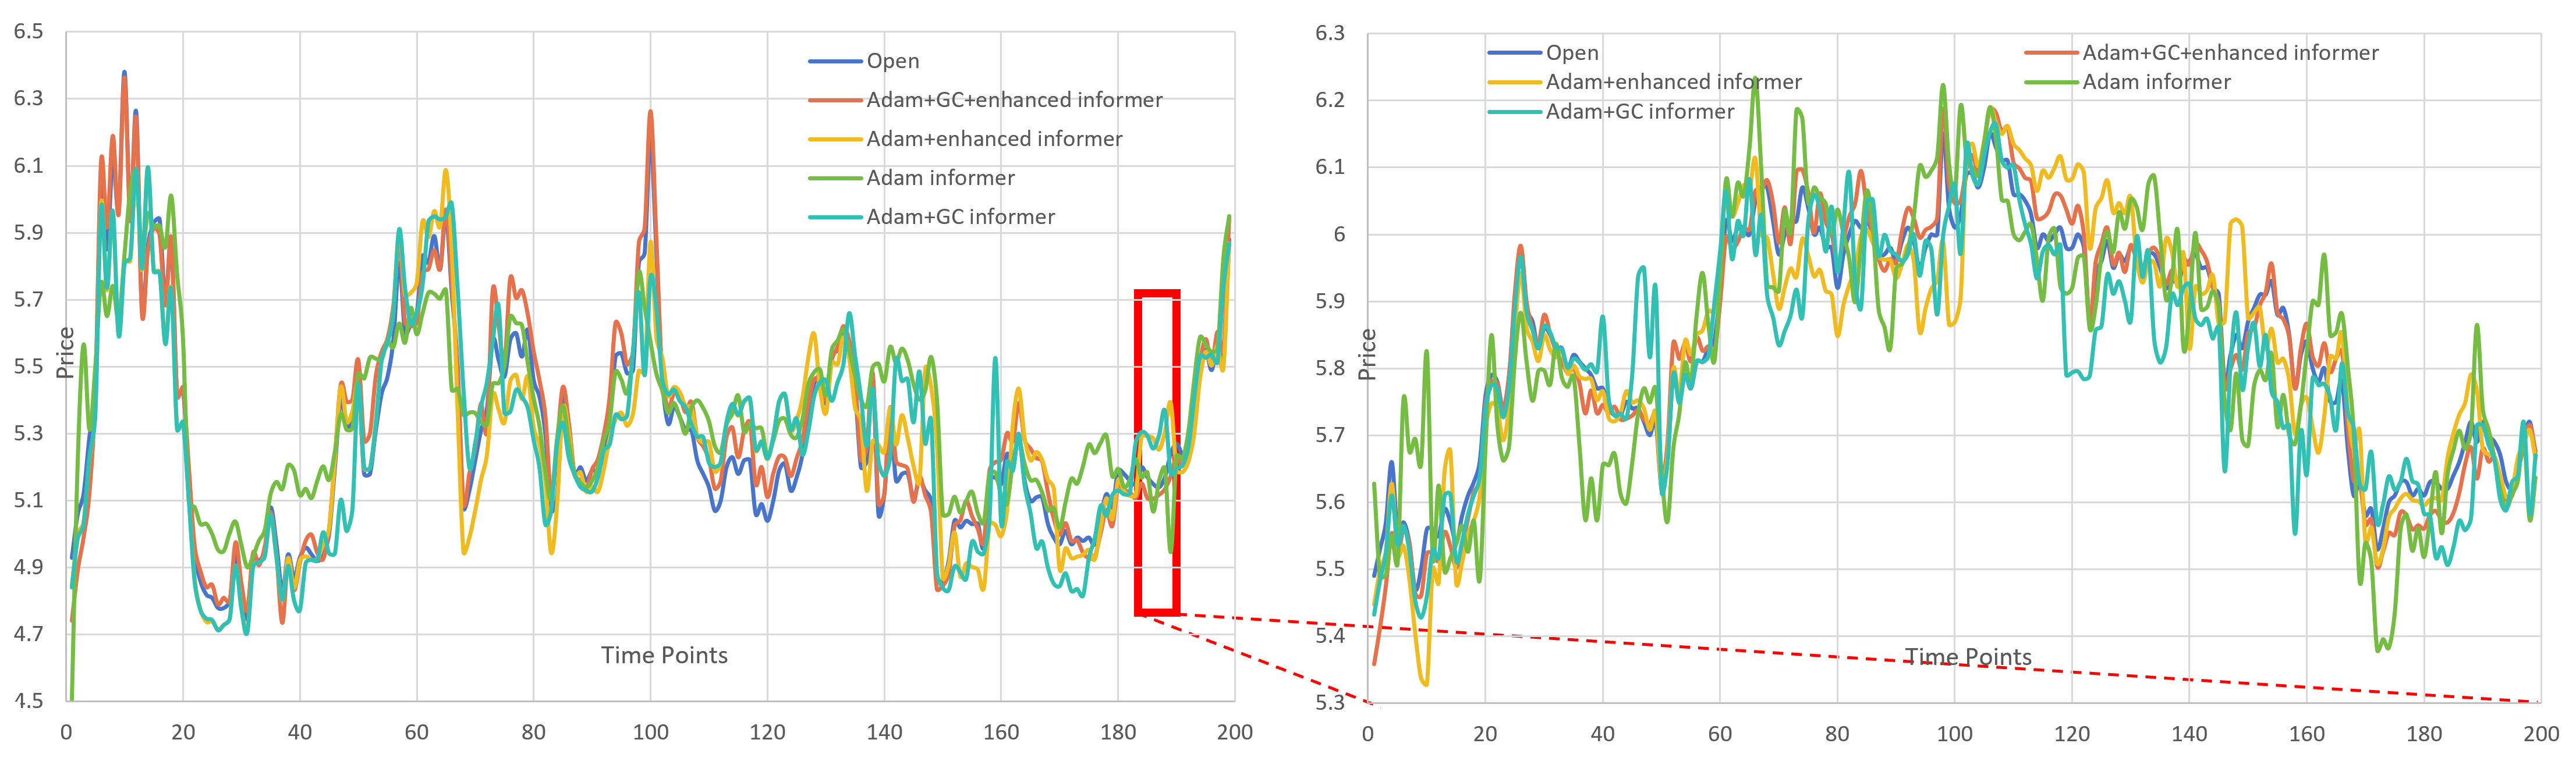
\includegraphics[width=1\textwidth]{pngs/disso.png}
    \caption{Visualized Results of Ablation Experiments}
    \label{disso}
\end{figure}

To accentuate the disparities in predictive outcomes across the models, individual model predictions were also distinctly presented. Fig. \ref{disso_all} delineates the predictions from all four models across the entire time frame, while Fig. \ref{disso_part} showcases their respective predictions during periods of pronounced changes.

\begin{figure}[h]
    \centering
    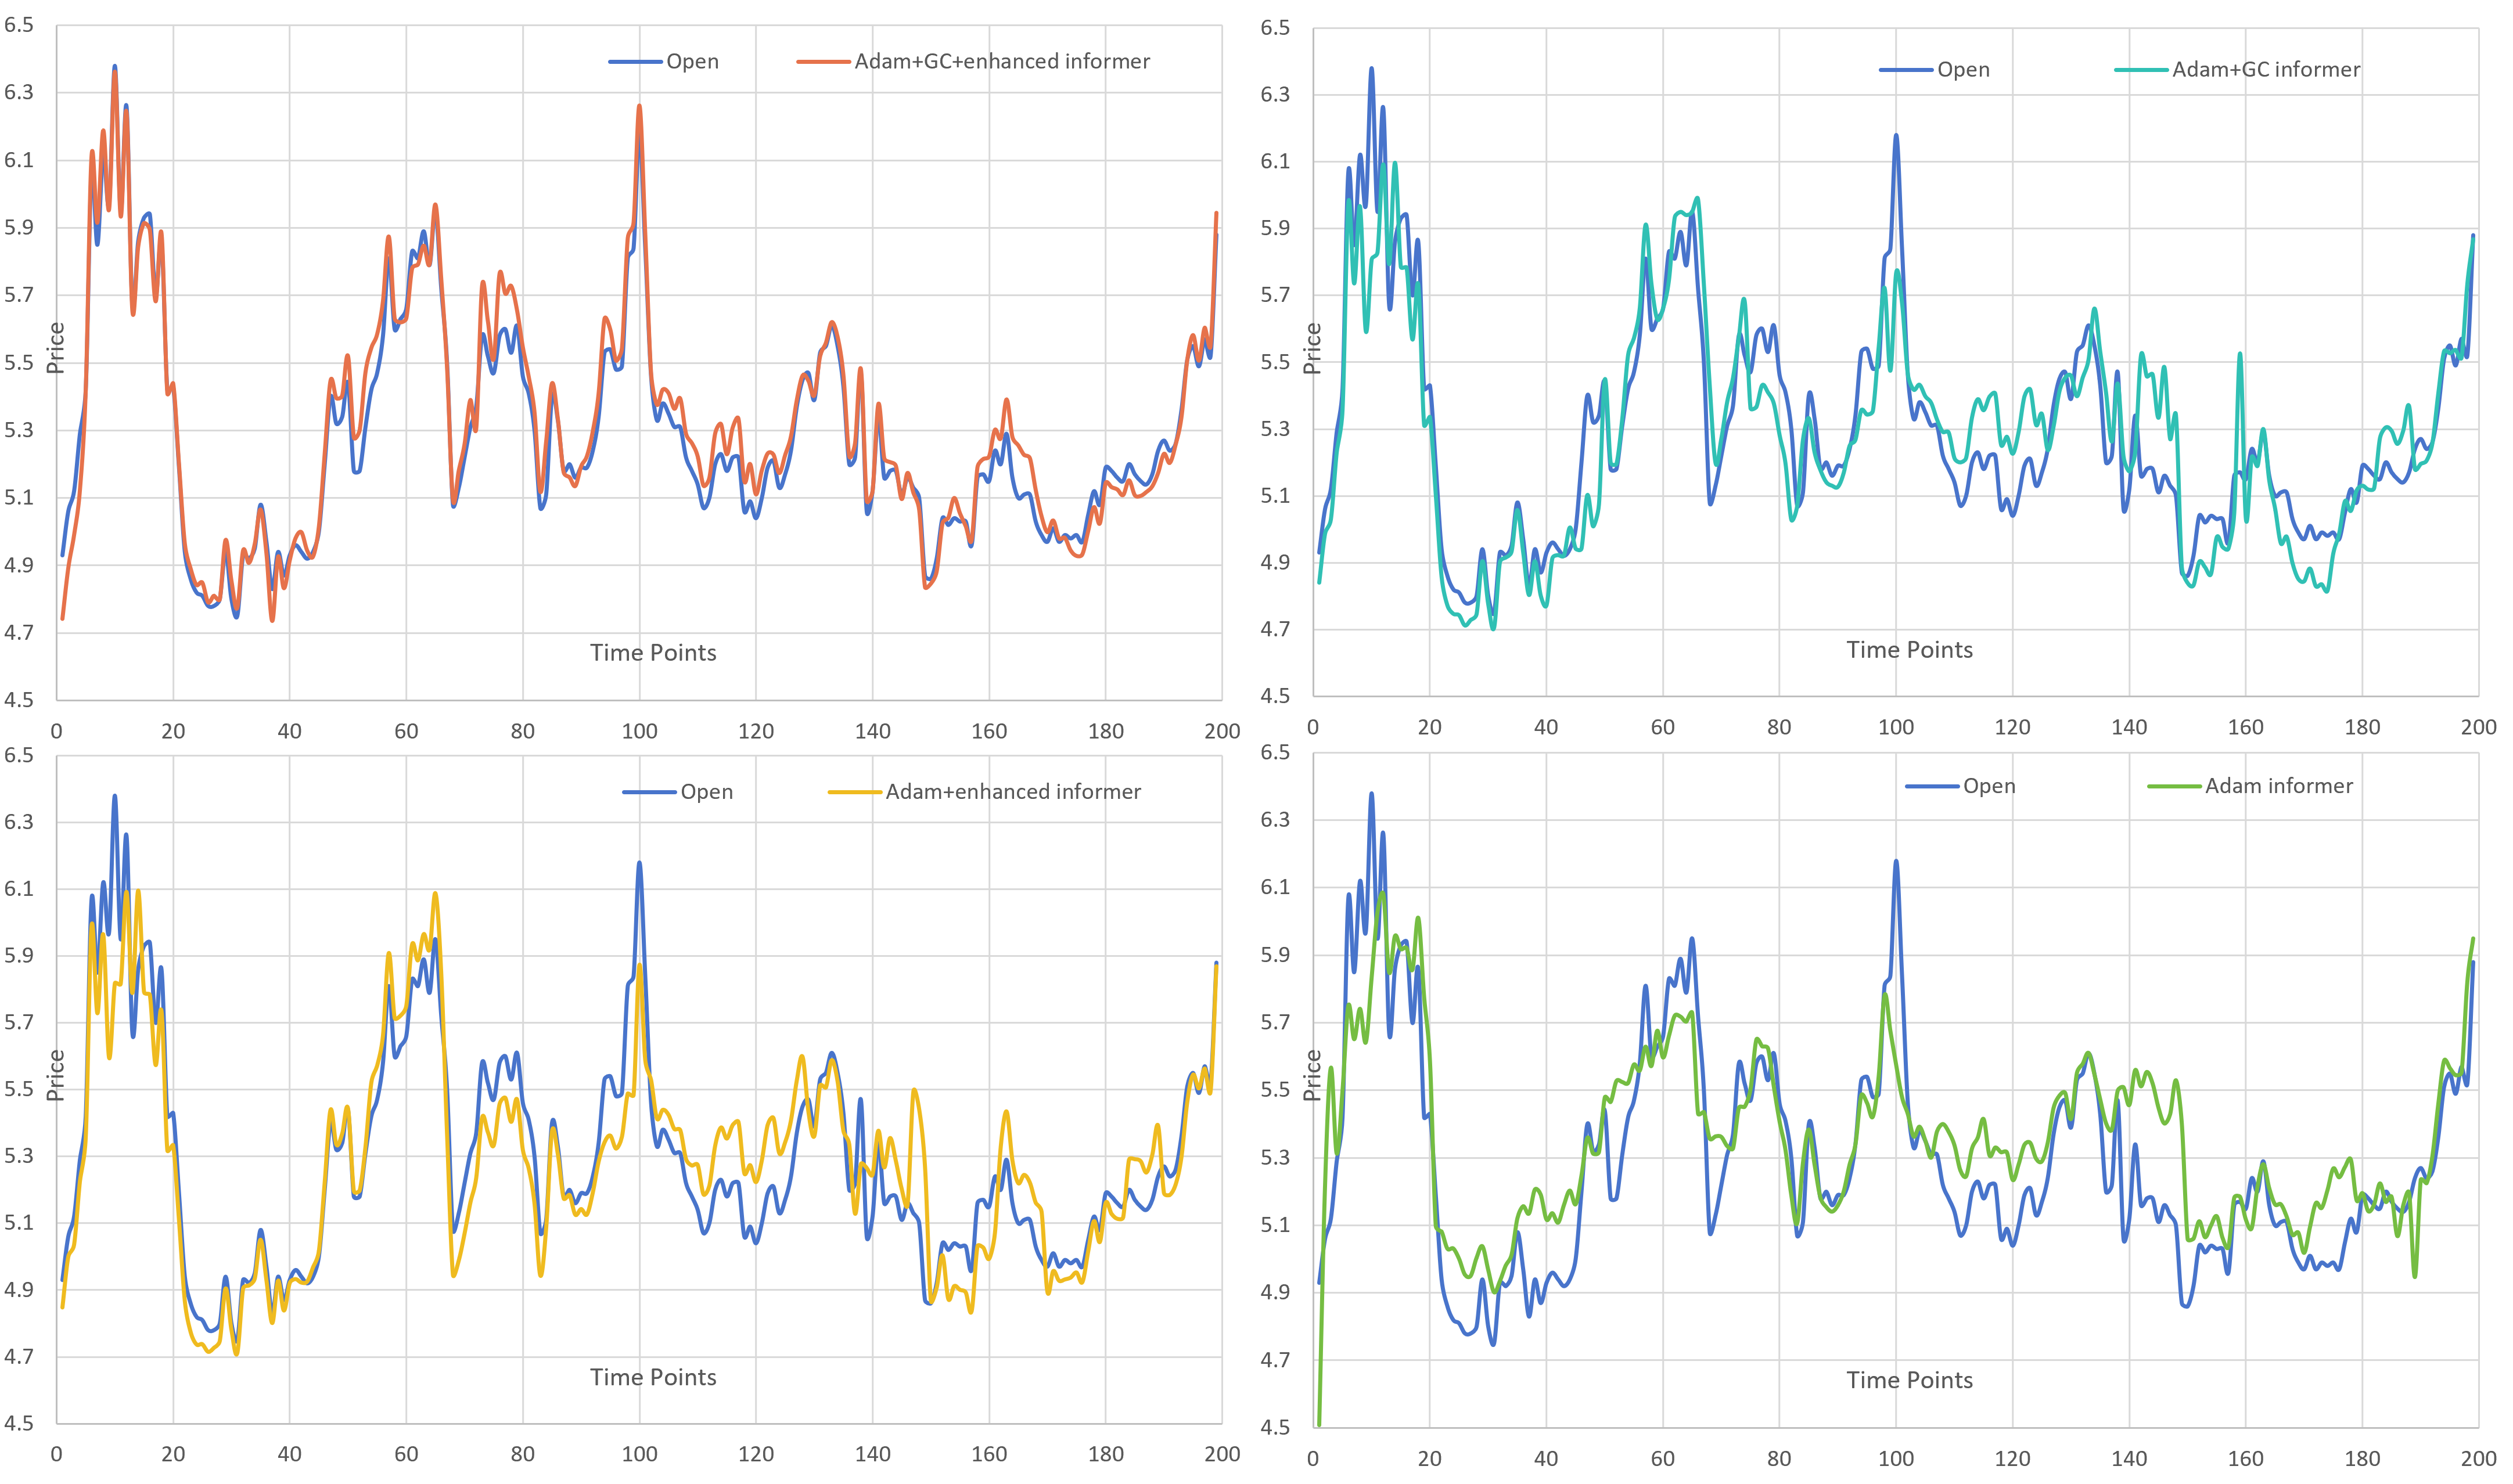
\includegraphics[width=1\textwidth]{pngs/disso_all.png}
    \caption{ Visualized Results of Ablation Experiments for Individual Model: Overall Time Frame}
    \label{disso_all}
\end{figure}

\begin{figure}[h]
    \centering
    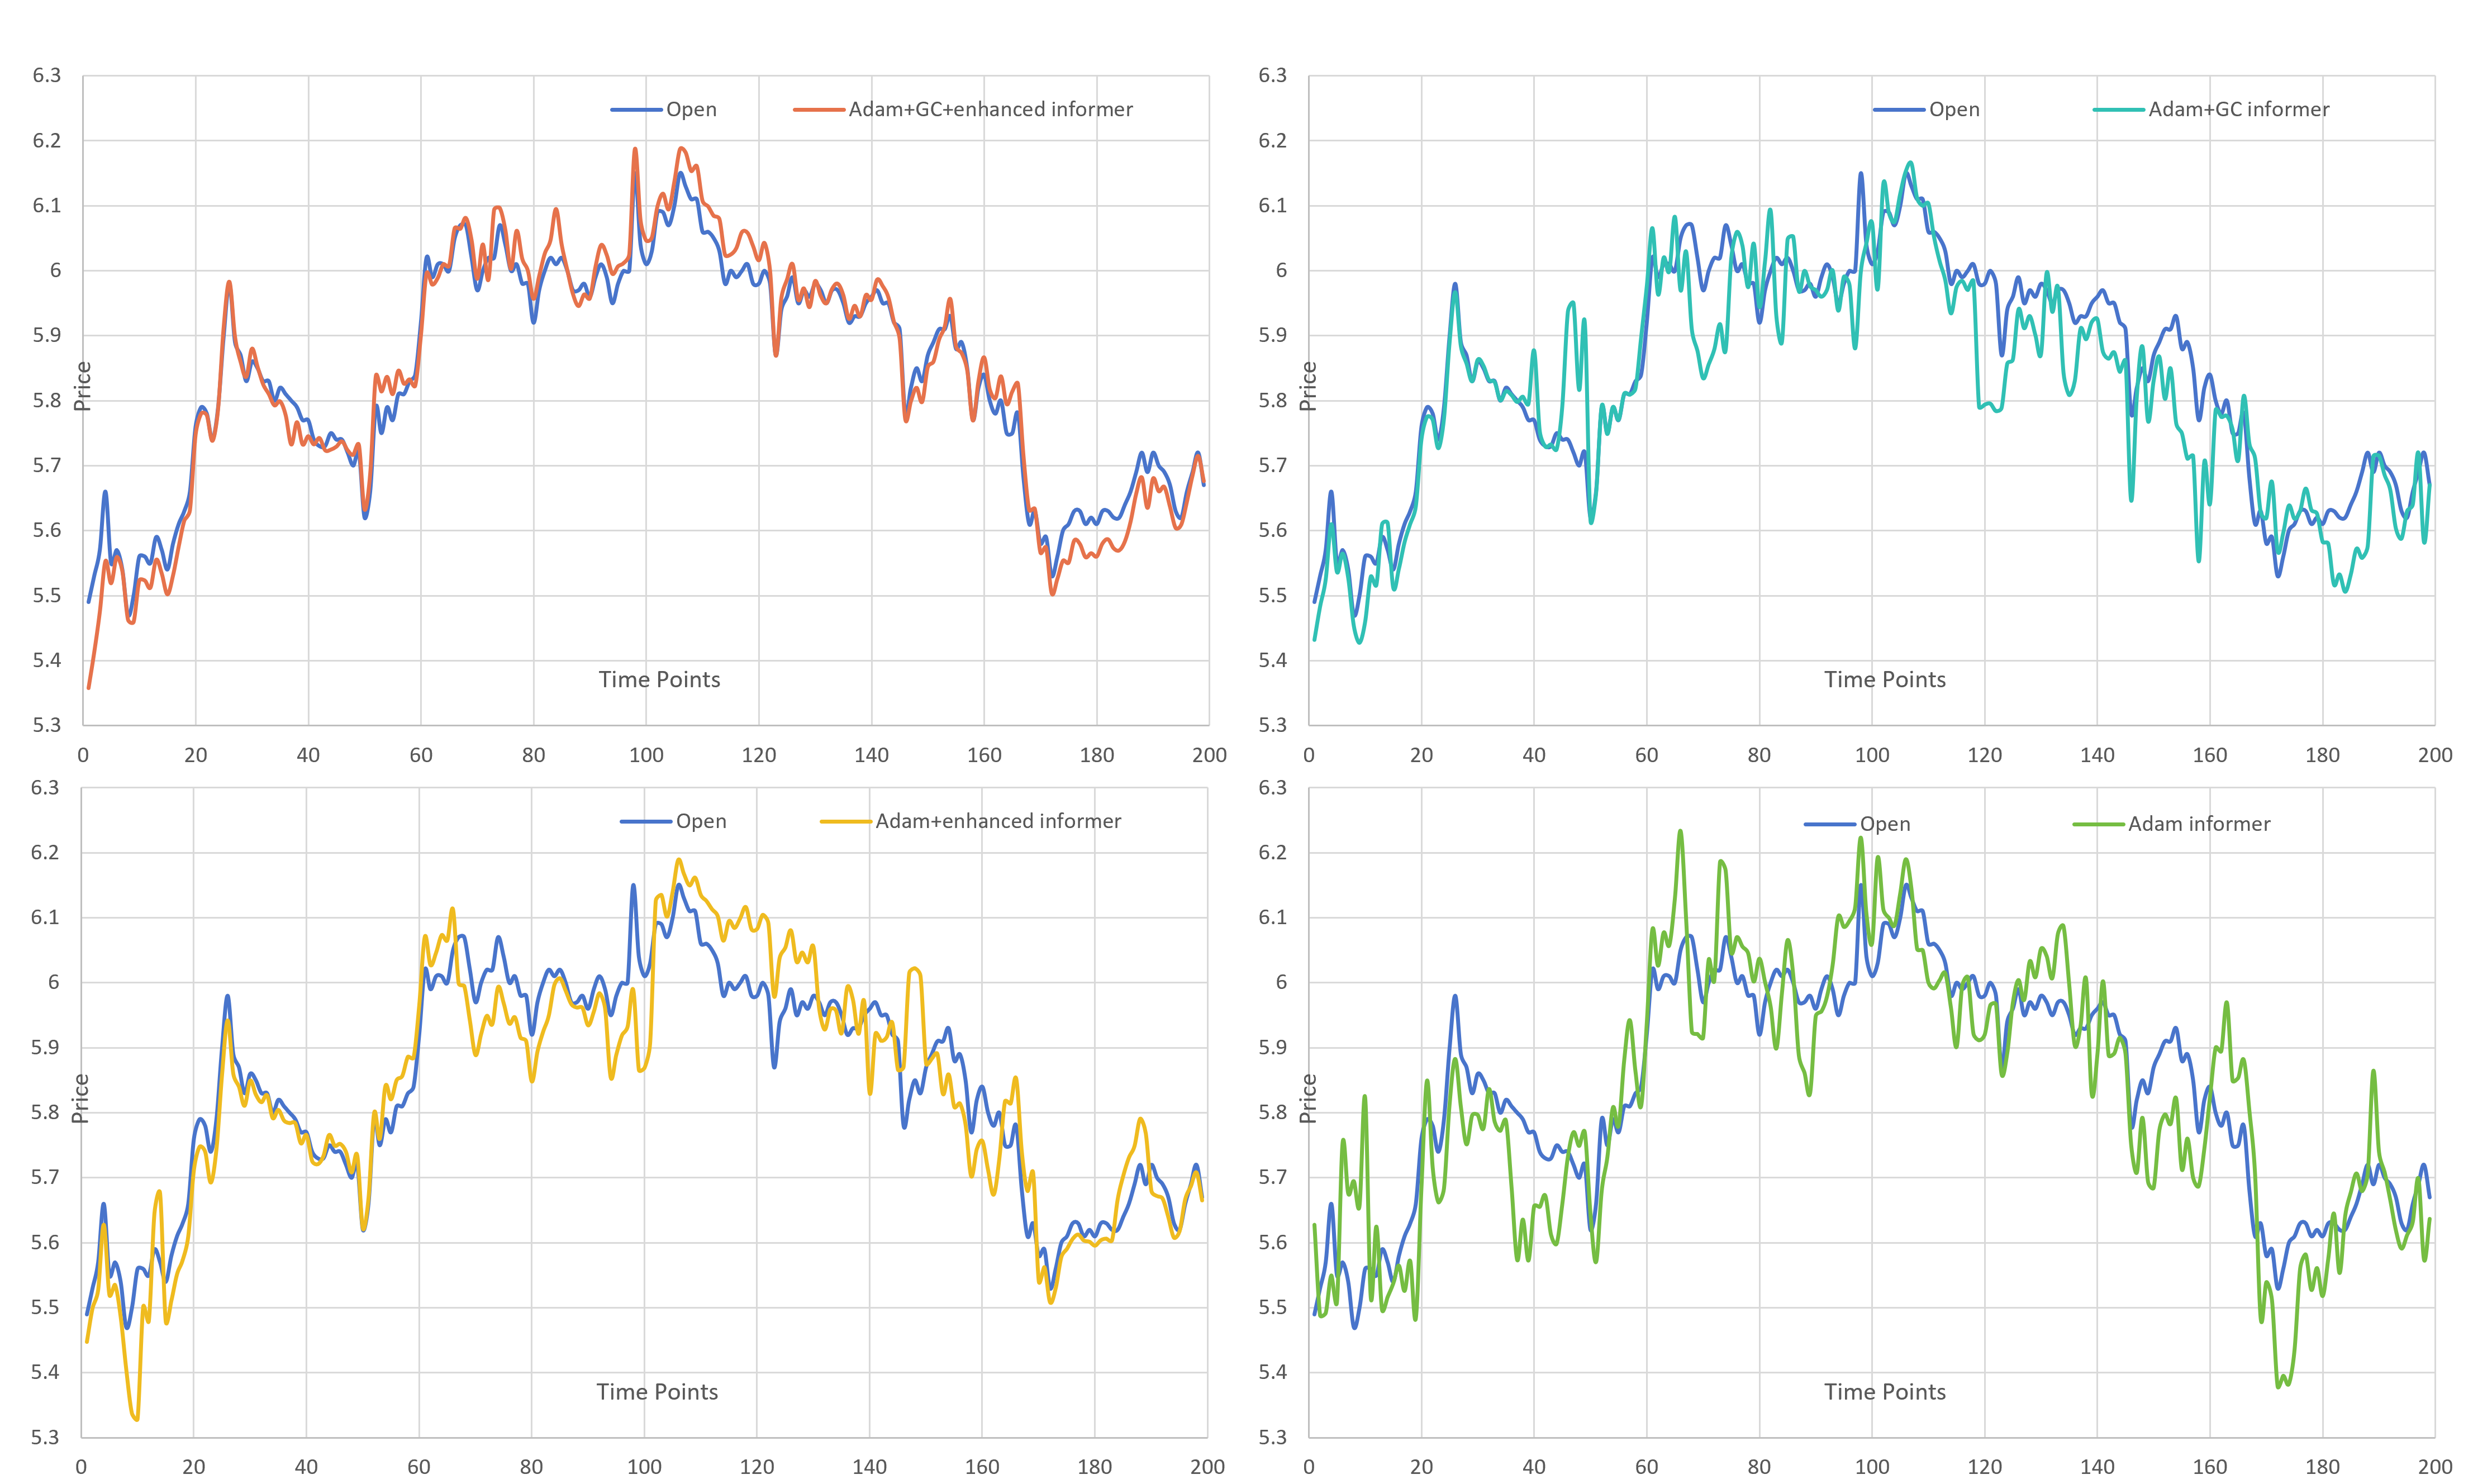
\includegraphics[width=1\textwidth]{pngs/disso_part.png}
    \caption{ Visualized Results of Ablation Experiments for Individual Model: Volatile Time Frame}
    \label{disso_part}
\end{figure}

Based on the visualization of the prediction results and in conjunction with the training times and errors presented in Table \ref{error_disso} for different models, we can draw the following analysis:

\begin{itemize}
\item \textbf{Advantages of the Adaptive Function}:
When predicting the dynamic changes in the financial market, inflection points often pose significant challenges. In this regard, the Adam-GC Informer model exhibited a pronounced accuracy over the Adam-Informer model. This observation underscores the effectiveness of the introduced adaptive function in mitigating errors and uncertainties at abrupt market shifts.
\item \textbf{GC Data Processing and Temporal Lag}:
Data handling and preprocessing stand as pivotal steps in the predictive pipeline. Our evaluations reveal that by employing the Adam+GC+enhanced model, predictions align more closely with actual market data, emphasizing the role of data processing techniques in mitigating temporal lags in predictions.
\item \textbf{Training Efficiency and Loss Function}:
An efficacious loss function is pivotal in ensuring model training efficiency and accuracy. The introduction of an adaptive loss function facilitated a noticeable reduction in training time for the Adam-GC Informer model, simultaneously bolstering its robustness and predictive fidelity.
\item \textbf{Performance Evaluation of the Hybrid Model}:
The hybrid model introduced in this study exhibited commendable performance across various assessment metrics. In comparison to the Adam-Informer, Adam+enhanced, and Adam+GC informer models, the hybrid model manifested a substantial improvement in MAE, with reductions of 63.15\%, 55.86\%, and 62.59\% respectively. Furthermore, it also demonstrated reductions in RMSE by 57.71\% and 30.7\% respectively, while showcasing enhancements in $R^2$ values by 13.75\%, 17.60\%, and 29.37\% respectively.
\end{itemize}

Upon contrasting various models, it becomes evident that the Adam+GC+enhanced model possesses the capability to decompose raw stock data into finer granules, thereby delving deeper into the intrinsic dynamics and features of stocks. This intricate exploration furnishes financial decision-makers with predictions that are both precise and timely.

\begin{table}[h]
\caption{Forecasting Errors of Different Models in Ablation Experiment}\label{error_disso}%
\centering
\begin{tabular}{@{}ccccc@{}}
\toprule
\textbf{Model} & \textbf{MAE}& \textbf{RMSE}& \textbf{$R^2$} & \textbf{Time(s)}\\
\midrule
Adam+GC+enhanced informer & 0.049 & 0.063 & 0.960 & 1237.39 \\
Adam+GC informer & 0.102 & 0.091 & 0.828 & 1026.94 \\
Adam+enhanced informer & 0.111 & 0.114 & 0.791 & 1543.84 \\
Adam+informer & 0.133 & 0.149 & 0.678 & 1836.41 \\
\bottomrule
\end{tabular}
\end{table}


\subsubsection{Comparative Experiment}\label{subsubsec2}

To rigorously assess the overall superiority of the proposed model, we benchmarked against traditional models including Informer, LSTM, ANN, and CNN, all under parameter settings consistent with VMGCformer. The prediction outcomes are depicted in Fig. \ref{comp_single}. In addition, we further compared our model with other hybrid models like EMD-FE-Informer, IVMD-F-Informer, and CNNInformer, with results presented in Fig. \ref{comp_mix}. And the error values for the predictions of all models can be found in Table \ref{error_comp}.The box plot of prediction errors for selected models compared to VMGCforme is depicted in Fig. \ref{case}. It is evident that VMGCforme outperforms other models in terms of training error, and it converges more rapidly to a stable level.

\begin{figure}[h]
    \centering
    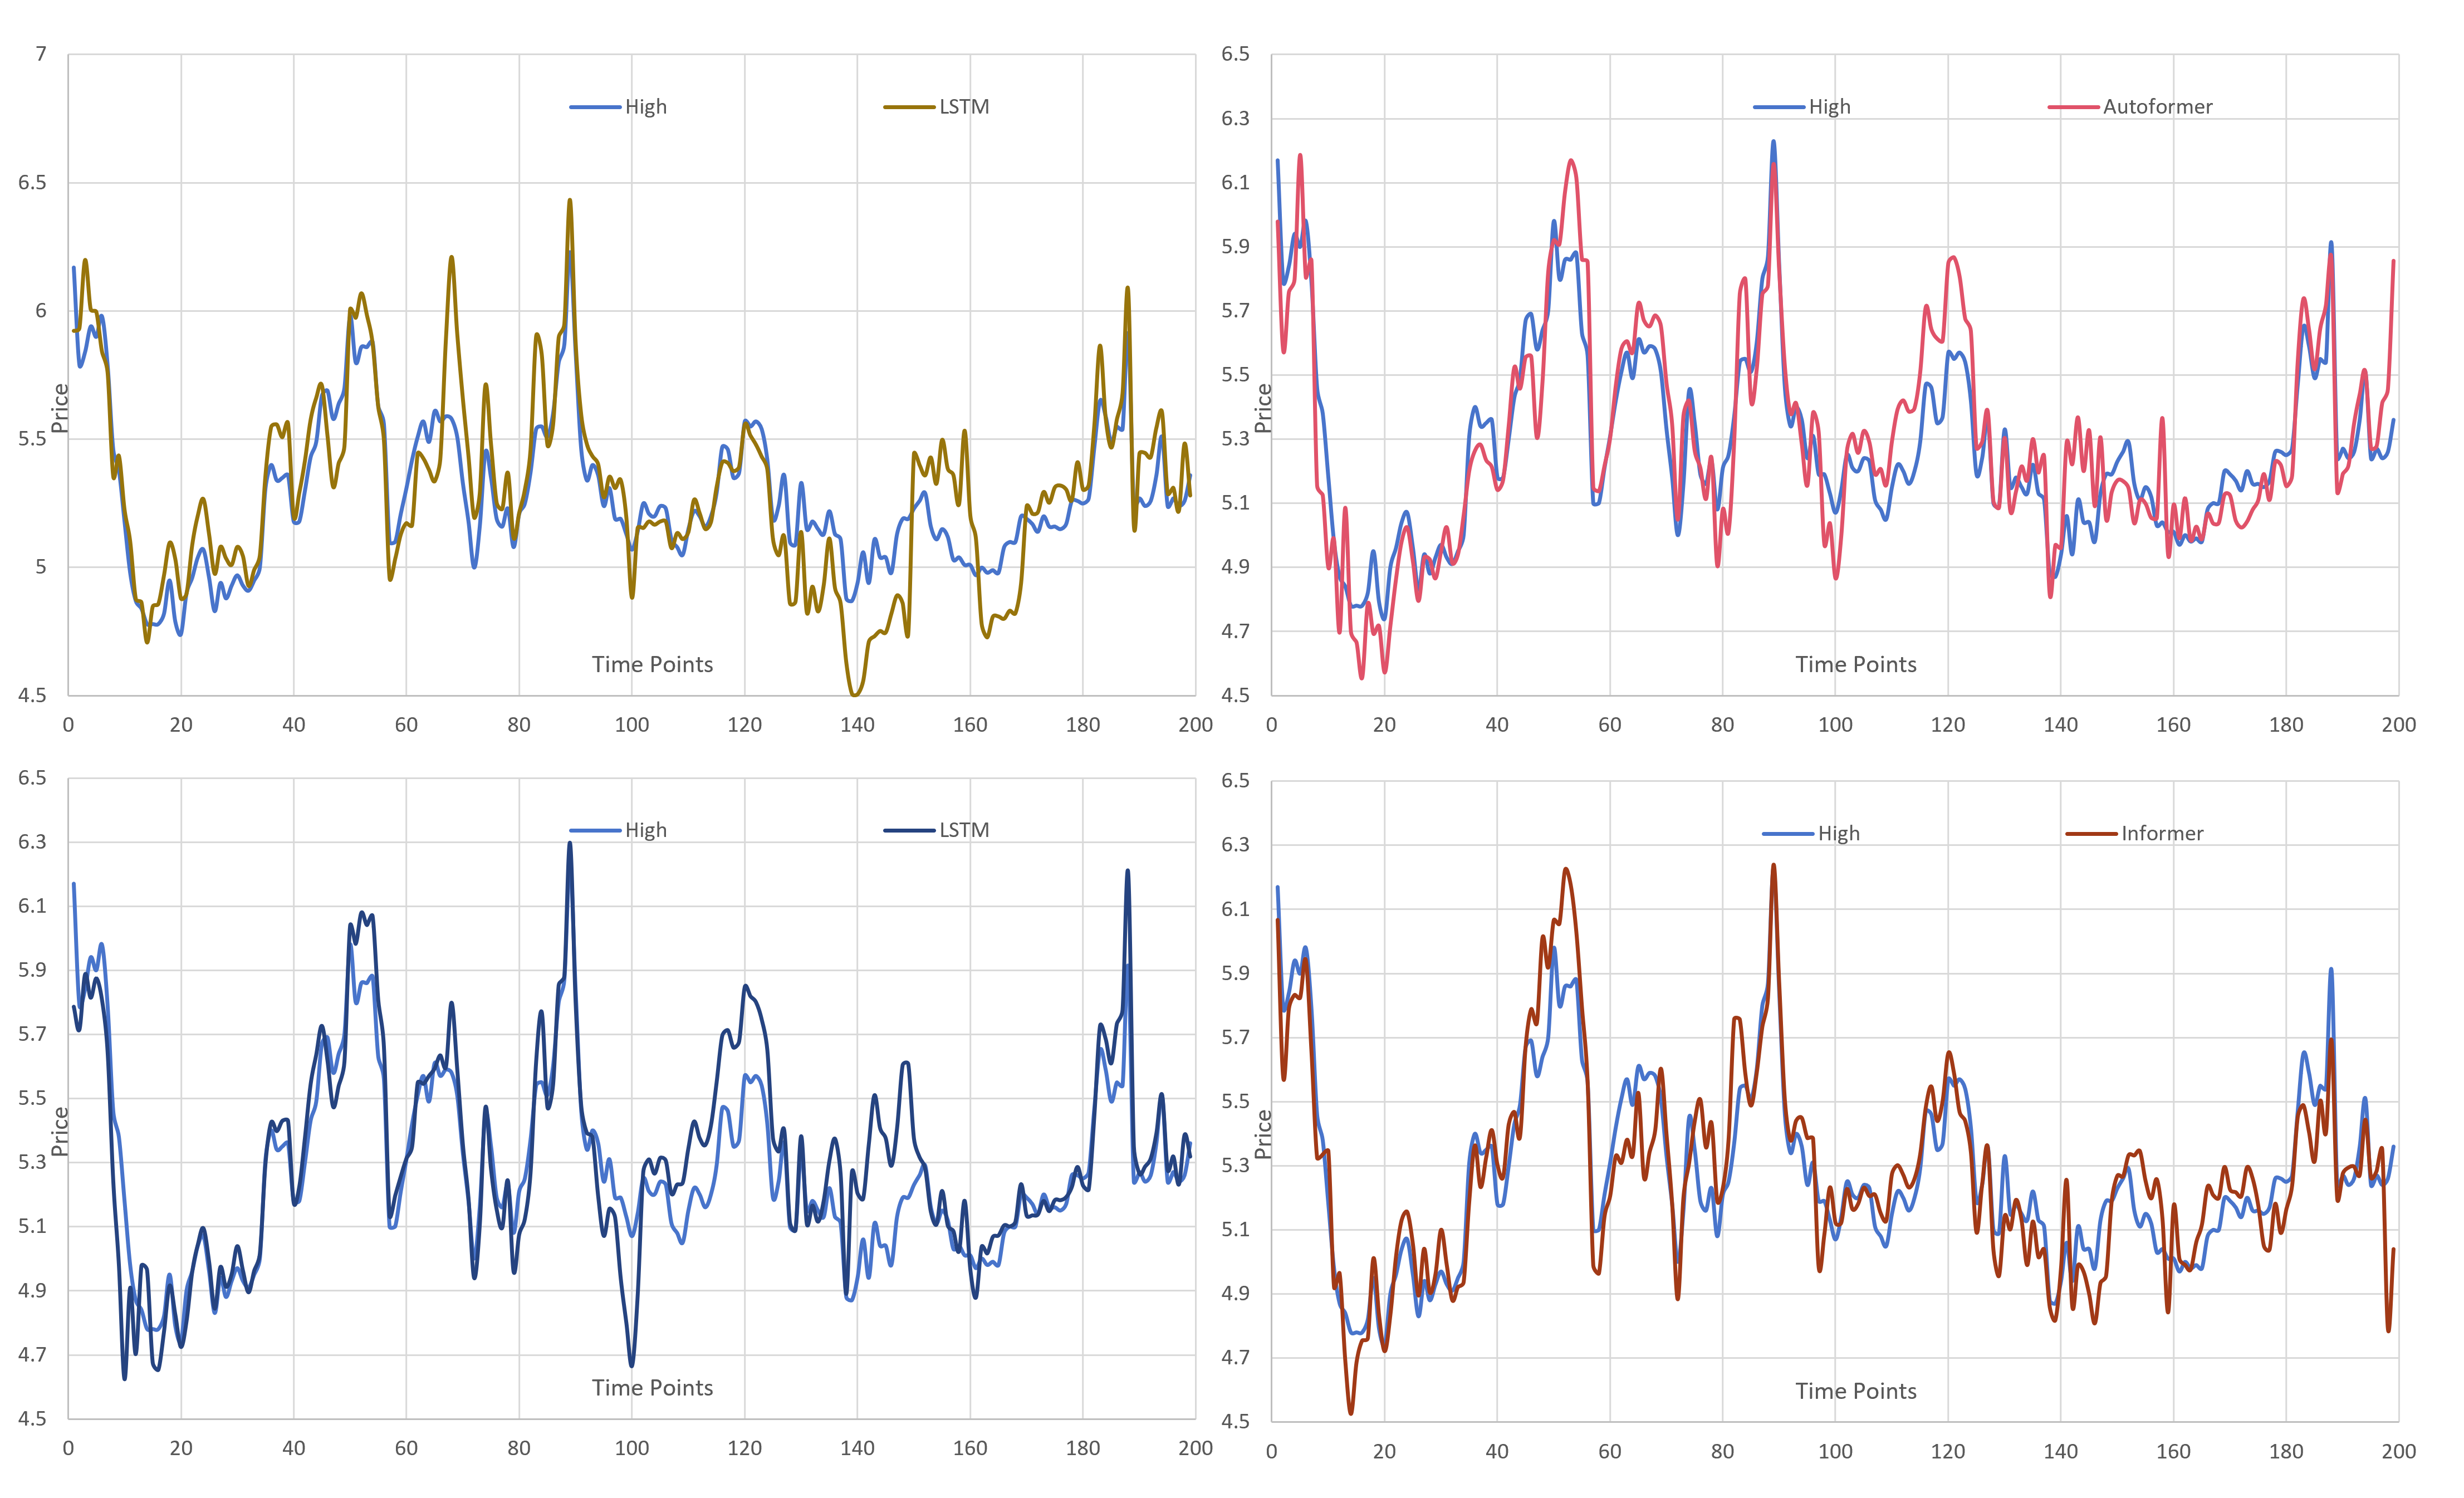
\includegraphics[width=1\textwidth]{pngs/comp_single.png}
    \caption{ Single Model Prediction Results}
    \label{comp_single}
\end{figure}

\begin{figure}[h]
    \centering
    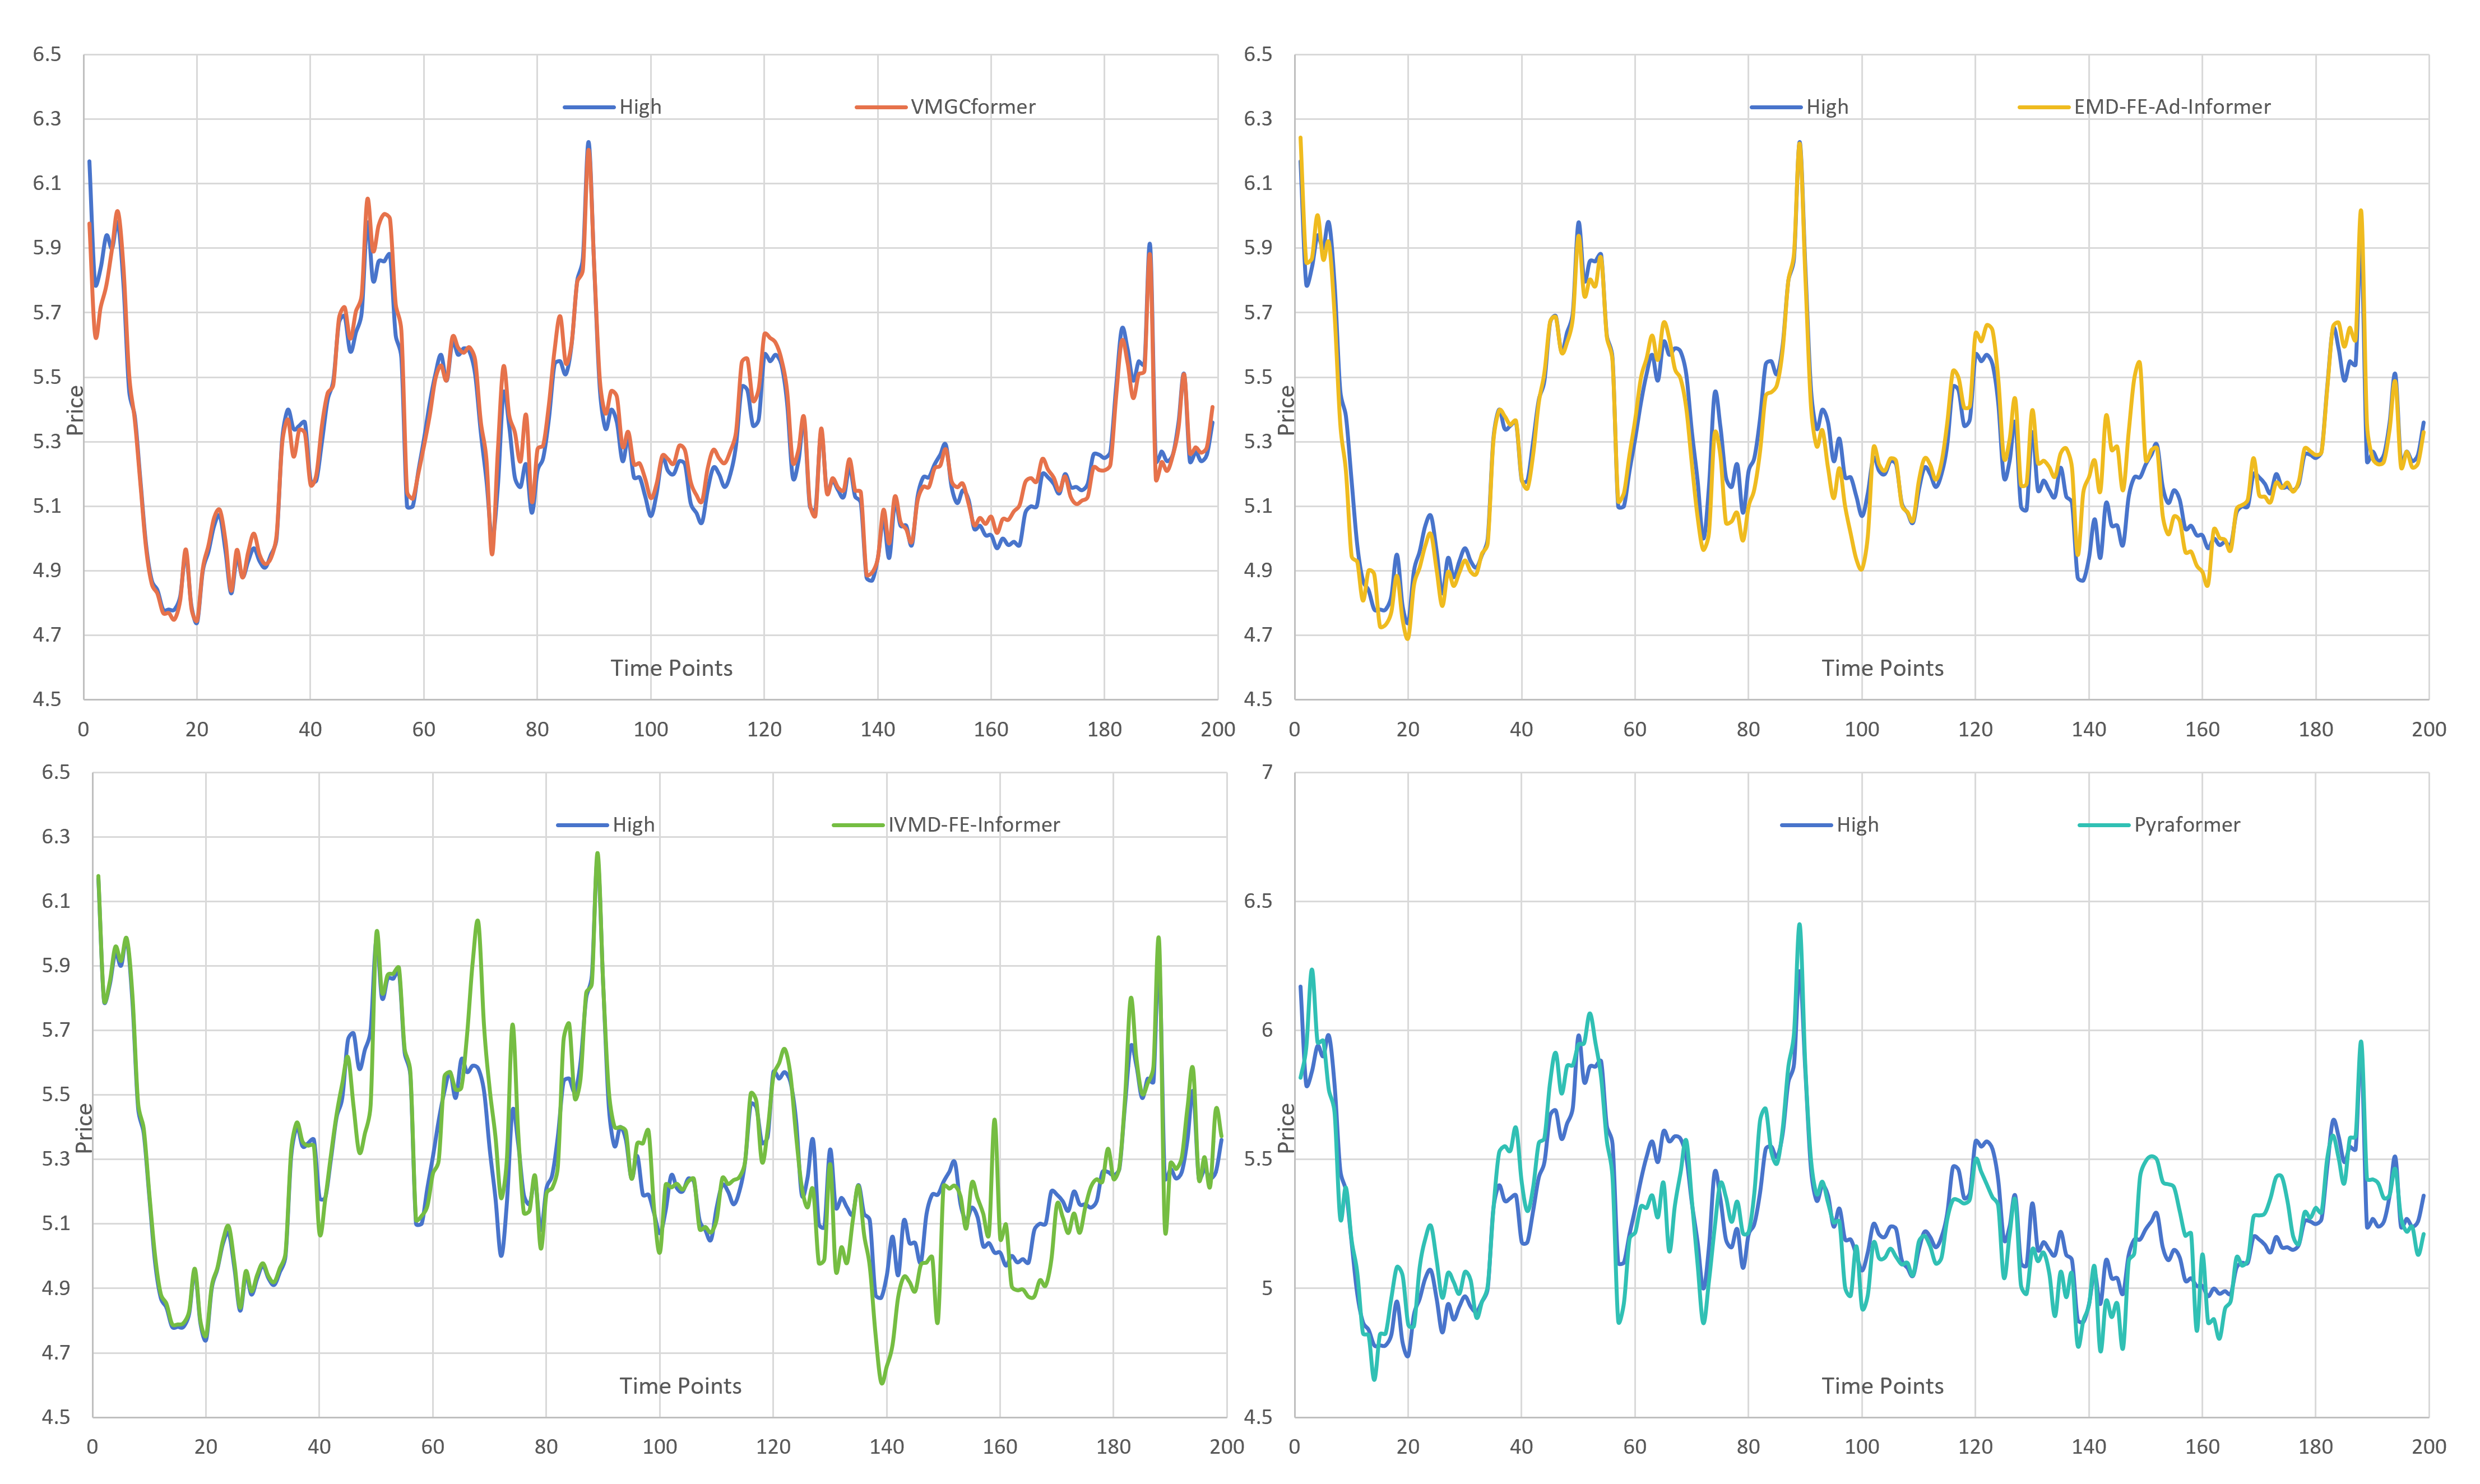
\includegraphics[width=1\textwidth]{pngs/comp_mix.png}
    \caption{ Mixture Model Prediction Results}
    \label{comp_mix}
\end{figure}

\begin{table}[h]
\caption{Forecasting Errors of Different Models in Comparative Experiment}\label{error_comp}
\centering
\begin{tabular}{@{}ccccc@{}}
\toprule
\textbf{Model} & \textbf{MAE}& \textbf{RMSE}& \textbf{\(R^2\)} & \textbf{Time(s)}\\
\midrule
VMGCformer & 0.036 & 0.053 & 0.965 & 1237.39 \\
EMD-FE-Ad-Informer & 0.066 & 0.089 & 0.902 & 1004.23 \\
Pyraformer & 0.076 & 0.108 & 0.857 & 1124.58 \\
IVMD-FE-Informer & 0.102 & 0.138 & 0.765 & 1382.24 \\
Autoformer & 0.101 & 0.148 & 0.758 & 420.25 \\
TimesNet & 0.115 & 0.153 & 0.712 & 363.14 \\
Informer & 0.124 & 0.162 & 0.678 & 143.35 \\
LSTM & 0.139 & 0.183 & 0.587 & 524.35 \\
\bottomrule
\end{tabular}
\end{table}

\begin{figure}[h]
    \centering
    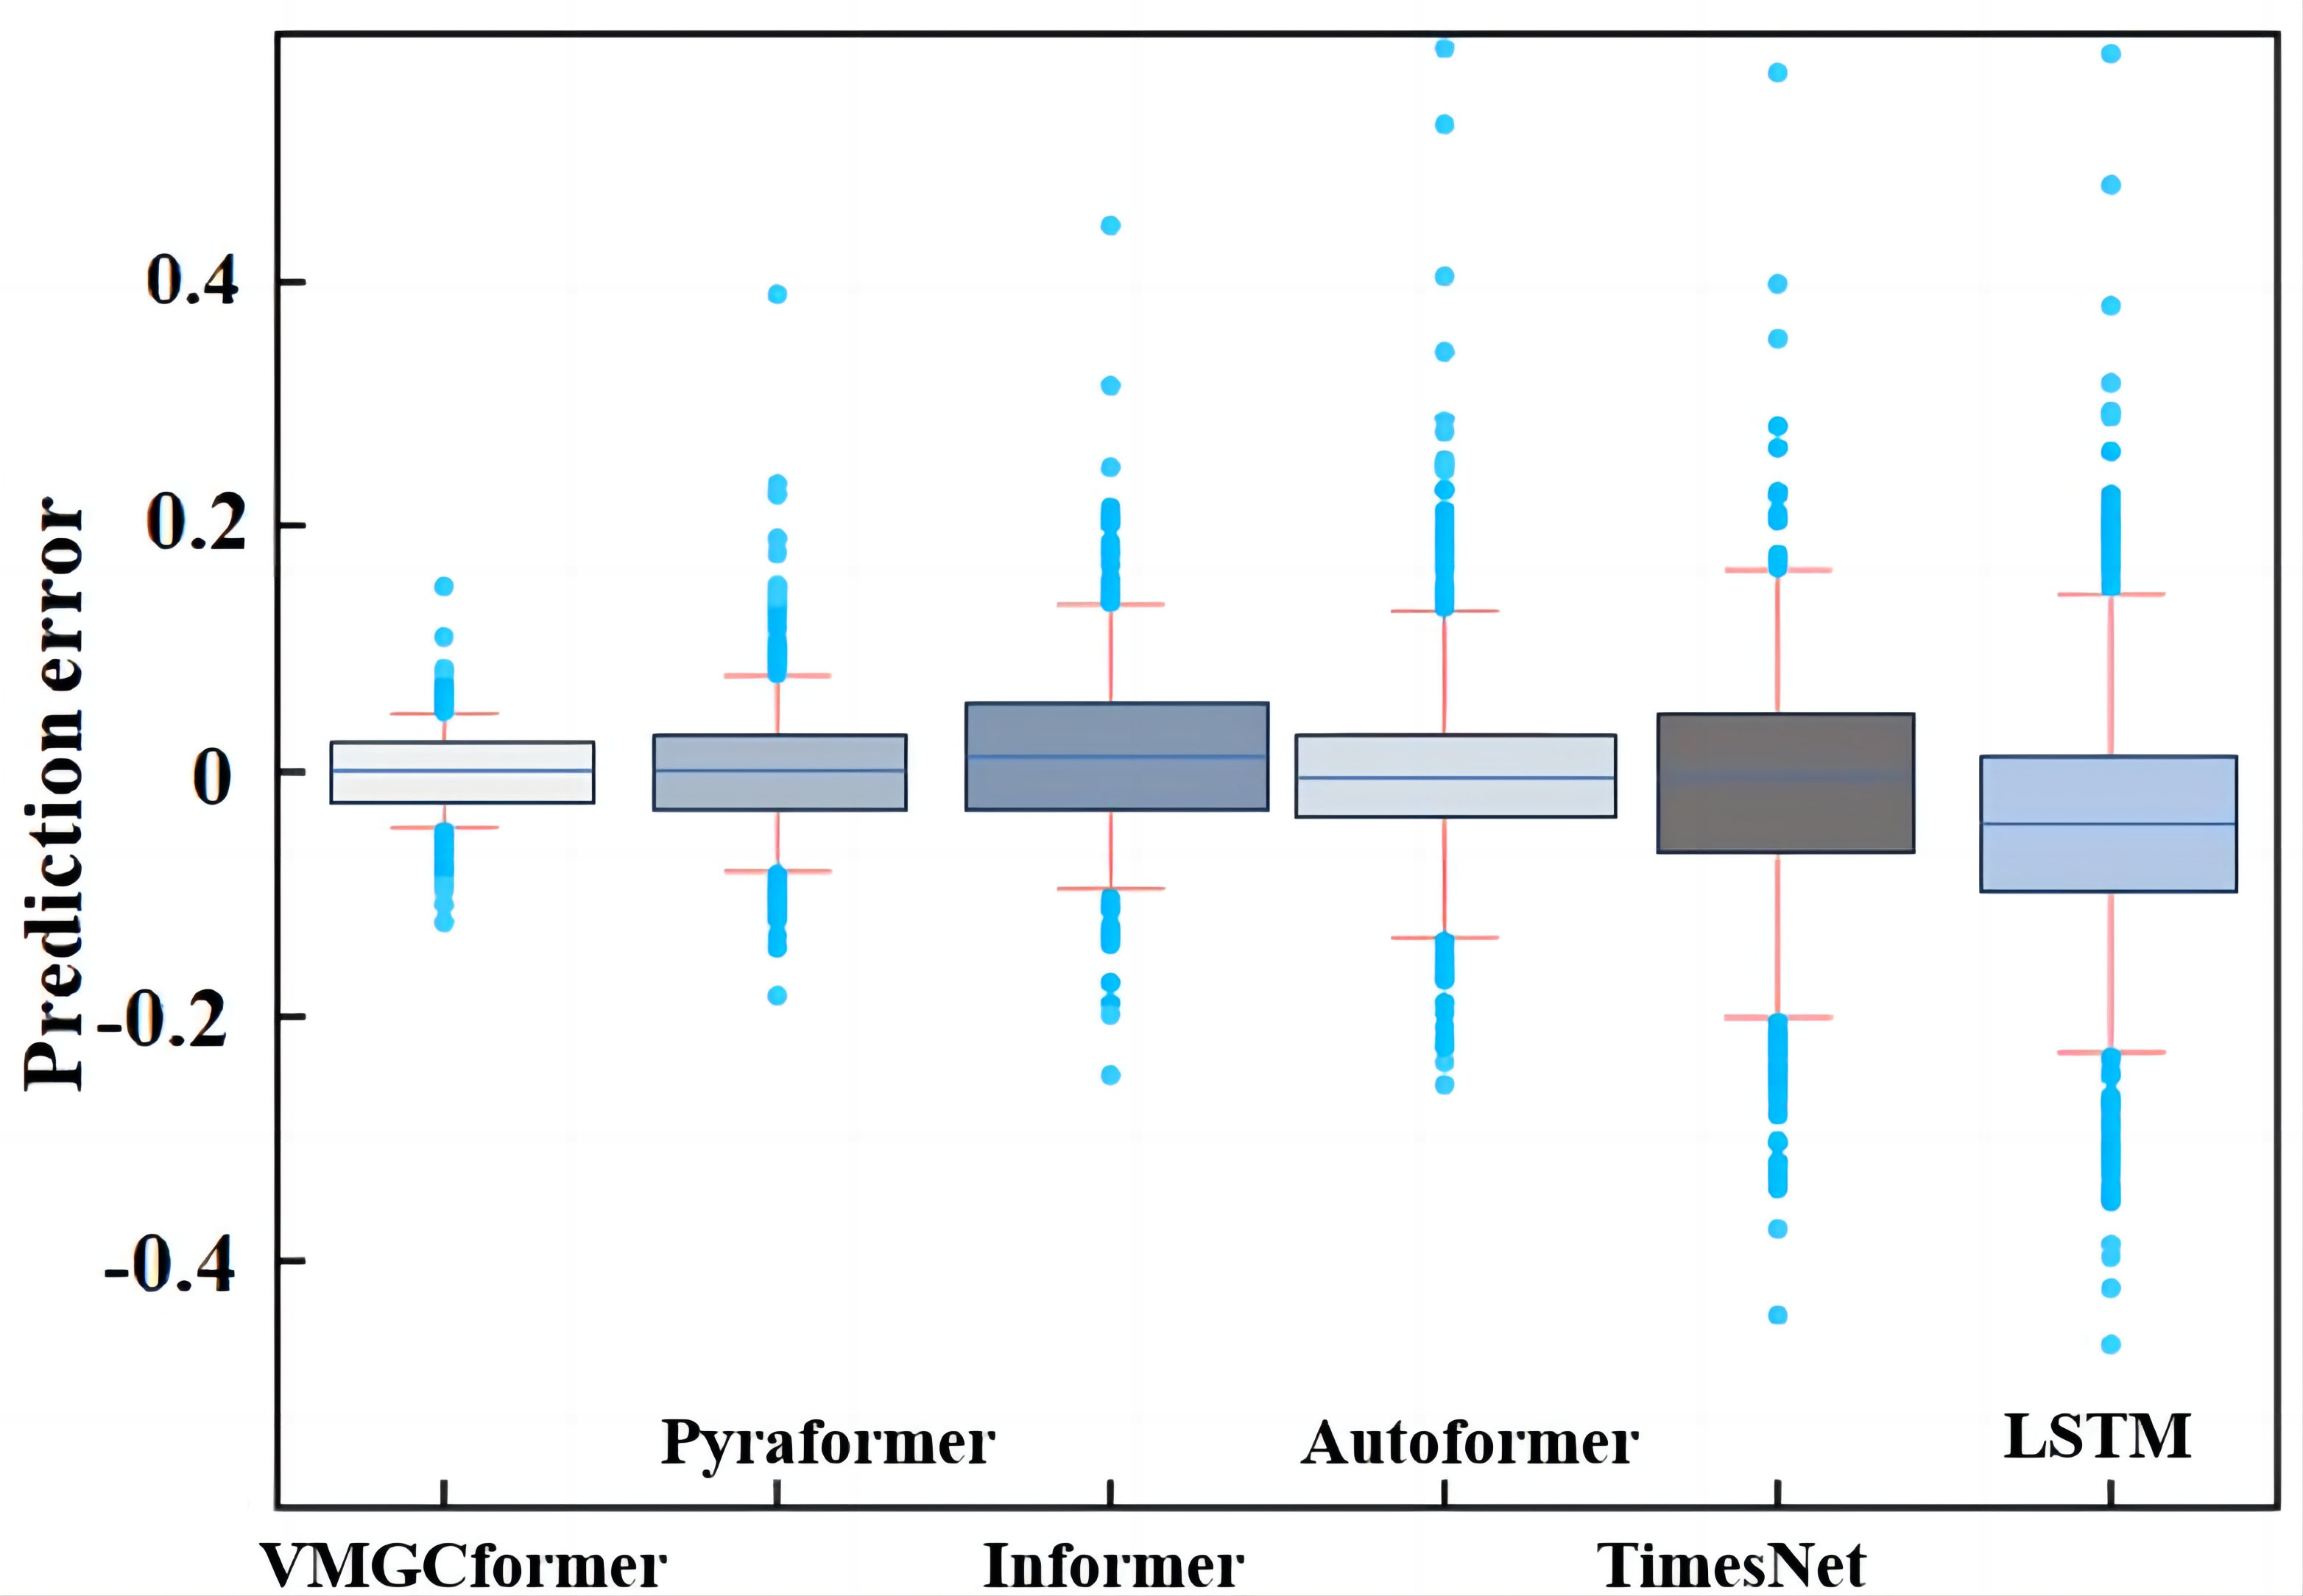
\includegraphics[width=0.7\textwidth]{pngs/case.png}
    \caption{ Box Plot of Prediction Errors For Some Models}
    \label{case}
\end{figure}

Based on the data presented in the charts and the analyzed characteristics, we can derive the following insights:

\begin{enumerate}
\item \textbf{Outstanding Performance}: 
The VMGCformer model consistently excels across all evaluation metrics, surpassing both individual predictive models and other composite models. Specifically, the MAE has been reduced by at least 45.45\% compared to other models, the RMSE by at least 40.04\%, and the \(R^2\) has seen an approximate increase of 7.09\%.
    
\item \textbf{Decomposition Prowess}: 
Analyzing curve characteristics reveals that, under similar data processing conditions, the IVMD algorithm demonstrates superior data decomposition capabilities compared to the traditional EMD algorithm. This enhances the stock prediction accuracy by effectively attenuating non-smooth features in the original data.
    
\item \textbf{Comparative Superiority}:
Under the same data processing methods, VMGCformer significantly outperforms both the Informer and LSTM, with \(R^2\) values of 0.925, 0.889, and 0.808 respectively.
    
\item \textbf{Time Efficiency Considerations}: While the prediction speed of VMGCformer is comparable to other models, the time overhead slightly increases due to the execution of ten Ad-Informer prediction modules post the IVMD-FE data preprocessing.
    
\item \textbf{Long-Term Forecasting Capability}:
Further data analysis indicates a trend wherein, during extended forecasting, the curve fit of different models begins to diverge. While most curves maintain a high degree of fit initially, they start deviating from the actual values over time. However, the VMGCformer maintains its prediction accuracy, highlighting its proficiency in addressing the challenges of long-time series forecasting.
\end{enumerate}

In conclusion, VMGCformer represents a superior predictive combination model, holding significant practical implications, especially in domains like long-term investment decisions, risk management, and asset allocation.


\subsubsection{Stability Experiment}\label{subsubsec3}
Previous experimental results indicate that VMGCformer outperforms other benchmark models on the China Petroleum stock dataset, demonstrating considerable capabilities in long-time series forecasting. However, stock prices, as intricate financial time series indices, can exhibit unpredictability due to variations in their industrial sectors, unforeseen events, shifts in market sentiment, and the interplay of chaotic factors. To further scrutinize the model's stability and applicability, we expanded our study to include four stocks from diverse sectors, each with distinct price trends and variances. These stocks are: ZTE Corporation (sz.000063), China Petroleum \& Chemical Corporation (sh.600028), Shanghai Pudong Development Bank (sh.600000), and Dongfeng Motor Corporation (sh.600006).

Under the premise of retaining the original parameter settings, the results of the predictions for the four stocks using VMGCformer are illustrated in Fig. \ref{stable}. The corresponding error values can be found in Table \ref{error_stable}

\begin{figure}[h]
    \centering
    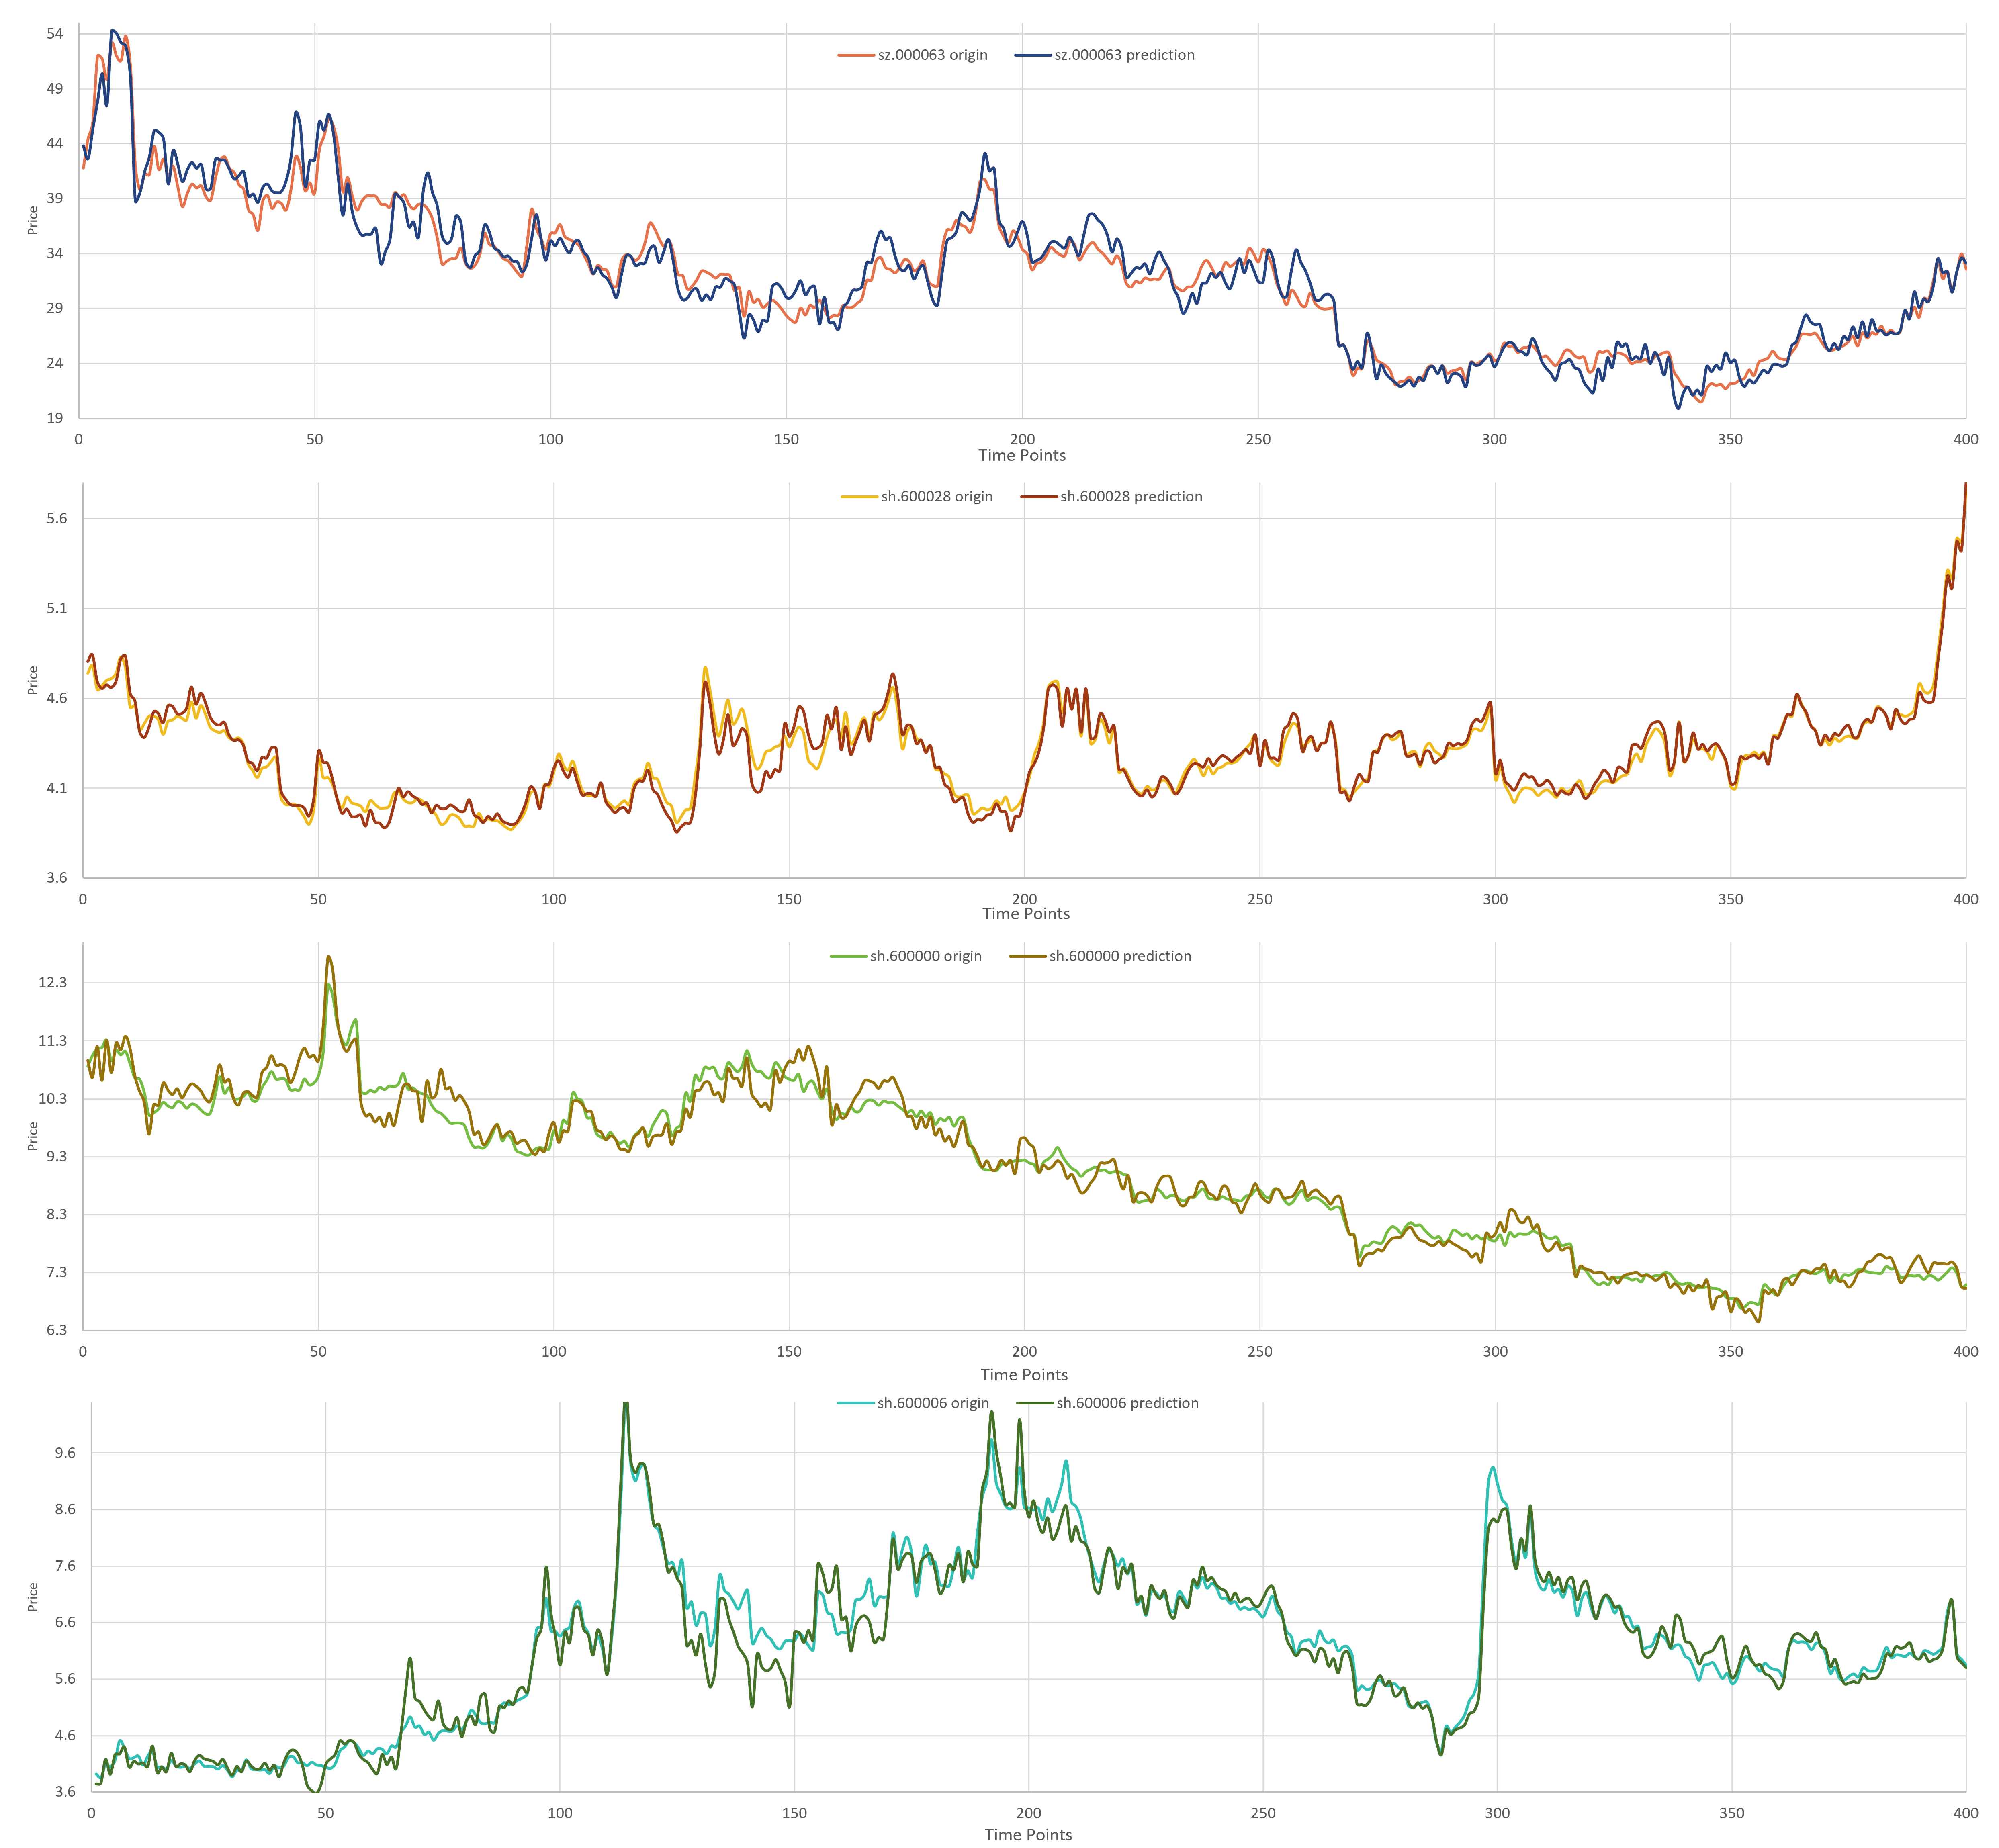
\includegraphics[width=1\textwidth]{pngs/stable.png}
    \caption{ Results For Stability Experiment}
    \label{stable}
\end{figure}

\begin{table}[h]
\caption{Forecasting Errors for Selected Stocks using VMGCformer}\label{error_stable}
\centering
\begin{tabular}{@{}lccc@{}}
\toprule
\textbf{Stock} & \textbf{MAE} & \textbf{RMSE} & \textbf{\(R^2\)} \\
\midrule
sz.000063 & 1.24991 & 1.64381 & 0.961253 \\
sh.600028 & 0.0399661 & 0.0509714 & 0.958723 \\
sh.600000 & 1.15268 & 1.48779 & 0.947264 \\
sh.600006 & 0.181266 & 0.231195 & 0.970125 \\
\bottomrule
\end{tabular}
\end{table}

Based on the analysis of charted results, stocks from four major corporations spanning the chemical, technology, transportation, and financial sectors have demonstrated commendable accuracy under the predictions of the VMGCformer model. However, it is noteworthy that for stocks sz.000063 and sh.600000, the MAE and RMSE values are significantly elevated. This disparity can largely be attributed to the considerably higher stock prices of these two entities compared to the others. Nonetheless, it is reasonable to conclude that the VMGCformer model, as proposed in this study, exhibits high stability and generalization capabilities across diverse datasets.


\section{Conclusions \& future work}\label{sec5}
\subsection{Conclusions}\label{sec5.1}
The operation of stock markets is influenced by various factors, such as economic conditions, seasonal fluctuations, and the global financial environment. These elements can introduce numerous anomalies and non-smooth characteristics into stock market data, posing significant challenges to enhancing the accuracy and performance of stock price predictions. Hence, this paper introduces an adaptive hybrid model for stock predictions, based on an improved VMD, FE, stacked Informer, and adaptive loss function. The Adam+GC+enhanced informer model emerges as a promising hybrid model capable of adaptively predicting stock data with inherent volatility. The main advantages of this approach are summarized as follows:

\begin{itemize}
    \item \textbf{Hybrid Integration}: The Adam+GC+enhanced informer serves as an integrated model, amalgamating the strengths of various techniques to offer superior accuracy and robustness compared to foundational models like CNN, LSTM, and other hybrid counterparts. This superiority is notably retained in long-time series forecasting.
    
    \item \textbf{Data Decomposition}: The MIC-enhanced VMD excels in extracting non-linear features from raw data compared to conventional decomposition methods, effectively enhancing data quality and simplifying the prediction process.
    
    \item \textbf{Adaptive Response}: Comprehensive analysis of experimental results showcases the rapid responsiveness of the adaptive loss function to volatile financial time series data, adeptly handling anomalies and predicting evolving trends.
    
    \item \textbf{Generalization Capability}: Experiments conducted on additional stock datasets underscore the exemplary predictive outcomes of our proposed model, affirming the significant generalization capabilities and promising prospects of the Adam+GC+enhanced informer in stock data forecasting.
\end{itemize}

In summary, hybrid stock prediction models, which amalgamate the advantages of multiple algorithms, demonstrate heightened prediction accuracy and robustness. Particularly, their efficacy remains undiminished in long-time series forecasting.


\subsection{Future Work}\label{sec5.2}

While this study has made preliminary advancements, various aspects warrant further exploration to enrich our understanding and practical application of stock market prediction models. Below are potential research directions:

\begin{itemize}
    \item \textbf{Predictive Modeling for Small Enterprises}: One limitation of our study is the primary focus on large-scale enterprise stocks. However, stock prices of smaller firms may be more sensitive and vulnerable to unforeseen events. Future research could emphasize integrating natural language processing and real-time event analysis to more precisely predict stock fluctuations of smaller firms. Given the non-linear impact of such sudden events on stock prices, it would be judicious to introduce specific parameters or variables to aptly capture these effects.
    
    \item \textbf{Non-linear Optimization in Feature Engineering}: Another shortcoming in our study pertains to the predominantly linear approach employed in our feature engineering design. Subsequent studies might consider non-linear methods, such as activation functions in neural networks or dynamically learned weight coefficients. This approach can perpetually optimize feature value generation during iterative learning, bolstering model performance and adaptability.
    
    \item \textbf{Further Optimizations and Refinements}: We've identified two potential avenues for enhancement. Firstly, our feature selection only considered correlation factors, neglecting metrics like F-score and sensitivity. Future endeavors will attempt to utilize F-score and sensitivity to analyze relationships between other variables and stock characteristics, aiming to curtail data redundancy. Secondly, the parameter selection in our study may lack precision and comprehensiveness. To address this, we'll contemplate the integration of optimization algorithms to mitigate sensitivity issues inherent in deep learning network parameter selection.
\end{itemize}

With a deeper dive into the aforementioned research directions, we anticipate further improvements in the precision, utility, and comprehensiveness of stock market prediction models. This advancement will not only propel academic research in the financial domain but also furnish practitioners with more accurate decision-support tools, aiding in navigating the multifaceted challenges of financial markets.



\begin{thebibliography}{100}

\bibitem[{Tsay(2005)}]{tsay2005analysis}
\bibinfo{author}{Ruey S. Tsay},
\bibinfo{year}{2005}.
\newblock \bibinfo{title}{Analysis of financial time series}.
\newblock \bibinfo{publisher}{John Wiley \& Sons}.



\bibitem[{Mandelbrot and Hudson(2010)}]{mandelbrot2010mis}
\bibinfo{author}{Benoit B. Mandelbrot}, \bibinfo{author}{Richard L. Hudson},
\bibinfo{year}{2010}.
\newblock \bibinfo{title}{The (mis) behaviour of markets: a fractal view of risk, ruin and reward}.
\newblock \bibinfo{publisher}{Profile books}.



\bibitem[{Brockwell and Davis(2002)}]{brockwell2002introduction}
\bibinfo{author}{Peter J. Brockwell}, \bibinfo{author}{Richard A. Davis},
\bibinfo{year}{2002}.
\newblock \bibinfo{title}{Introduction to time series and forecasting}.
\newblock \bibinfo{publisher}{Springer}.



\bibitem[{Huang et al.(1998)}]{huang1998empirical}
\bibinfo{author}{Norden E Huang}, \bibinfo{author}{Zheng Shen}, \bibinfo{author}{Steven R Long}, \bibinfo{author}{Manli C Wu}, \bibinfo{author}{Hsing H Shih}, \bibinfo{author}{Quanan Zheng}, \bibinfo{author}{Nai-Chyuan Yen}, \bibinfo{author}{Chi Chao Tung}, \bibinfo{author}{Henry H Liu},
\bibinfo{year}{1998}.
\newblock \bibinfo{title}{The empirical mode decomposition and the Hilbert spectrum for nonlinear and non-stationary time series analysis}.
\newblock \bibinfo{journal}{Proceedings of the Royal Society of London. Series A: mathematical, physical and engineering sciences} \bibinfo{volume}{454}(1971), \bibinfo{pages}{903--995}. \bibinfo{publisher}{The Royal Society}.



\bibitem[{Huang and Jiang(2022)}]{huang2022wind}
\bibinfo{author}{Xiaohan Huang}, \bibinfo{author}{Aihua Jiang},
\bibinfo{year}{2022}.
\newblock \bibinfo{title}{Wind Power Generation Forecast Based on Multi-Step Informer Network}.
\newblock \bibinfo{journal}{Energies} \bibinfo{volume}{15}(18), \bibinfo{pages}{6642}. \bibinfo{publisher}{MDPI}.



\bibitem[{Li et al.(2023)}]{li2023improving}
\bibinfo{author}{Feiyu Li}, \bibinfo{author}{Zhibo Wan}, \bibinfo{author}{Thomas Koch}, \bibinfo{author}{Guokuan Zan}, \bibinfo{author}{Mengjiao Li}, \bibinfo{author}{Zhonghai Zheng}, \bibinfo{author}{Bo Liang},
\bibinfo{year}{2023}.
\newblock \bibinfo{title}{Improving the accuracy of multi-step prediction of building energy consumption based on EEMD-PSO-Informer and long-time series}.
\newblock \bibinfo{journal}{Computers and Electrical Engineering} \bibinfo{volume}{110}, \bibinfo{pages}{108845}. \bibinfo{publisher}{Elsevier}.



\bibitem[{Gong et al.(2022)}]{gong2022load}
\bibinfo{author}{Mingju Gong}, \bibinfo{author}{Yin Zhao}, \bibinfo{author}{Jiawang Sun}, \bibinfo{author}{Cuitian Han}, \bibinfo{author}{Guannan Sun}, \bibinfo{author}{Bo Yan},
\bibinfo{year}{2022}.
\newblock \bibinfo{title}{Load forecasting of district heating system based on Informer}.
\newblock \bibinfo{journal}{Energy} \bibinfo{volume}{253}, \bibinfo{pages}{124179}. \bibinfo{publisher}{Elsevier}.


\bibitem[{Lee et al.(2023)}]{lee2023financial}
\bibinfo{author}{John Lee}, \bibinfo{author}{Jow-Ran Chang}, \bibinfo{author}{Lie-Jane Kao}, \bibinfo{author}{Cheng-Few Lee},
\bibinfo{year}{2023}.
\newblock \bibinfo{title}{Financial Analysis, Planning, and Forecasting}.
\newblock In: \bibinfo{booktitle}{Essentials of Excel VBA, Python, and R: Volume II: Financial Derivatives, Risk Management and Machine Learning}, \bibinfo{pages}{433--455}. \bibinfo{publisher}{Springer}.



\bibitem[{Jerez and Kristjanpoller(2020)}]{jerez2020effects}
\bibinfo{author}{Tomas Jerez}, \bibinfo{author}{Werner Kristjanpoller},
\bibinfo{year}{2020}.
\newblock \bibinfo{title}{Effects of the validation set on stock returns forecasting}.
\newblock \bibinfo{journal}{Expert Systems with Applications} \bibinfo{volume}{150}, \bibinfo{pages}{113271}. \bibinfo{publisher}{Elsevier}.



\bibitem[{Zhang et al.(2018)}]{zhang2018stock}
\bibinfo{author}{Xi Zhang}, \bibinfo{author}{Siyu Qu}, \bibinfo{author}{Jieyun Huang}, \bibinfo{author}{Binxing Fang}, \bibinfo{author}{Philip Yu},
\bibinfo{year}{2018}.
\newblock \bibinfo{title}{Stock market prediction via multi-source multiple instance learning}.
\newblock \bibinfo{journal}{IEEE Access} \bibinfo{volume}{6}, \bibinfo{pages}{50720--50728}. \bibinfo{publisher}{IEEE}.



\bibitem[{Kurani et al.(2023)}]{kurani2023comprehensive}
\bibinfo{author}{Akshit Kurani}, \bibinfo{author}{Pavan Doshi}, \bibinfo{author}{Aarya Vakharia}, \bibinfo{author}{Manan Shah},
\bibinfo{year}{2023}.
\newblock \bibinfo{title}{A comprehensive comparative study of artificial neural network (ANN) and support vector machines (SVM) on stock forecasting}.
\newblock \bibinfo{journal}{Annals of Data Science} \bibinfo{volume}{10}(\bibinfo{number}{1}), \bibinfo{pages}{183--208}. \bibinfo{publisher}{Springer}.



\bibitem[Sezer and Ozbayoglu(2018)]{sezer2018algorithmic}
Omer Berat Sezer, Ahmet Murat Ozbayoglu,
\newblock "Algorithmic financial trading with deep convolutional neural networks: Time series to image conversion approach",
\newblock {Applied Soft Computing}, 70, 525--538, 2018. Elsevier.



\bibitem[{Zaremba and Demir(2023)}]{zaremba2023chatgpt}
\bibinfo{author}{Adam Zaremba}, \bibinfo{author}{Ender Demir},
\bibinfo{year}{2023}.
\newblock \bibinfo{title}{ChatGPT: Unlocking the future of NLP in finance}.
\newblock \bibinfo{journal}{Available at SSRN 4323643}.


\bibitem[{Engle(1982)}]{engle1982autoregressive}
\bibinfo{author}{Robert F. Engle},
\bibinfo{year}{1982}.
\newblock \bibinfo{title}{Autoregressive conditional heteroscedasticity with estimates of the variance of United Kingdom inflation}.
\newblock \bibinfo{journal}{Econometrica: Journal of the econometric society} \bibinfo{volume}{}, \bibinfo{pages}{987--1007}. \bibinfo{publisher}{JSTOR}.


\bibitem[{Bollerslev(1986)}]{bollerslev1986generalized}
\bibinfo{author}{Tim Bollerslev},
\bibinfo{year}{1986}.
\newblock \bibinfo{title}{Generalized autoregressive conditional heteroskedasticity}.
\newblock \bibinfo{journal}{Journal of econometrics} \bibinfo{volume}{31}(\bibinfo{number}{3}), \bibinfo{pages}{307--327}. \bibinfo{publisher}{Elsevier}.



\bibitem[{Hsieh(1988)}]{hsieh1988statistical}
\bibinfo{author}{David A. Hsieh},
\bibinfo{year}{1988}.
\newblock \bibinfo{title}{The statistical properties of daily foreign exchange rates: 1974--1983}.
\newblock \bibinfo{journal}{Journal of international economics} \bibinfo{volume}{24}(1-2), \bibinfo{pages}{129--145}. \bibinfo{publisher}{Elsevier}.



\bibitem[{Brown(2004)}]{brown2004smoothing}
\bibinfo{author}{Robert Goodell Brown},
\bibinfo{year}{2004}.
\newblock \bibinfo{title}{Smoothing, forecasting and prediction of discrete time series}.
\newblock \bibinfo{publisher}{Courier Corporation}.


\bibitem[{Wang et al.(2022)}]{wang2022asian}
\bibinfo{author}{Wang, Jujie}, \bibinfo{author}{Cui, Quan}, \bibinfo{author}{Sun, Xin}, \bibinfo{author}{He, Maolin},
\bibinfo{year}{2022}.
\newblock \bibinfo{title}{Asian stock markets closing index forecast based on secondary decomposition, multi-factor analysis and attention-based LSTM model}.
\newblock \bibinfo{journal}{Engineering Applications of Artificial Intelligence} \bibinfo{volume}{113}, \bibinfo{pages}{104908}. \bibinfo{publisher}{Elsevier}.


\bibitem[{Wang et al.(2020)}]{wang2020time}
\bibinfo{author}{Fang Wang, Menggang Li, Yiduo Mei, and Wenrui Li},
\bibinfo{year}{2020}.
\newblock \bibinfo{title}{Time series data mining: A case study with big data analytics approach}.
\newblock \bibinfo{journal}{IEEE Access} \bibinfo{volume}{8}, \bibinfo{pages}{14322--14328}. \bibinfo{publisher}{IEEE}.


\bibitem[{Herwartz(2017)}]{herwartz2017stock}
\bibinfo{author}{Helmut Herwartz},
\bibinfo{year}{2017}.
\newblock \bibinfo{title}{Stock return prediction under GARCH—An empirical assessment}.
\newblock \bibinfo{journal}{International Journal of Forecasting} \bibinfo{volume}{33}(\bibinfo{number}{3}), \bibinfo{pages}{569--580}. \bibinfo{publisher}{Elsevier}.


\bibitem[{Pomponi et al.(2021)}]{pomponi2021structured}
\bibinfo{author}{Jary Pomponi}, \bibinfo{author}{Simone Scardapane}, \bibinfo{author}{Aurelio Uncini},
\bibinfo{year}{2021}.
\newblock \bibinfo{title}{Structured Ensembles: An approach to reduce the memory footprint of ensemble methods}.
\newblock \bibinfo{journal}{Neural Networks} \bibinfo{volume}{144}, \bibinfo{pages}{407--418}. \bibinfo{publisher}{Elsevier}.

\bibitem[{Tung and Mori(2018)}]{tung2018clip}
\bibinfo{author}{Frederick Tung}, \bibinfo{author}{Greg Mori},
\bibinfo{year}{2018}.
\newblock \bibinfo{title}{Clip-q: Deep network compression learning by in-parallel pruning-quantization}.
\newblock \bibinfo{journal}{Proceedings of the IEEE conference on computer vision and pattern recognition} \bibinfo{pages}{7873--7882}.

\bibitem[{Yang and Lin(2016)}]{yang2016integrated}
\bibinfo{author}{Heng-Li Yang}, \bibinfo{author}{Han-Chou Lin},
\bibinfo{year}{2016}.
\newblock \bibinfo{title}{An integrated model combined ARIMA, EMD with SVR for stock indices forecasting}.
\newblock \bibinfo{journal}{International Journal on Artificial Intelligence Tools} \bibinfo{volume}{25}, \bibinfo{pages}{1650005}. \bibinfo{publisher}{World Scientific}.

\bibitem[{Alfonso et al.(2020)}]{alfonso2020stock}
\bibinfo{author}{Gerardo Alfonso}, \bibinfo{author}{A Daniel Carnerero}, \bibinfo{author}{Daniel R Ramirez}, \bibinfo{author}{Teodoro Alamo},
\bibinfo{year}{2020}.
\newblock \bibinfo{title}{Stock forecasting using local data}.
\newblock \bibinfo{journal}{IEEE Access} \bibinfo{volume}{9}, \bibinfo{pages}{9334--9344}. \bibinfo{publisher}{IEEE}.

\bibitem[{Bukhari et al.(2020)}]{bukhari2020fractional}
\bibinfo{author}{Ayaz Hussain Bukhari}, \bibinfo{author}{Muhammad Asif Zahoor Raja}, \bibinfo{author}{Muhammad Sulaiman}, \bibinfo{author}{Saeed Islam}, \bibinfo{author}{Muhammad Shoaib}, \bibinfo{author}{Poom Kumam},
\bibinfo{year}{2020}.
\newblock \bibinfo{title}{Fractional neuro-sequential ARFIMA-LSTM for financial market forecasting}.
\newblock \bibinfo{journal}{IEEE Access} \bibinfo{volume}{8}, \bibinfo{pages}{71326--71338}. \bibinfo{publisher}{IEEE}.

\bibitem[{Büyükşahin and Ertekin(2019)}]{buyukcsahin2019improving}
\bibinfo{author}{Ümit Çavuş Büyükşahin}, \bibinfo{author}{Şeyda Ertekin},
\bibinfo{year}{2019}.
\newblock \bibinfo{title}{Improving forecasting accuracy of time series data using a new ARIMA-ANN hybrid method and empirical mode decomposition}.
\newblock \bibinfo{journal}{Neurocomputing} \bibinfo{volume}{361}, \bibinfo{pages}{151--163}. \bibinfo{publisher}{Elsevier}.

\bibitem[{Qiu et al.(2020)}]{qiu2020novel}
\bibinfo{author}{Yue Qiu}, \bibinfo{author}{Hao-Yu Yang}, \bibinfo{author}{Shan Lu}, \bibinfo{author}{Wei Chen},
\bibinfo{year}{2020}.
\newblock \bibinfo{title}{A novel hybrid model based on recurrent neural networks for stock market timing}.
\newblock \bibinfo{journal}{Soft Computing} \bibinfo{volume}{24}, \bibinfo{pages}{15273--15290}. \bibinfo{publisher}{Springer}.

\bibitem[{Jin et al.(2020)}]{jin2020stock}
\bibinfo{author}{Zhigang Jin}, \bibinfo{author}{Yang Yang}, \bibinfo{author}{Yuhong Liu},
\bibinfo{year}{2020}.
\newblock \bibinfo{title}{Stock closing price prediction based on sentiment analysis and LSTM}.
\newblock \bibinfo{journal}{Neural Computing and Applications} \bibinfo{volume}{32}, \bibinfo{pages}{9713--9729}. \bibinfo{publisher}{Springer}.




\bibitem[{Lu et al.(2021)}]{lu2021cnn}
\bibinfo{author}{Wenjie Lu}, \bibinfo{author}{Jiazheng Li}, \bibinfo{author}{Jingyang Wang}, \bibinfo{author}{Lele Qin},
\bibinfo{year}{2021}.
\newblock \bibinfo{title}{A CNN-BiLSTM-AM method for stock price prediction}.
\newblock \bibinfo{journal}{Neural Computing and Applications} \bibinfo{volume}{33}, \bibinfo{pages}{4741--4753}. \bibinfo{publisher}{Springer}.

\bibitem[{Chen et al.(2022)}]{chen2022china}
\bibinfo{author}{Yufeng Chen}, \bibinfo{author}{Jinwang Wu}, \bibinfo{author}{Zhongrui Wu},
\bibinfo{year}{2022}.
\newblock \bibinfo{title}{China’s commercial bank stock price prediction using a novel K-means-LSTM hybrid approach}.
\newblock \bibinfo{journal}{Expert Systems with Applications} \bibinfo{volume}{202}, \bibinfo{pages}{117370}. \bibinfo{publisher}{Elsevier}.

\bibitem[{Guo et al.(2021)}]{guo2021mrc}
\bibinfo{author}{Qiutong Guo}, \bibinfo{author}{Shun Lei}, \bibinfo{author}{Qing Ye}, \bibinfo{author}{Zhiyang Fang},
\bibinfo{year}{2021}.
\newblock \bibinfo{title}{MRC-LSTM: a hybrid approach of multi-scale residual CNN and LSTM to predict bitcoin price}.
\newblock In \bibinfo{booktitle}{2021 International Joint Conference on Neural Networks (IJCNN)}, \bibinfo{pages}{1--8}. \bibinfo{organization}{IEEE}.

\bibitem[{Zhou et al.(2021)}]{zhou2021informer}
\bibinfo{author}{H. Zhou, S. Zhang, J. Peng, S. Zhang, J. Li, H. Xiong, W. Zhang},
\bibinfo{year}{2021}.
\newblock \bibinfo{title}{Informer: Beyond efficient transformer for long sequence time-series forecasting}.
\newblock \bibinfo{booktitle}{Proceedings of the AAAI conference on artificial intelligence}, \bibinfo{volume}{35}, \bibinfo{number}{12}, \bibinfo{pages}{11106--11115}.
\newblock \bibinfo{publisher}{AAAI Press}.



\bibitem[{Zhang et al.(2022)}]{zhang2022transformer}
\bibinfo{author}{Qiuyue Zhang}, \bibinfo{author}{Chao Qin}, \bibinfo{author}{Yunfeng Zhang}, \bibinfo{author}{Fangxun Bao}, \bibinfo{author}{Caiming Zhang}, \bibinfo{author}{Peide Liu},
\bibinfo{year}{2022}.
\newblock \bibinfo{title}{Transformer-based attention network for stock movement prediction}.
\newblock \bibinfo{journal}{Expert Systems with Applications} \bibinfo{volume}{202}, \bibinfo{pages}{117239}. \bibinfo{publisher}{Elsevier}.


\bibitem[Kim and Won(2018)]{kim2018forecasting}
Ha Young Kim, Chang Hyun Won,
\newblock "Forecasting the volatility of stock price index: A hybrid model integrating LSTM with multiple GARCH-type models",
\newblock {Expert Systems with Applications}, 103, 25--37, 2018. Elsevier.

\bibitem[Yang and Lin(2016)]{yang2016integrated}
Heng-Li Yang, Han-Chou Lin,
\newblock "An integrated model combined ARIMA, EMD with SVR for stock indices forecasting",
\newblock {International Journal on Artificial Intelligence Tools}, 25(02), 1650005, 2016. World Scientific.


\bibitem[Luo et al.(2021)]{luo2021hybrid}
Zhidan Luo, Wei Guo, Qingfu Liu, Zhengjun Zhang,
\newblock "A hybrid model for financial time-series forecasting based on mixed methodologies",
\newblock {Expert Systems}, 38(2), e12633, 2021. Wiley Online Library.



\bibitem[Du et al.(2019)]{du2019container}
Pei Du, Jianzhou Wang, Wendong Yang, Tong Niu,
\newblock "Container throughput forecasting using a novel hybrid learning method with error correction strategy",
\newblock {Knowledge-Based Systems}, 182, 104853, 2019. Elsevier.


\bibitem[Iftikhar et al.(2023)]{iftikhar2023forecasting}
Hasnain Iftikhar, Aimel Zafar, Josue E Turpo-Chaparro, Paulo Canas Rodrigues, Javier Linkolk López-Gonzales,
\newblock "Forecasting Day-Ahead Brent Crude Oil Prices Using Hybrid Combinations of Time Series Models",
\newblock {Mathematics}, 11(16), 3548, 2023. MDPI.


\bibitem[{Wei(2016)}]{wei2016hybrid}
\bibinfo{author}{Liang-Ying Wei},
\bibinfo{year}{2016}.
\newblock \bibinfo{title}{A hybrid ANFIS model based on empirical mode decomposition for stock time series forecasting}.
\newblock \bibinfo{journal}{Applied Soft Computing}, \bibinfo{volume}{42}, \bibinfo{pages}{368--376}. \bibinfo{publisher}{Elsevier}.

\bibitem[{Rubio and Alba(2022)}]{rubio2022forecasting}
\bibinfo{author}{Lihki Rubio}, \bibinfo{author}{Keyla Alba},
\bibinfo{year}{2022}.
\newblock \bibinfo{title}{Forecasting selected colombian shares using a hybrid ARIMA-SVR model}.
\newblock \bibinfo{journal}{Mathematics}, \bibinfo{volume}{10}(13), \bibinfo{pages}{2181}. \bibinfo{publisher}{MDPI}.

\bibitem[{Li et al.(2020)}]{li2020fractional}
\bibinfo{author}{Shuqi Li}, \bibinfo{author}{Xiaoming Liu}, \bibinfo{author}{Aijing Lin},
\bibinfo{year}{2020}.
\newblock \bibinfo{title}{Fractional frequency hybrid model based on EEMD for financial time series forecasting}.
\newblock \bibinfo{journal}{Communications in Nonlinear Science and Numerical Simulation}, \bibinfo{volume}{89}, \bibinfo{pages}{105281}. \bibinfo{publisher}{Elsevier}.

\bibitem[{Singh et al.(2021)}]{singh2021soft}
\bibinfo{author}{Sarbjit Singh}, \bibinfo{author}{Kulwinder Singh Parmar}, \bibinfo{author}{Jatinder Kumar},
\bibinfo{year}{2021}.
\newblock \bibinfo{title}{Soft computing model coupled with statistical models to estimate future of stock market}.
\newblock \bibinfo{journal}{Neural Computing and Applications}, \bibinfo{volume}{33}, \bibinfo{pages}{7629--7647}. \bibinfo{publisher}{Springer}.




%%%%%%%%%%%%%%%%%%%%%%%%%%%%%%%%%%%%%%%%%%%%





\bibitem[{Kara et al.(2011)}]{kara2011prediction}
\bibinfo{author}{Yakup Kara}, \bibinfo{author}{Melek Acar Boyacioglu}, \bibinfo{author}{Ömer Kaan Baykan},
\bibinfo{year}{2011}.
\newblock \bibinfo{title}{Predicting direction of stock price index movement using artificial neural networks and support vector machines: The sample of the Istanbul Stock Exchange}.
\newblock \bibinfo{journal}{Expert systems with Applications} \bibinfo{volume}{38}(5), \bibinfo{pages}{5311--5319}. \bibinfo{publisher}{Elsevier}.

\bibitem[{Guresen et al.(2011)}]{guresen2011using}
\bibinfo{author}{Erkam Guresen}, \bibinfo{author}{Gulgun Kayakutlu}, \bibinfo{author}{Tugrul U Daim},
\bibinfo{year}{2011}.
\newblock \bibinfo{title}{Using artificial neural network models in stock market index prediction}.
\newblock \bibinfo{journal}{Expert systems with Applications} \bibinfo{volume}{38}(8), \bibinfo{pages}{10389--10397}. \bibinfo{publisher}{Elsevier}.



\bibitem[{Achelis(2005)}]{achelis2005technical}
\bibinfo{author}{S.B. Achelis},
\bibinfo{year}{2005}.
\newblock \bibinfo{title}{Technical Analysis From A To Z}.
\newblock \bibinfo{publisher}{Vision Books}. \bibinfo{url}{https://books.google.com/books?id=J1YDPgAACAAJ}



\bibitem[{Dragomiretskiy and Zosso(2013)}]{dragomiretskiy2013variational}
\bibinfo{author}{K. Dragomiretskiy, D. Zosso},
\bibinfo{year}{2013}.
\newblock \bibinfo{title}{Variational mode decomposition}.
\newblock \bibinfo{journal}{IEEE transactions on signal processing}, \bibinfo{volume}{62}(\bibinfo{number}{3}), \bibinfo{pages}{531--544}.
\newblock \bibinfo{publisher}{IEEE}.


\bibitem[{Lin et al.(2022)}]{lin2022using}
\bibinfo{author}{G. Lin, A. Lin, D. Gu},
\bibinfo{year}{2022}.
\newblock \bibinfo{title}{Using support vector regression and K-nearest neighbors for short-term traffic flow prediction based on maximal information coefficient}.
\newblock \bibinfo{journal}{Information Sciences}, \bibinfo{volume}{608}, \bibinfo{pages}{517--531}.
\newblock \bibinfo{publisher}{Elsevier}.


\bibitem[{Chen et al.(2009)}]{chen2009measuring}
\bibinfo{author}{W. Chen, J. Zhuang, W. Yu, Z. Wang},
\bibinfo{year}{2009}.
\newblock \bibinfo{title}{Measuring complexity using fuzzyen, apen, and sampen}.
\newblock \bibinfo{journal}{Medical Engineering \& Physics}, \bibinfo{volume}{31}, \bibinfo{number}{1}, \bibinfo{pages}{61--68}.
\newblock \bibinfo{publisher}{Elsevier}.


\bibitem[{Vaswani et al.(2017)}]{vaswani2017attention}
\bibinfo{author}{A. Vaswani, N. Shazeer, N. Parmar, J. Uszkoreit, L. Jones, A.N. Gomez, {\L}. Kaiser, I. Polosukhin},
\bibinfo{year}{2017}.
\newblock \bibinfo{title}{Attention is all you need}.
\newblock \bibinfo{journal}{Advances in neural information processing systems}, \bibinfo{volume}{30}.
\newblock \bibinfo{publisher}{NIPS}.

\bibitem[{Selvin et al.(2017)}]{selvin2017stock}
\bibinfo{author}{S. Selvin, R. Vinayakumar, E.A. Gopalakrishnan, V.K. Menon, K.P. Soman},
\bibinfo{year}{2017}.
\newblock \bibinfo{title}{Stock price prediction using LSTM, RNN and CNN-sliding window model}.
\newblock \bibinfo{booktitle}{2017 international conference on advances in computing, communications and informatics (icacci)}, \bibinfo{pages}{1643--1647}.
\newblock \bibinfo{publisher}{IEEE}.

\bibitem[{Ye et al.(2019)}]{ye2019river}
\bibinfo{author}{Q. Ye, X. Yang, C. Chen, J. Wang},
\bibinfo{year}{2019}.
\newblock \bibinfo{title}{River water quality parameters prediction method based on LSTM-RNN model}.
\newblock \bibinfo{booktitle}{2019 Chinese Control And Decision Conference (CCDC)}, \bibinfo{pages}{3024--3028}.
\newblock \bibinfo{publisher}{IEEE}.


\bibitem[{Pascanu et al.(2013)}]{pascanu2013difficulty}
\bibinfo{author}{R. Pascanu, T. Mikolov, Y. Bengio},
\bibinfo{year}{2013}.
\newblock \bibinfo{title}{On the difficulty of training recurrent neural networks}.
\newblock \bibinfo{booktitle}{International conference on machine learning}, \bibinfo{pages}{1310--1318}.
\newblock \bibinfo{publisher}{Pmlr}.


\bibitem[{Barron(2019)}]{barron2019general}
\bibinfo{author}{J. T. Barron},
\bibinfo{year}{2019}.
\newblock \bibinfo{title}{A general and adaptive robust loss function}.
\newblock \bibinfo{booktitle}{Proceedings of the IEEE/CVF Conference on Computer Vision and Pattern Recognition}, \bibinfo{pages}{4331--4339}.
\newblock \bibinfo{publisher}{IEEE/CVF}.

\bibitem[{Yong et al.(2020)}]{yong2020gradient}
\bibinfo{author}{Hongwei Yong}, \bibinfo{author}{Jianqiang Huang}, \bibinfo{author}{Xiansheng Hua}, \bibinfo{author}{Lei Zhang},
\bibinfo{year}{2020}.
\newblock \bibinfo{title}{Gradient centralization: A new optimization technique for deep neural networks}.
\newblock \bibinfo{journal}{Computer Vision--ECCV 2020: 16th European Conference, Glasgow, UK, August 23--28, 2020, Proceedings, Part I 16} \bibinfo{volume}{}, \bibinfo{pages}{635--652}. \bibinfo{publisher}{Springer}.




 
\end{thebibliography}
\end{document}
